\documentclass[twoside,11pt]{article}
\usepackage{jmlr2e}            % <- uncomment for JMLR submission
%\usepackage{jmlr2e-stripped}    % <- uncomment for arXiv version

\usepackage{amsmath,amsfonts}
\usepackage{url}
\usepackage[usenames,dvipsnames,svgnames,table]{xcolor}

\usepackage{algorithm}
\usepackage{algpseudocode}
\usepackage{caption}
\usepackage{comment}
\usepackage{dsfont}
\usepackage{graphicx,verbatim}
\usepackage{listings}
\usepackage{subcaption}
\usepackage{todonotes}

\usepackage{tikz}
\usetikzlibrary{arrows}

\frenchspacing
\hyphenation{speed-up}
\hyphenation{ProPublica}

\newcommand{\eanote}[1]{{\color{magenta} (EA) #1}}
\newcommand{\red}[1]{{\color{red} #1}}
\newcommand{\yellow}[1]{{\color{yellow} #1}}
\newcommand{\green}[1]{{\color{green} #1}}
\newcommand{\eat}[1]{ }

\def\ie{{\it i.e.},~}
\def\eg{{\it e.g.},~}
\def\etal{{\it et al.}~}
\def\bif{\bf if~}
\def\belif{{\bf else if~}}
\def\bthen{{\bf then predict~}}
\def\belse{{\bf else predict~}}

\def\E{\mathbb{E}}
\def\P{\mathbb{P}}
\def\Var{\mbox{Var}}
\def\Unif{\mbox{Unif}}
\def\Normal{\mbox{Normal}}
\def\reals{\mathbb{R}}
\def\ints{\mathbb{Z}}
\def\one{\mathds{1}}
\def\Normal{\mathrm{Normal}}
\def\X{{\mathcal X}}
\def\Y{{\mathcal Y}}
\def\N{{\mathcal N}}

\newcommand{\x}{\mathbf{x}}
\newcommand{\y}{\mathbf{y}}
\def\RL{{d}}
\def\Prefix{d_p}
\def\Labels{\delta_p}
\def\Default{q_0}
\def\RLB{{D}}
\def\PrefixB{D_p}
\def\LabelsB{\Delta_p}
\def\DefaultB{Q_0}
\def\Obj{R}
\def\Loss{\ell}
\def\Reg{{\lambda}}
\def\MaxLength{{K_{\textnormal{max}}}}
\def\RuleSet{S}
\def\Cap{\textnormal{cap}}
\def\Supp{\textnormal{supp}}
\def\Count{\textnormal{sum}}
\def\InitialObj{R^0}
\def\InitialRL{d^0}
\def\CurrentObj{{R^c}}
\def\CurrentRL{d^c}
\def\OptimalObj{R^*}
\def\OptimalRL{d^*}
\def\Remaining{\Gamma}
\def\TotalRemaining{{\Gamma_{\textnormal{tot}}}}
\def\StartsWith{\sigma}
\def\StartContains{\phi}
\def\Queue{Q}
\DeclareMathOperator*{\argmin}{argmin}
\DeclareMathOperator*{\argmax}{argmax}
\def\Major{\q_{\textnormal{maj}}}
\def\Minor{\q_{\textnormal{min}}}
\def\Curiosity{\mathcal{C}}
\def\NCap{N_{\textnormal{cap}}}

\newcommand{\A}{\mathcal{A}}
\newcommand{\Ac}{\mathcal{A}^c}
\newcommand{\T}[3]{T_{#1}(#2 \leftarrow #3)}
\def\reals{\mathbb{R}}
\def\one{\mathds{1}}

\newcommand{\noi}{\noindent}
\newcommand{\nn}{\nonumber}
\newcommand{\be}{\begin{equation}}
\newcommand{\ee}{\end{equation}}
\newcommand{\bea}{\begin{eqnarray}}
\newcommand{\eea}{\end{eqnarray}}
\newcommand{\erf}{\text{erf}}
\newcommand{\bits}[1]{\texttt{#1}}

\newcommand{\given}{\,|\,}


\includecomment{arxiv}\excludecomment{kdd}

% See http://www.jmlr.org/format/sample.tex

% Heading arguments are {volume}{year}{pages}{submitted}{published}{author-full-names}
\jmlrheading{xx}{20xx}{1-41}{4/17}{xx/xx}{angelinoxx}{Elaine Angelino, Nicholas Larus-Stone, Daniel Alabi, Margo Seltzer, and Cynthia Rudin}

% Short headings should be running head and authors last names
\ShortHeadings{Learning Certifiably Optimal Rule Lists for Categorical Data}{Angelino, Larus-Stone, Alabi, Seltzer, and Rudin}
\firstpageno{1}

\begin{document}

\title{Learning Certifiably Optimal Rule Lists for Categorical Data}

\author{\name Elaine Angelino \email elaine@eecs.berkeley.edu \\
        \addr Department of Electrical Engineering and Computer Sciences\\
        University of California, Berkeley,
        Berkeley, CA 94720
        \AND
        \name Nicholas Larus-Stone \email nlarusstone@college.harvard.edu \\
        \name Daniel Alabi \email alabid@g.harvard.edu \\
        \name Margo Seltzer \email margo@eecs.harvard.edu \\
        \addr School of Engineering and Applied Sciences\\
        Harvard University,
        Cambridge, MA 02138
        \AND
        \name Cynthia Rudin \email cynthia@cs.duke.edu \\
        \addr Department of Computer Science and
        Department of Electrical and Computer Engineering\\
        Duke University,
        Durham, NC 27708}

\editor{XX}

\maketitle

\begin{abstract}%   <- trailing '%' for backward compatibility of .sty file
We present the design and implementation of a custom discrete optimization technique for building rule lists that
are certifiably optimal over a categorical feature space.
%
By leveraging algorithmic bounds, efficient data structures, and computational
reuse,
we achieve several orders of magnitude speedup in time
and a massive reduction of memory consumption.
%
We demonstrate that our approach produces optimal rule lists on practical
problems in a matter of seconds.
%
This approach provides an alternative to CART and other decision tree methods.

\end{abstract}

\begin{keywords}
    Rule lists, Decision trees, Optimization, Interpretable models
\end{keywords}

\section{Introduction}

As machine learning continues to gain prominence in socially-important decision-making,
the interpretability of predictive models remains a crucial problem.
%
Our goal is to build models that are both highly predictive and easily understood by humans.
%
We use rule lists, also known as decision lists, to achieve this goal.
%
Rule lists are lists composed of if-then statements, which are easily interpreted; the rules give a reason for each prediction~(Figure~\ref{fig:rule-list}).

Constructing rule lists, or more generally, decision trees, has been a challenge for more than
30 years; most approaches use greedy splitting techniques~\citep{Rivest87,Breiman84,Quinlan93}. 
%
Recent approaches use Bayesian analysis, either to find a locally optimal solution~\citep{Chipman:1998jh} or to explore the search space~\citep{LethamRuMcMa15, YangRuSe16}.
%
These approaches achieve high accuracy while also managing to run reasonably quickly.
%
However, despite the apparent accuracy of the rule lists generated by these algorithms,
there is no way to determine either if the generated rule list is optimal or how close it is to optimal,
where optimality is defined with respect to minimization of a regularized loss functional.

\begin{arxiv}
\begin{figure}[t!]
\begin{algorithmic}
\State \bif $(age=23-25) \band (priors=2-3)$ \bthen $yes$
\State \belif $(age=18-20)$ \bthen $yes$
\State \belif $(sex=male) \band (age=21-22)$ \bthen $yes$
\State \belif $(priors>3)$ \bthen $yes$
\State \belse $no$
\end{algorithmic}
\caption{An example rule list that predicts two-year recidivism
for the ProPublica dataset, found by CORELS.
}
\label{fig:rule-list}
\end{figure}
\end{arxiv}

Optimality is important, because there are societal implications for a lack of optimality.
%
Consider the recent ProPublica article on the COMPAS recidivism prediction tool~\citep{LarsonMaKiAn16}.
%
It highlights a case where a black-box, proprietary predictive model is being used for recidivism prediction.
%
The authors show that the COMPAS scores are racially biased, but since the model is not transparent, no one (outside of the creators of COMPAS) can determine the reason or extent of the bias~\citep{LarsonMaKiAn16}, nor can anyone determine the reason for any particular prediction.
%
By using COMPAS, users implicitly assumed that a transparent model
would not be sufficiently accurate for recidivism prediction,
\ie they assumed that a black box model would provide better accuracy.
%
We wondered whether there was indeed no transparent and sufficiently accurate model.
%
Answering this question requires solving a computationally hard problem.
%
Namely, we would like to both find a transparent model that is optimal
within a particular pre-determined class of models
and produce a certificate of its optimality, with respect to the regularized empirical risk.
%
This would enable one to say, for this problem and model class,
with certainty and before resorting to black box methods,
whether there exists a transparent~model.

To that end, we consider the class of rule lists assembled from pre-mined frequent itemsets
and search for an optimal rule list that minimizes a regularized risk function,~$R$.
%
This is a hard discrete optimization problem.
%
Brute force solutions that minimize~$R$ are computationally prohibitive
due to the exponential number of possible rule lists.
%
However, this is a worst case bound that is not realized in practical settings.
%
For realistic cases, it is possible to solve fairly large cases of this problem to optimality,
with the careful use of algorithms, data structures, and implementation techniques.

\begin{kdd}
\begin{figure}[b!]
\vspace{-3mm}
\begin{algorithmic}
\normalsize
\State \bif $(age=23-25) \band (priors=2-3)$ \bthen $yes$
\State \belif $(age=18-20)$ \bthen $yes$
\State \belif $(sex=male) \band (age=21-22)$ \bthen $yes$
\State \belif $(priors>3)$ \bthen $yes$
\State \belse $no$
\end{algorithmic}
\vspace{-3mm}
\caption{An example rule list that predicts two-year recidivism
for the ProPublica dataset, found by CORELS.
}
\label{fig:rule-list}
\end{figure}
\end{kdd}

We develop specialized tools from the fields of discrete optimization and artificial intelligence.
%
Specifically, we introduce a special branch-and-bound algorithm,
called Certifiably Optimal RulE ListS (CORELS), that provides
(1) the optimal solution, (2) a certificate of optimality, and (3) optionally,
a collection of near-optimal solutions and the distance between each
such solution and the optimal one.
%
The certificate of optimality means that we can investigate how close other models
(\eg models provided by greedy algorithms) are to optimal.
%
In particular, we can investigate if the rule lists from probabilistic approaches
are nearly optimal or whether those approaches sacrifice too much accuracy
in the interest of speed.

\begin{arxiv}
Within its branch-and-bound procedure, CORELS maintains a lower bound on the
minimum value of~$R$ that each incomplete rule list can achieve.
%
This allows CORELS to prune an incomplete rule list (and every possible extension)
if the bound is larger than the error of the best rule list that it has already evaluated.
%
The use of careful bounding techniques leads to massive pruning of
the search space of potential rule lists.
%
It continues to consider incomplete and complete rule lists until it has either
examined or eliminated every rule list from consideration.
%
Thus, CORELS terminates with the optimal rule list %, the close-to-optimal rule lists,
and a certificate of optimality.
\end{arxiv}

The efficacy of CORELS depends on how much of the search space our bounds
allow us to prune; we seek a tight lower bound on~$R$.
%
The bound we maintain throughout execution is a maximum of several bounds
that come in three categories.
%
The first category of bounds are those intrinsic to the rules themselves.
%
This category includes bounds stating that each rule must capture sufficient data;
if not, the rule list is provably non-optimal.
%
The second type of bound compares a lower bound on the value of~$R$
to that of the current best solution.
%
This allows us to exclude parts of the search space that could never be better
than our current solution.
%
Finally, our last type of bound is based on comparing incomplete rule lists that
capture the same data and allows us to pursue only the most accurate option.
%
This last class of bounds is especially important -- without our use of a novel
\textit{symmetry-aware map}, we are unable to solve most problems of reasonable scale.
%
This symmetry-aware map keeps track of the best accuracy
over all observed permutations of a given incomplete rule list.

We keep track of these bounds using a modified \emph{prefix tree},
a data structure also known as a trie.
%
Each node in the prefix tree represents an individual rule;
thus, each path in the tree represents a rule list such that
the final node in the path contains metrics about that rule list.
%
This tree structure, together with a search policy and sometimes a queue,
enables a variety of strategies, including breadth-first,
best-first, and stochastic search.
%
In particular, we can design different best-first strategies
by customizing how we order elements in a priority queue.
%
In addition, we are able to limit the number of nodes in the tree
and thereby enable tuning of space-time tradeoffs in a robust manner.
%
This tree structure is a useful way of organizing the generation
and evaluation of rule lists and is parallelizable.

\begin{arxiv}
We evaluated CORELS on a number of publicly available datasets.
%and have made code for our algorithm and experiments publicly available.
%
Our metric of success was 10-fold cross-validated prediction accuracy on a subset of the data.
%
These datasets involve hundreds of rules and thousands of observations.
%
CORELS is generally able to find an optimal rule list in a matter of seconds
and certify its optimality within about 10 minutes.
%
We show that we are able to achieve better or similar out-of-sample accuracy on these
datasets compared to the popular greedy algorithms, CART and C4.5.
\end{arxiv}

CORELS targets large (not massive) problems,
where interpretability and certifiable optimality are important.
%
We illustrate the efficacy of our approach using (1)~the ProPublica COMPAS dataset~\citep{LarsonMaKiAn16}, for the problem of two-year recidivism prediction,
and (2)~the
\begin{kdd}
New York Civil Liberties Union (NYCLU)
\end{kdd}
\begin{arxiv}
NYCLU
\end{arxiv}
2014 stop-and-frisk dataset~\citep{nyclu:2014}, to predict whether a weapon will be found
on a stopped individual who is frisked or searched.
%
We produce certifiably optimal, interpretable rule lists that achieve
the same accuracy as approaches such as random forests.
%
This calls into question the need for use of a proprietary,
black box algorithm for recidivism prediction.

Our work overlaps with the thesis presented by~\citet{Larus-Stone17}.
%
We have also written a
\begin{kdd}
long version of this report that includes proofs to all
bounds in~\S\ref{sec:framework}, additional bounds and empirical results,
and further implementation and data processing details~\citep{AngelinoLaAlSeRu17}.

Our code is at
\end{kdd}
\begin{arxiv}
short version version of this report~\citep{AngelinoLaAlSeRu17-kdd}. \\

Our implementation of CORELS is at
\end{arxiv}
\textbf{\url{https://github.com/nlarusstone/corels}}.


%\documentclass[aoas,preprint]{imsart}
%\usepackage{fullpage}
%\setattribute{journal}{name}{}
%\usepackage[usenames,dvipsnames,svgnames,table]{xcolor}
%
%\usepackage{graphicx,verbatim}
%\usepackage[round]{natbib}
%\usepackage{url}
%\usepackage{amsmath,amssymb,amsthm,amsfonts}
%\usepackage{algorithm}
%\usepackage{algpseudocode}
%\usepackage{todonotes}
%\usepackage{subfig}
%\usepackage{dsfont}
%\usepackage{listings}
%\usepackage{comment}
%
%\usepackage{tikz}
%\usetikzlibrary{arrows}
%
%\newcommand{\eanote}[1]{{\color{magenta} (EA) #1}}
\newcommand{\red}[1]{{\color{red} #1}}
\newcommand{\yellow}[1]{{\color{yellow} #1}}
\newcommand{\green}[1]{{\color{green} #1}}
\newcommand{\eat}[1]{ }

\def\ie{{\it i.e.},~}
\def\eg{{\it e.g.},~}
\def\etal{{\it et al.}~}
\def\bif{\bf if~}
\def\belif{{\bf else if~}}
\def\bthen{{\bf then predict~}}
\def\belse{{\bf else predict~}}

\def\E{\mathbb{E}}
\def\P{\mathbb{P}}
\def\Var{\mbox{Var}}
\def\Unif{\mbox{Unif}}
\def\Normal{\mbox{Normal}}
\def\reals{\mathbb{R}}
\def\ints{\mathbb{Z}}
\def\one{\mathds{1}}
\def\Normal{\mathrm{Normal}}
\def\X{{\mathcal X}}
\def\Y{{\mathcal Y}}
\def\N{{\mathcal N}}

\newcommand{\x}{\mathbf{x}}
\newcommand{\y}{\mathbf{y}}
\def\RL{{d}}
\def\Prefix{d_p}
\def\Labels{\delta_p}
\def\Default{q_0}
\def\RLB{{D}}
\def\PrefixB{D_p}
\def\LabelsB{\Delta_p}
\def\DefaultB{Q_0}
\def\Obj{R}
\def\Loss{\ell}
\def\Reg{{\lambda}}
\def\MaxLength{{K_{\textnormal{max}}}}
\def\RuleSet{S}
\def\Cap{\textnormal{cap}}
\def\Supp{\textnormal{supp}}
\def\Count{\textnormal{sum}}
\def\InitialObj{R^0}
\def\InitialRL{d^0}
\def\CurrentObj{{R^c}}
\def\CurrentRL{d^c}
\def\OptimalObj{R^*}
\def\OptimalRL{d^*}
\def\Remaining{\Gamma}
\def\TotalRemaining{{\Gamma_{\textnormal{tot}}}}
\def\StartsWith{\sigma}
\def\StartContains{\phi}
\def\Queue{Q}
\DeclareMathOperator*{\argmin}{argmin}
\DeclareMathOperator*{\argmax}{argmax}
\def\Major{\q_{\textnormal{maj}}}
\def\Minor{\q_{\textnormal{min}}}
\def\Curiosity{\mathcal{C}}
\def\NCap{N_{\textnormal{cap}}}

\newcommand{\A}{\mathcal{A}}
\newcommand{\Ac}{\mathcal{A}^c}
\newcommand{\T}[3]{T_{#1}(#2 \leftarrow #3)}
\def\reals{\mathbb{R}}
\def\one{\mathds{1}}

\newcommand{\noi}{\noindent}
\newcommand{\nn}{\nonumber}
\newcommand{\be}{\begin{equation}}
\newcommand{\ee}{\end{equation}}
\newcommand{\bea}{\begin{eqnarray}}
\newcommand{\eea}{\end{eqnarray}}
\newcommand{\erf}{\text{erf}}
\newcommand{\bits}[1]{\texttt{#1}}

\newcommand{\given}{\,|\,}

%\frenchspacing
%\hyphenation{speed-up}
%
%\begin{document}

\section{Related Work}

\begin{kdd}
We discuss related literature in several subfields.
\end{kdd}
\begin{arxiv}
We discuss related literature in several subfields, and highlight two recent works that this paper builds on.
\end{arxiv}

\textit{Interpretable Models:} There is a growing interest in interpretable (transparent, comprehensible) models because of their societal importance~\citep[see ][]{ruping2006learning,bratko1997machine,dawes1979robust,VellidoEtAl12,Giraud98,Holte93,Schmueli10,Huysmans11,Freitas14}. There are now regulations on algorithmic decision-making in the European Union on the ``right to an explanation" \citep{Goodman2016EU} that would legally require interpretability in~predictions.


\textit{Optimal Decision Tree Modeling}: The body of work closest to ours is possibly that of optimal decision tree modeling.
%
Since the late 1990's, there has been research on building optimal decision trees
using optimization techniques~\citep{Bennett96optimaldecision,dobkininduction},
continuing until the present~\citep{FarhangfarGZ08}.
%
A particularly interesting paper along these lines is that of \citet{NijssenFromont2010}, who created a ``bottom-up" way to form optimal decision trees. Their method performs an expensive search step, mining all possible leaves (rather than all possible rules), and uses those leaves to form trees. Their method can lead to memory problems, but it is possible that these memory issues can be mitigated using the theorems in this paper. \footnote{There is no public version of their code for distribution as of this writing.} Another work close to ours is that of \citet{GarofalakisHyRaSh00}, who introduce an algorithm to generate more interpretable decision trees by allowing constraints to be placed on the size of the decision tree. During tree construction, they bound the possible Minimum Description Length (MDL) cost of every different split at a given node. If every split at that node is more expensive than the actual cost of the current subtree, then that node can be pruned. In this way, they are able to prune the tree while constructing it instead of just constructing the tree and then pruning at the end. They do not aim for optimal trees; they build trees that obey constraints, and find optimal subtrees within the trees that were built during the building phase.
%\textcolor{red}{Hm?} However, even with the added bounds, this approach does not generally yield globally optimal decision trees because they constrained the number of nodes in the tree.

\textit{Greedy splitting and pruning:} Unlike optimal decision tree methods, methods like
CART \citep{Breiman84} and C4.5 \citep{Quinlan93} do not perform exploration of the search space beyond greedy splitting. There are a huge number of algorithms in this class.

\textit{Bayesian tree and rule list methods}: Some of these approaches that aim to explore
the space of trees~\citep{Dension:1998hl,Chipman:2002hc,Chipman10} use Monte Carlo methods.
%
However, the space of trees of a given depth is much larger than the space of
rule lists of that same level of depth, and the trees within these algorithms
are grown in a top-down greedy way.
%
Because of this, the authors noted that their MCMC chains tend to reach only
locally optimal solutions.
%
This explains why Bayesian rule-based methods \citep{LethamRuMcMa15,YangRuSe16} have tended to be more successful in escaping local minima.
%
Our work builds specifically on that of \citet{YangRuSe16}.
%
In particular, we use their library for efficiently representing and
operating on bit vectors, and build on their bounds.
%
Note that the
\begin{kdd}
1995
\end{kdd}
RIPPER algorithm \citep{ripper} is similar to the Bayesian tree methods in that it grows, prunes, and then locally optimizes.

\textit{Rule learning methods:} 
Most rule learning methods are not designed for optimality or interpretability, but for computational speed and/or accuracy. In \textit{associative classification} \citep{Vanhoof10,Liu98,Li01,Yin03}, classifiers are often formed greedily from the top down as rule lists, or they are formed by taking the simple union of pre-mined rules, whereby any observation that fits into any of the rules is classified as positive.
%
In \textit{inductive logic programming} \citep{muggleton1994inductive},
algorithms construct disjunctive normal form patterns via a set of operations
(rather than using optimization).
%
These approaches are not appropriate for obtaining a guarantee of optimality.
%
Methods for decision list learning construct rule lists iteratively in a greedy way
\citep{Rivest87,Sokolova03,Marchand05,RudinLeMa13,Goessling2015};
these too have no guarantee of optimality, and tend not to produce optimal rule lists in general.
%
Some methods allow for interpretations of single rules, without constructing rule lists \citep{McCormick:2011ws}.

There is a tremendous amount of related work in other subfields that
\begin{arxiv}
are too numerous to discuss at length here.
\end{arxiv}
\begin{kdd}
we do not discuss here.
\end{kdd}
We have not discussed \textit{rule mining} algorithms since they are part of an interchangeable preprocessing step for our algorithm and are deterministically fast (\ie they will not generally slow our algorithm down). We also did not discuss methods that create disjunctive normal form models, \eg logical analysis of data, and many associative classification methods. 

\textit{Related problems with interpretable lists of rules:} Beyond trees that are optimized 
for accuracy and sparsity, rule lists have been developed for various applications,
and with exotic types of constraints.
%
For example, Falling Rule Lists \citep{WangRu15} are constrained to have decreasing probabilities down the list as are rule lists for dynamic treatment regimes \citep{ZhangEtAl15} and cost-sensitive dynamic treatment regimes \citep{LakkarajuRu17}. Both \citet{WangRu15} and \citet{LakkarajuRu17} use Monte Carlo searches to explore the space of rule lists. The method proposed in this paper could potentially be adapted to handle these kinds of interesting problems. We are currently working on bounds for Falling Rule Lists \citep{ChenRu17} similar to those presented here.

\begin{arxiv}
Two works that this paper builds on are those of~\citet{YangRuSe16}, and~\citet{RudinEr15}.
%
The work of Yang et al. provided the bit vector libraries and several ideas that were used here,
and we used their code as a starting point.
%
Their scalable Bayesian rule lists (SBRL) method has uses beyond those of CORELS because SBRL models are probabilistic,
producing an estimate of~${\P(Y=1 \given x)}$ for any~$x$, rather than a yes/no classification.
%
On the other hand, because the model is probabilistic, the bounds depend on approximations
involving gamma functions.
%
Bounds for CORELS have no such approximations and are substantially tighter.
%
Yang et al. aim to find the optimal solution but do not aim to prove optimality.

Both~\citet{YangRuSe16} and~\citet{RudinEr15} contributed bounds that we started from
in this work, and in particular, the latter uses the same objective as we do and has
some of the same bounds, including the minimum support bound (\S\ref{sec:lb-support}, Theorem~\ref{thm:min-capture}).
%
However, Ertekin and Rudin's work is for a different purpose,
namely it is for building rule lists that can be customized;
since the authors use mixed integer programming (MIP), users can easily
add constraints to the MIP and create rule lists that obey these arbitrary constraints.
%
As in our framework, their rule lists are certifiably optimal.
%
However, since generic MIP software is used without efficient bounds and
data structures like the ones introduced here,
much more time can be required to prove optimality and to find the optimal solution.
\end{arxiv}


%	Recent work in the field of decision lists has focused on the creation of probabilistic decision lists that generate a posterior distribution over the space of potential decision lists\citep{LethamRuMcMa15,YangRuSe16}. These methods achieve good accuracy while maintaining a small execution time. In addition, these methods improve on existing methods such as CART or C5.0 by optimizing over the global space of decision lists as opposed to searching for rules greedily and getting stuck at local optima. We take the same approach towards optimizing over the global search space, though we don’t use probabilistic techniques. In addition, we use the rule mining framework from \citep{LethamRuMcMa15} to generate the rules for our data sets. \citep{YangRuSe16} builds on \citep{LethamRuMcMa15} by placing bounds on the search space and creating a high performance bit vector manipulation library. We use that bit vector manipulation library to perform our computations, and add additional bounds to further prune the search space.




%Efficient Algorithms for Constructing Decision Trees with Constraints, Scalable Data Mining with Model Constraints, Building Decision Trees with Constraints

%	Our use of a branch and bound technique has also been applied to decision tree generation methods. \citep{garofalakis:2000-kdd} created an algorithm to generate more interpretable decision trees by allowing one to constrain the size of the decision tree. \citep{garofalakis:2000-kdd} uses branch-and-bound to constrain the size of the search space and limit the eventual size of the decision tree. During tree construction, \citep{garofalakis:2000-kdd} bounds the possible MDL cost of every different split at a given node. If every split at that node is more expensive than the actual cost of the current subtree, then that node can be pruned. In this way, they were able to prune the tree while constructing it instead of just constructing the tree and then pruning at the end.

%ProPublica
%	Certain problems require that the model used to solve that problem be interpretable as well as accurate. \citep{LarsonMaKiAn16} examines the problem of predicting recidivism and shows that a black box model, specifically the COMPAS score from the company Northpointe, has racially biased prediction. Black defendants are misclassified at a higher risk for recidivism than in actuality, while white defendants are misclassified at a lower risk. The model which produces the COMPAS scores is a black box algorithm which is not interpretable, and therefore the model does not provide a way for human input to correct for these racial biases. Our model produces similar accuracies to the logistic regression and COMPAS scores from \citep{LarsonMaKiAn16} while maintaining its interpretability.

%\bibliographystyle{abbrvnat}
%\bibliography{refs}
%
%\end{document}


\section{Learning optimal rule lists}
\label{sec:framework}

\begin{arxiv}
In this section, we present our framework for learning certifiably optimal rule lists.
%
First, we define our setting and useful notation~(\S\ref{sec:setup}),
followed by the objective function we seek to minimize~(\S\ref{sec:objective}).
%
Next, we describe the principal structure of our optimization algorithm~(\S\ref{sec:optimization}), which depends on a hierarchically
structured objective lower bound~(\S\ref{sec:hierarchical}).
%
We then derive a series of additional bounds that we incorporate into our
algorithm because they enable aggressive pruning of our state space.
\end{arxiv}

\subsection{Rule lists for binary classification}
\label{sec:setup}

\begin{arxiv}
We restrict our setting to binary classification,
where rule lists are Boolean functions;
this framework is straightforward to generalize to multi-class classification.
\end{arxiv}
\begin{kdd}
We restrict our setting to binary classification.
\end{kdd}
%
Let~${\{(x_n, y_n)\}_{n=1}^N}$ denote training data,
where ${x_n \in \{0, 1\}^J}$ are binary features and ${y_n \in \{0, 1\}}$ are labels.
%
Let~${\x = \{x_n\}_{n=1}^N}$ and~${\y = \{y_n\}_{n=1}^N}$,
and let~${x_{n,j}}$ denote the $j$-th feature of~$x_n$.

A rule list ${\RL = (r_1, r_2, \dots, r_K, r_0)}$ of length~${K \ge 0}$
is a ${(K+1)}$-tuple consisting of~$K$ distinct association rules,
${r_k = p_k \rightarrow q_k}$, for ${k = 1, \dots, K}$,
followed by a default rule~$r_0$.
%
\begin{arxiv}
Figure~\ref{fig:rule-list-symbols} illustrates
a rule list, which for clarity, we sometimes call a $K$-rule list.
\end{arxiv}
\begin{kdd}
Figure~\ref{fig:rule-list} illustrates a 4-rule list.
\end{kdd}
%
An association rule~${r = p \rightarrow q}$ is an implication
corresponding to the conditional statement, ``if~$p$, then~$q$.''
%
In our setting, an antecedent~$p$ is a Boolean assertion that
evaluates to either true or false for each datum~$x_n$,
and a consequent~$q$ is a label prediction.
%
For example, ${(x_{n, 1} = 0) \wedge (x_{n, 3} = 1) \rightarrow (y_n = 1)}$
is an association rule.
%
%The number of conditions in an antecedent is its cardinality;
%the antecedent in the previous example has a cardinality of two.
%
The final default rule~$r_0$ in a rule list can be thought of
as a
\begin{arxiv}
special
\end{arxiv}
association rule~${p_0 \rightarrow q_0}$
whose antecedent~$p_0$ simply asserts true.

\begin{arxiv}
\begin{figure}[t!]
\begin{subfigure}{0.63\textwidth}
\begin{algorithmic}
\State \bif $(age=23-25) \wedge (priors=2-3)$ \bthen $yes$
\State \belif $(age=18-20)$ \bthen $yes$
\State \belif $(sex=male) \wedge (age=21-22)$ \bthen $yes$
\State \belif $(priors>3)$ \bthen $yes$
\State \belse $no$
\end{algorithmic}
\end{subfigure}
\hfill
\begin{subfigure}{0.32\textwidth}
\begin{algorithmic}
\State \bif $p_1$ \bthen $q_1$
\State \belif $p_2$ \bthen $q_2$
\State \belif $p_3$ \bthen $q_3$
\State \belif $p_4$ \bthen $q_4$
\State \belse $q_0$
\end{algorithmic}
\end{subfigure}
\caption{The same 4-rule list ${\RL = (r_1, r_2, r_3, r_4, r_0)}$,
as in Figure~\ref{fig:rule-list},
that predicts two-year recidivism for the ProPublica dataset.
Each rule is of the form ${r_k = p_k \rightarrow q_k}$,
for all ${k = 0, \dots, 4}$.
We also equivalently write ${\RL = (\Prefix, \Labels, \Default, K)}$,
where ${\Prefix = (p_1, p_2, p_3, p_4)}$, ${\Labels = (1, 1, 1, 1)}$,
${\Default = 0}$, and ${K=4}$.
}
\label{fig:rule-list-symbols}
\end{figure}
\end{arxiv}

Let ${\RL = (r_1, r_2, \dots, r_K, r_0)}$ be a
\begin{arxiv}
$K$-rule list,
\end{arxiv}
\begin{kdd}
rule list,
\end{kdd}
where ${r_k = p_k \rightarrow q_k}$ for each ${k = 0, \dots, K}$.
%
We introduce a useful alternate rule list representation:
${\RL = (\Prefix, \Labels, \Default, K)}$,
where we define ${\Prefix = (p_1, \dots, p_K)}$ to be $\RL$'s prefix,
${\Labels = (q_1, \dots, q_K) \in \{0, 1\}^K}$~gives
the label predictions associated with~$\Prefix$,
and ${\Default \in \{0, 1\}}$ is the default label prediction.
%
In Figure~\ref{fig:rule-list}, ${\RL =}$ ${(r_1, r_2, r_3, r_4, r_0)}$,
and each rule is of the form ${r_k = p_k \rightarrow q_k}$,
for all ${k = 0, \dots, 4}$;
equivalently, ${\RL = (\Prefix, \Labels, \Default, K)}$,
where ${\Prefix = (p_1, p_2, p_3, p_4)}$, ${\Labels = (1, 1, 1, 1)}$,
${\Default = 0}$, and ${K=4}$.

Let ${\Prefix = (p_1, \dots, p_k, \dots, p_K)}$ be an antecedent list,
then for any ${k \le K}$, we define ${\Prefix^k =}$ ${(p_1, \dots, p_k)}$
to be the $k$-prefix of~$\Prefix$.
%
For any such $k$-prefix~$\Prefix^k$,
we say that~$\Prefix$ starts with~$\Prefix^k$.
%
For any given space of rule lists,
we define~$\StartsWith(\Prefix)$ to be the set of
all rule lists whose prefixes start with~$\Prefix$:
\begin{align}
\StartsWith(\Prefix) =
\{(\Prefix', \Labels', \Default', K') : \Prefix' \textnormal{ starts with } \Prefix \}.
\label{eq:starts-with}
\end{align}
%We also say that an antecedent list~$\Prefix$ contains another
%antecedent list~$\Prefix'$ if the antecedents in~$\Prefix'$ correspond to
% a contiguous subsequence of antecedents anywhere in~$\Prefix$.
%
If ${\Prefix = (p_1, \dots, p_K)}$ and ${\Prefix' = (p_1, \dots, p_K, p_{K+1})}$
are two prefixes such that~$\Prefix'$ starts with~$\Prefix$ and extends it by
a single antecedent, we say that~$\Prefix$ is the parent of~$\Prefix'$
and that~$\Prefix'$ is a child of~$\Prefix$.

A rule list~$\RL$ classifies datum~$x_n$ by providing the label prediction~$q_k$
of the first rule~$r_k$ whose antecedent~$p_k$ is true for~$x_n$.
%
We say that an antecedent~$p_k$ of antecedent list~$\Prefix$ captures~$x_n$
in the context of~$\Prefix$ if~$p_k$ is the first antecedent in~$\Prefix$ that
evaluates to true for~$x_n$.
%
\begin{arxiv}
We also say that a
\end{arxiv}
\begin{kdd}
A
\end{kdd}
prefix captures those data captured by its antecedents;
for a rule list~${\RL = (\Prefix, \Labels, \Default, K)}$,
data not captured by the prefix~$\Prefix$
are classified according to the default label prediction~$\Default$.

Let~$\beta$ be a set of antecedents.
%
We define~${\Cap(x_n, \beta) = 1}$ if an antecedent in~$\beta$
captures datum~$x_n$, and~0 otherwise.
%
For example, let~$\Prefix$ and~$\Prefix'$ be prefixes such that~$\Prefix'$ starts
with~$\Prefix$, then~$\Prefix'$ captures all the data that~$\Prefix$ captures:
\begin{arxiv}
\begin{align*}
\{x_n: \Cap(x_n, \Prefix)\} \subseteq \{x_n: \Cap(x_n, \Prefix')\}.
%\label{eq:cap-subset}
\end{align*}
\end{arxiv}
\begin{kdd}
${\{x_n: \Cap(x_n, \Prefix)\} \subseteq \{x_n: \Cap(x_n, \Prefix')\}}$.
\end{kdd}
%We also define ${\Cap(\x, \beta) = \{\Cap(x_n, \beta)\}_{n=1}^N} \in \{0, 1\}^N$
%to be~$\beta$'s captures vector.

Now let~$\Prefix$ be an ordered list of antecedents,
and let~$\beta$ be a subset of antecedents in~$\Prefix$.
%
Let us define~${\Cap(x_n, \beta \given \Prefix) = 1}$ if~$\beta$
captures datum~$x_n$ in the context of~$\Prefix$,
\ie if the first antecedent in~$\Prefix$ that evaluates to true for~$x_n$
is an antecedent in~$\beta$, and~0 otherwise.
%
Thus, ${\Cap(x_n, \beta \given \Prefix) = 1}$ only if ${\Cap(x_n, \beta) = 1}$;
${\Cap(x_n, \beta \given \Prefix) = 0}$ either if ${\Cap(x_n, \beta) = 0}$,
or if ${\Cap(x_n, \beta) = 1}$ but there is an antecedent~$\alpha$ in~$\Prefix$,
preceding all antecedents in~$\beta$, such that ${\Cap(x_n, \alpha) = 1}$.
%
For example, if ${\Prefix = (p_1, \dots, p_k, \dots, p_K)}$ is a prefix, then
\begin{align*}
\Cap(x_n, p_k \given \Prefix) =
  \left(\bigwedge_{k'=1}^{k - 1} \neg\, \Cap(x_n, p_{k'}) \right)
  \wedge \Cap(x_n, p_k)
\end{align*}
indicates whether antecedent~$p_k$ captures datum~$x_n$ in the context of~$\Prefix$.
%
Now, define ${\Supp(\beta, \x)}$ to be the normalized support of~$\beta$,
\begin{align*}
\Supp(\beta, \x) = \frac{1}{N} \sum_{n=1}^N \Cap(x_n, \beta),
%\label{eq:support}
\end{align*}
and similarly define~${\Supp(\beta, \x \given \Prefix)}$
to be the normalized support of~$\beta$ in the context of~$\Prefix$,
\begin{align}
\Supp(\beta, \x \given \Prefix) = \frac{1}{N} \sum_{n=1}^N \Cap(x_n, \beta \given \Prefix),
\label{eq:support-context}
\end{align}

Next, we address how empirical data constrains rule lists.
%
Given training data~${(\x, \y)}$,
an antecedent list ${\Prefix = (p_1, \dots, p_K)}$
implies a rule list ${\RL = (\Prefix, \Labels, \Default, K)}$
with prefix~$\Prefix$, where the label predictions
${\Labels = (q_1, \dots, q_K)}$ and~$\Default$ are empirically set
to minimize the number of misclassification errors made by
the rule list on the training data.
%
Thus for~${1 \le k \le K}$, label prediction~$q_k$ corresponds to the
majority label of data captured by antecedent~$p_k$ in the context of~$\Prefix$,
and the default~$\Default$ corresponds to the majority label of data
not captured by~$\Prefix$.
%
In the remainder of our presentation, whenever we refer to a rule list with a
particular prefix, we implicitly assume these empirically determined label predictions.

Finally, we note that our approach leverages pre-mined rules,
following the methodology taken by~\citet{LethamRuMcMa15} and~\citet{YangRuSe16}.
%
One of the results we later prove implies a constraint
that can be used as a filter during rule mining --
antecedents must have at least some minimum support
\begin{arxiv}
given by the lower bound in Theorem~\ref{thm:min-capture}.
\end{arxiv}
\begin{kdd}
(Theorem~\ref{thm:min-capture}).
\end{kdd}


\subsection{Objective function}
\label{sec:objective}

\begin{arxiv}
We define
\end{arxiv}
\begin{kdd}
Define
\end{kdd}
a simple objective function for a rule list ${\RL = (\Prefix, \Labels, \Default, K)}$:
\begin{align}
\Obj(\RL, \x, \y) = \Loss(\RL, \x, \y) + \Reg K.
\label{eq:objective}
\end{align}
This objective function is a regularized empirical risk;
it consists of a loss~$\Loss(\RL, \x, \y)$, measuring misclassification error,
and a regularization term that penalizes longer rule lists.
%
$\Loss(\RL, \x, \y)$~is the fraction of training data whose labels are
incorrectly predicted by~$\RL$.
%
In our setting, the regularization parameter~${\Reg \ge 0}$ is a small constant;
\eg ${\Reg = 0.01}$ can be thought of as adding a penalty equivalent to misclassifying~$1\%$
of data when increasing a rule list's length
\begin{arxiv}
by one association rule.
\end{arxiv}
\begin{kdd}
by~one.
\end{kdd}
%
%As noted in~\S\ref{sec:setup}, a prefix~$\Prefix$ and training data together
%fully specify a rule list~${\RL = (\Prefix, \Labels, \Default, K)}$,
%thus let us define~${\Obj(\Prefix, \x, \y) \equiv \Obj(\RL, \x, \y)}$.

\subsection{Optimization framework}
\label{sec:optimization}

Our objective has structure amenable to global optimization via a branch-and-bound framework.
%
In particular, we make a series of important observations that each translates into
a useful bound, and that together interact to eliminate large parts of the search~space.
%
We will discuss these in depth throughout the following sections:
%
\begin{itemize}
\item Lower bounds on a prefix also hold for every extension of that prefix.
(\S\ref{sec:hierarchical}, Theorem~\ref{thm:bound})

\item If a rule list is not accurate enough with respect to its length,
we can prune all extensions of it.
(\S\ref{sec:hierarchical}, Lemma~\ref{lemma:lookahead})

\item We can calculate \emph{a priori} an upper bound on the maximum length
of an optimal rule list.
(\S\ref{sec:ub-prefix-length}, Theorem~\ref{thm:ub-prefix-specific})

\item Each rule in an optimal rule list must have support that is sufficiently large.
%(Otherwise it would not be in an optimal rule list.)
%
This allows us to construct rule lists from frequent itemsets,
while preserving the guarantee that we can find a globally optimal
rule list from pre-mined rules.
(\S\ref{sec:lb-support}, Theorem~\ref{thm:min-capture})

\item Each rule in an optimal rule list must predict accurately.
%
In particular, the number of observations predicted correctly
by each rule in an optimal rule list must be above a threshold.
(\S\ref{sec:lb-support}, Theorem~\ref{thm:min-capture-correct})

\item We need only consider the optimal permutation of antecedents in a prefix;
we can omit all other permutations.
(\S\ref{sec:equivalent}, Theorem~\ref{thm:equivalent} and Corollary~\ref{thm:permutation})

\item  If multiple observations have identical features and opposite labels,
we know that any model will make mistakes.
%
In particular, the number of mistakes on these observations will be at least
the number of observations with the minority label.
(\S\ref{sec:identical}, Theorem~\ref{thm:identical})
\begin{kdd}
\footnote{Due to page constraints, we include only a few
relevant proofs; we present additional theorems and all proofs
in a long version of this report (in preparation).}
\end{kdd}
\end{itemize}


\subsection{Hierarchical objective lower bound}
\label{sec:hierarchical}

We can decompose the misclassification error into two contributions
corresponding to the prefix and the default rule:
\begin{align*}
\Loss(\RL, \x, \y) %= \Loss(\Prefix, r_q, \Default, \x, \y)
\equiv \Loss_p(\Prefix, \Labels, \x, \y) + \Loss_0(\Prefix, \Default, \x, \y),
\end{align*}
where ${\Prefix = (p_1, \dots, p_K)}$ and ${\Labels = (q_1, \dots, q_K)}$;
\begin{align*}
\Loss_p(\Prefix, \Labels, \x, \y) =
\frac{1}{N} \sum_{n=1}^N \sum_{k=1}^K \Cap(x_n, p_k \given \Prefix) \wedge \one [ q_k \neq y_n ]
%\label{eq:loss}
\end{align*}
is the fraction of data captured and misclassified by the prefix, and
\begin{align*}
\Loss_0(\Prefix, \Default, \x, \y) =
\frac{1}{N} \sum_{n=1}^N \neg\, \Cap(x_n, \Prefix) \wedge \one [ \Default \neq y_n ]
\end{align*}
is the fraction of data not captured by the prefix and misclassified by the default rule.
%
Eliminating the latter error term gives a lower bound~$b(\Prefix, \x, \y)$ on the objective,
\begin{align}
b(\Prefix, \x, \y) \equiv \Loss_p(\Prefix, \Labels, \x, \y) + \Reg K \le \Obj(\RL, \x, \y),
\label{eq:lower-bound}
\end{align}
where we have suppressed the lower bound's dependence on label predictions~$\Labels$
because they are fully determined, given~${(\Prefix, \x, \y)}$.
%
Furthermore,
\begin{arxiv}
as we state next in Theorem~\ref{thm:bound},
\end{arxiv}
$b(\Prefix, \x, \y)$ gives a lower bound on the objective of
\emph{any} rule list whose prefix starts with~$\Prefix$.

\begin{theorem}[Hierarchical objective lower bound]
\begin{arxiv}
Define~${b(\Prefix, \x, \y)}$
\end{arxiv}
\begin{kdd}
Define~${b(\Prefix, \x, \y) = \Loss_p(\Prefix, \Labels, \x, \y) + \Reg K}$,
\end{kdd}
as in~\eqref{eq:lower-bound}.
%
Also, define $\StartsWith(\Prefix)$ to be the set of all rule lists
whose prefixes starts with~$\Prefix$, as in~\eqref{eq:starts-with}.
%
Let ${\RL = }$ ${(\Prefix, \Labels, \Default, K)}$ be a rule list
with prefix~$\Prefix$, and let
${\RL' = (\Prefix', \Labels', \Default', K')}$ $\in \StartsWith(\Prefix)$
be any rule list such that its prefix~$\Prefix'$ starts with~$\Prefix$
and ${K' \ge K}$, then ${b(\Prefix, \x, \y) \le}$ ${\Obj(\RL', \x, \y)}$.
\label{thm:bound}
\end{theorem}

\begin{arxiv}
\begin{proof}
Let ${\Prefix = (p_1, \dots, p_K)}$ and ${\Labels = (q_1, \dots, q_K)}$;
let ${\Prefix' = (p_1, \dots, p_K, p_{K+1}, \dots, p_{K'})}$
and ${\Labels' = (q_1, \dots, q_K, q_{K+1}, \dots, q_{K'})}$.
%
Notice that~$\Prefix'$ yields the same mistakes as~$\Prefix$,
and possibly additional mistakes:
\begin{align}
&\Loss_p(\Prefix', \Labels', \x, \y)
= \frac{1}{N} \sum_{n=1}^N  \sum_{k=1}^{K'} \Cap(x_n, p_k \given \Prefix') \wedge \one [ q_k \neq y_n ] \nn \\
&= \frac{1}{N} \sum_{n=1}^N \left( \sum_{k=1}^K \Cap(x_n, p_k \given \Prefix) \wedge \one [ q_k \neq y_n ]
+ \sum_{k=K+1}^{K'} \Cap(x_n, p_k \given \Prefix') \wedge \one [ q_k \neq y_n ] \right) \nn \\
&=\Loss_p(\Prefix, \Labels, \x, \y)
+ \frac{1}{N} \sum_{n=1}^N \sum_{k=K+1}^{K'} \Cap(x_n, p_k \given \Prefix') \wedge \one [ q_k \neq y_n ]
\ge \Loss_p(\Prefix, \Labels, \x, \y),
\label{eq:prefix-loss}
\end{align}
where in the second equality we have used the fact that
${\Cap(x_n, p_k \given \Prefix') = \Cap(x_n, p_k \given \Prefix)}$
for~${1 \le k \le K}$.
%
It follows that
\begin{align}
b(\Prefix, \x, \y) &= \Loss_p(\Prefix, \Labels, \x, \y) + \Reg K \nn \\
&\le  \Loss_p(\Prefix', \Labels', \x, \y) + \Reg K' = b(\Prefix', \x, \y)
\le \Obj(\RL', \x, \y).
\label{eq:prefix-lb}
\end{align}
\end{proof}
\end{arxiv}

To generalize, consider a sequence of prefixes such that each prefix
starts with all previous prefixes in the sequence.
%
It follows that the corresponding sequence of objective lower bounds
increases monotonically.
%
This is precisely the structure required and exploited by branch-and-bound,
illustrated in Algorithm~\ref{alg:branch-and-bound}.

\begin{algorithm}[t!]
\caption{Branch-and-bound for learning rule lists.}
\label{alg:branch-and-bound}
\begin{algorithmic}
\normalsize
\State \textbf{Input:} Objective function $\Obj(\RL, \x, \y)$,
objective lower bound ${b(\Prefix, \x, \y)}$,
set of antecedents ${\RuleSet = \{s_m\}_{m=1}^M}$,
training data $(\x, \y) = {\{(x_n, y_n)\}_{n=1}^N}$,
initial best known rule list~$\InitialRL$ with objective
${\InitialObj = \Obj(\InitialRL, \x, \y)}$
\State \textbf{Output:} Provably optimal rule list~$\OptimalRL$ with minimum objective~$\OptimalObj$ \\

\State $(\CurrentRL, \CurrentObj) \gets (\InitialRL, \InitialObj)$ \Comment{Initialize best rule list and objective}
\State $Q \gets $ queue$(\,[\,(\,)\,]\,)$ \Comment{Initialize queue with empty prefix}
\While {$Q$ not empty} \Comment{Stop when queue is empty}
	\State $\Prefix \gets Q$.pop(\,) \Comment{Remove prefix~$\Prefix$ from the queue}
	\If {$b(\Prefix, \x, \y) < \CurrentObj$} \Comment{\textbf{Bound}: Apply Theorem~\ref{thm:bound}}
        \State $\Obj \gets \Obj(\RL, \x, \y)$ \Comment{Compute objective of~$\Prefix$'s rule list~$\RL$}
        \If {$\Obj < \CurrentObj$} \Comment{Update best rule list and objective}
            \State $(\CurrentRL, \CurrentObj) \gets (\RL, \Obj)$
        \EndIf
        \For {$s$ in $\RuleSet$} \Comment{\textbf{Branch}: Enqueue~$\Prefix$'s children}
            \If {$s$ not in $\Prefix$}
                \State $Q$.push$(\,(\Prefix, s)\,)$
            \EndIf
        \EndFor
    \EndIf
\EndWhile
\State $(\OptimalRL, \OptimalObj) \gets (\CurrentRL, \CurrentObj)$ \Comment{Identify provably optimal solution}
\end{algorithmic}
\end{algorithm}

Specifically, the objective lower bound in Theorem~\ref{thm:bound}
enables us to prune the state space hierarchically.
%
While executing branch-and-bound, we keep track of the current best (smallest)
objective~$\CurrentObj$, thus it is a dynamic, monotonically decreasing quantity.
%
If we encounter a prefix~$\Prefix$ with lower bound
${b(\Prefix, \x, \y) \ge \CurrentObj}$,
then by Theorem~\ref{thm:bound}, we needn't consider \emph{any}
rule list~${\RL' \in \StartsWith(\Prefix)}$ whose prefix~$\Prefix'$ starts with~$\Prefix$.
%because ${b(\Prefix', \x, \y) \ge b(\Prefix, \x, \y)}$. \\
%
For the objective of such a rule list, the current best objective
provides a lower bound, \ie
${\Obj(\RL', \x, \y) \ge b(\Prefix', \x, \y) \ge}$ ${b(\Prefix, \x, \y) \ge \CurrentObj}$,
and thus~$\RL'$ cannot be optimal.


Next, we state an immediate consequence of Theorem~\ref{thm:bound}.

\begin{lemma}[Objective lower bound with one-step lookahead]
\label{lemma:lookahead}
Let~$\Prefix$ be a $K$-prefix
and let~$\CurrentObj$ be the current best objective.
%
If ${b(\Prefix, \x, \y) + \Reg \ge \CurrentObj}$,
then for any $K'$-rule list ${\RL' \in \StartsWith(\Prefix)}$
whose prefix~$\Prefix'$ starts with~$\Prefix$ and~${K' > K}$,
it follows that ${\Obj(\RL', \x, \y) \ge \CurrentObj}$.
\end{lemma}

\begin{arxiv}
\begin{proof}
By the definition of the lower bound~\eqref{eq:lower-bound},
which includes the penalty for longer prefixes,
\begin{align}
\Obj(\Prefix', \x, y) \ge b(\Prefix', \x, \y) &= \Loss_p(\Prefix', \x, \y) + \Reg K' \nn \\
&= \Loss_p(\Prefix', \x, \y) + \Reg K + \Reg (K' - K) \nn \\
&= b(\Prefix, \x, \y) + \Reg (K' - K)
\ge b(\Prefix, \x, \y) + \Reg \ge \CurrentObj.
\label{eq:lookahead}
\end{align}
\end{proof}
\end{arxiv}

Therefore, even if we encounter a prefix~$\Prefix$
with lower bound ${b(\Prefix, \x, \y) \le \CurrentObj}$,
\begin{kdd}
if
\end{kdd}
\begin{arxiv}
as long as
\end{arxiv}
${b(\Prefix, \x, \y) + \Reg \ge \CurrentObj}$, then we can prune
all prefixes~$\Prefix'$ that start with and are longer than~$\Prefix$.

\subsection{Upper bounds on prefix length}
\label{sec:ub-prefix-length}

\begin{arxiv}
The simplest upper bound on prefix length is given by the total
number of available antecedents.

\begin{proposition}[Trivial upper bound on prefix length]
\label{prop:trivial-length}
Consider a state space of all rule lists formed from
a set of~$M$ antecedents,
and let~$L(\RL)$ be the length of rule list~$\RL$.
%
$M$ provides an upper bound on the length of
any optimal rule list
${\OptimalRL \in \argmin_\RL \Obj(\RL, \x, \y)}$,
\ie ${L(\RL) \le M}$.
\end{proposition}

\begin{proof}
Rule lists consist of distinct rules by definition.
\end{proof}
\end{arxiv}

At any point during branch-and-bound execution, the current best objective~$\CurrentObj$
implies an upper bound on the maximum prefix length we might still have to consider.
%
\begin{theorem}[Upper bound on prefix length]
\label{thm:ub-prefix-length}
Consider a state space of all rule lists formed from a set of~$M$ antecedents.
%
Let~$L(\RL)$ be the length of rule list~$\RL$
and let~$\CurrentObj$ be the current best objective.
%
For all optimal rule lists ${\OptimalRL \in \argmin_\RL \Obj(\RL, \x, \y)}$
\begin{arxiv}
\begin{align}
L(\OptimalRL) \le \min \left(\left\lfloor \frac{\CurrentObj}{\Reg} \right\rfloor, M \right),
\label{eq:max-length}
\end{align}
\end{arxiv}
\begin{kdd}
\begin{align}
L(\OptimalRL) \le \min \left(\left\lfloor \CurrentObj / \Reg \right\rfloor, M \right),
\label{eq:max-length}
\end{align}
\end{kdd}
where~$\Reg$ is the regularization parameter.
%
\begin{arxiv}
Furthermore, if~$\CurrentRL$ is a rule list with
objective ${\Obj(\CurrentRL, \x, \y) = \CurrentObj}$,
length~$K$, and zero misclassification error,
then for every optimal rule list
${\OptimalRL \in}$ ${\argmin_\RL \Obj(\RL, \x, \y)}$,
if ${\CurrentRL \in \argmin_d \Obj(\RL, \x, \y)}$,
then ${L(\OptimalRL) \le K}$,
or otherwise if ${\CurrentRL \notin \argmin_d \Obj(\RL, \x, \y)}$,
then ${L(\OptimalRL) \le K - 1}$.
\end{arxiv}
\end{theorem}

\begin{arxiv}
\begin{proof}
For an optimal rule list~$\OptimalRL$ with objective~$\OptimalObj$,
\begin{align}
\Reg L(\OptimalRL) \le \OptimalObj = \Obj(\OptimalRL, \x, \y)
= \Loss(\OptimalRL, \x, \y) + \Reg L(\OptimalRL)
\le \CurrentObj.
\end{align}
The maximum possible length for~$\OptimalRL$ occurs
when~$\Loss(\OptimalRL, \x, \y)$ is minimized;
combining with Proposition~\ref{prop:trivial-length}
gives bound~\eqref{eq:max-length}.

For the rest of the proof,
let~${K^* = L(\OptimalRL)}$ be the length of~$\OptimalRL$.
%
If the current best rule list~$\CurrentRL$ has zero
misclassification error, then
\begin{align}
\Reg K^* \leq \Loss(\OptimalRL, \x, \y) + \Reg K^* = \Obj(\OptimalRL, \x, \y)
\le \CurrentObj = \Obj(\CurrentRL, \x, \y) = \Reg K,
\end{align}
and thus ${K^* \leq K}$.
%
If the current best rule list is suboptimal,
\ie ${\CurrentRL \notin \argmin_\RL \Obj(\RL, \x, \y)}$, then
%
\begin{align}
\Reg K^* \leq \Loss(\OptimalRL, \x, \y) + \Reg K^* = \Obj(\OptimalRL, \x, \y)
< \CurrentObj = \Obj(\CurrentRL, \x, \y) = \Reg K,
\end{align}
in which case ${K^* < K}$, \ie ${K^* \leq K-1}$, since $K$ is an integer.
\end{proof}

The latter part of Theorem~\ref{thm:ub-prefix-length} tells us that
if we only need to identify a single instance of an optimal rule list
${\OptimalRL \in \argmin_\RL \Obj(\RL, \x, \y)}$, and we encounter a perfect
$K$-prefix with zero misclassification error, then we can prune all
prefixes of length~$K$ or greater.

\end{arxiv}

\begin{corollary}[Simple upper bound on prefix length]
\label{cor:ub-prefix-length}
\begin{arxiv}
Let~$L(\RL)$ be the length of rule list~$\RL$.
\end{arxiv}
%
For all optimal rule lists ${\OptimalRL \in \argmin_\RL \Obj(\RL, \x, \y)}$,
\begin{arxiv}
\begin{align}
L(\OptimalRL) \le \min \left( \left\lfloor \frac{1}{2\Reg} \right\rfloor, M \right).
\label{eq:max-length-trivial}
\end{align}
\end{arxiv}
\begin{kdd}
\begin{align}
L(\OptimalRL) \le \min \left( \left\lfloor 1 / 2\Reg \right\rfloor, M \right).
\label{eq:max-length-trivial}
\end{align}
\end{kdd}
\end{corollary}

\begin{arxiv}
\begin{proof}
Let ${d = ((), (), q_0, 0)}$ be the empty rule list;
it has objective ${\Obj(\RL, \x, \y) = \Loss(\RL, \x, \y) \le}$ ${1/2}$,
which gives an upper bound on~$\CurrentObj$.
%
Combining with~\eqref{eq:max-length}
and Proposition~\ref{prop:trivial-length}
gives~\eqref{eq:max-length-trivial}.
\end{proof}
\end{arxiv}

For any particular prefix~$\Prefix$, we can obtain potentially tighter
upper bounds on prefix length for
\begin{arxiv}
the family of
\end{arxiv}
all prefixes that start with~$\Prefix$.

%\begin{kdd}
%By considering this constraint in the context of a specific
%prefix~$\Prefix$, we can obtain potentially tighter upper bounds on
%prefix length for the family of all prefixes that start with~$\Prefix$.
%\end{kdd}

\begin{theorem}[Prefix-specific upper bound on prefix length]
\label{thm:ub-prefix-specific}
Let ${\RL = (\Prefix, \Labels, \Default, K)}$ be a rule list, let
${\RL' = (\Prefix', \Labels', \Default', K') \in \StartsWith(\Prefix)}$
be any rule list such that~$\Prefix'$ starts with~$\Prefix$,
and let~$\CurrentObj$ be the current best objective.
%
If~$\Prefix'$ has lower bound~${b(\Prefix', \x, \y) < \CurrentObj}$, then
\begin{align}
K' < \min \left( K + \left\lfloor \frac{\CurrentObj - b(\Prefix, \x, \y)}{\Reg} \right\rfloor, M \right).
\label{eq:max-length-prefix}
\end{align}
\end{theorem}

\begin{arxiv}
\begin{proof}
First, note that~${K' \ge K}$, since~$\Prefix'$ starts with~$\Prefix$.
%
Now recall from~\eqref{eq:prefix-lb} that
%
\begin{align}
b(\Prefix, \x, \y) = \Loss(\RL, \Labels, \x, \y) + \Reg K
\le \Loss(\RL', \Labels', \x, \y) + \Reg K' = b(\Prefix', \x, \y),
\end{align}
%
and from~\eqref{eq:prefix-loss} that
${\Loss(\RL, \Labels, \x, \y) \le \Loss(\RL', \Labels', \x, \y)}$.
%
Combining these bounds and rearranging gives
\begin{align}
b(\Prefix, \x, \y) + \Reg (K' - K) \le b(\Prefix', \x, \y).
\label{eq:length-diff}
\end{align}
Combining~\eqref{eq:length-diff} with~${b(\Prefix', \x, \y) < \CurrentObj}$
and Proposition~\ref{prop:trivial-length} gives~\eqref{eq:max-length-prefix}.
\end{proof}
\end{arxiv}

We can view Theorem~\ref{thm:ub-prefix-specific} as a generalization
of our one-step lookahead bound (Lemma~\ref{lemma:lookahead}),
as~\eqref{eq:max-length-prefix} is equivalently a bound on ${K' - K}$,
an upper bound on the number of remaining `steps' corresponding to
an iterative sequence of single-rule extensions of a prefix~$\Prefix$.
%
\begin{arxiv}
Notice that when~${\RL = ((), (), q_0, 0)}$ is the empty rule list,
this bound replicates~\eqref{eq:max-length}, since ${b(\Prefix, \x, \y) = 0}$.
\end{arxiv}

\begin{arxiv}
\subsection{Upper bounds on the number of prefix evaluations}
\end{arxiv}
\begin{kdd}
\subsection{Upper bounds on prefix evaluations}
\end{kdd}
\label{sec:ub-size}

\begin{arxiv}
In this section, we use our upper bounds on prefix length
from~\S\ref{sec:ub-prefix-length} to derive corresponding
upper bounds on the number of prefix evaluations made by
Algorithm~\ref{alg:branch-and-bound}.
%
First, we
\end{arxiv}
\begin{kdd}
In this section, we use Theorem~\ref{thm:ub-prefix-specific}'s
upper bound on prefix length to derive a corresponding
upper bound on the number of prefix evaluations made by
Algorithm~\ref{alg:branch-and-bound}.
%
We
\end{kdd}
present Theorem~\ref{thm:remaining-eval-fine},
in which we use information about the state of
Algorithm~\ref{alg:branch-and-bound}'s execution
to calculate, for any given execution state,
upper bounds on the number of additional prefix evaluations that might
be required for the execution to complete.
%
This number of remaining evaluations is equal to the number of
prefixes that are currently in or will be inserted into the queue.
%
The relevant execution state depends on the current
best objective~$\CurrentObj$ and information about
prefixes we are planning to evaluate, \ie prefixes in the
queue~$\Queue$ of Algorithm~\ref{alg:branch-and-bound}.
%
\begin{arxiv}
After~Theorem~\ref{thm:remaining-eval-fine}, we present two
weaker propositions that provide useful intuition.
\end{arxiv}

\begin{arxiv}
\begin{theorem}[Fine-grain upper bound on remaining prefix evaluations]%~~~
\end{arxiv}
\begin{kdd}
\begin{theorem}[Upper bound on the number of remaining prefix evaluations]
\end{kdd}
\label{thm:remaining-eval-fine}
~Consider the state space of all rule lists formed from a set of~$M$ antecedents,
and consider Algorithm~\ref{alg:branch-and-bound} at a particular instant
during execution.
%
Let~$\CurrentObj$ be the current best objective, let~$\Queue$ be the queue,
and let~$L(\Prefix)$ be the length of prefix~$\Prefix$.
%
Define~${\Remaining(\CurrentObj, \Queue)}$ to be the number of remaining
prefix evaluations, then
\begin{align}
\Remaining(\CurrentObj, \Queue)
\le \sum_{\Prefix \in Q} \sum_{k=0}^{f(\Prefix)} \frac{(M - L(\Prefix))!}{(M - L(\Prefix) - k)!},
\end{align}
\begin{arxiv}
where
\begin{align}
f(\Prefix) = \min \left( \left\lfloor
  \frac{\CurrentObj - b(\Prefix, \x, \y)}{\Reg} \right\rfloor, M - L(\Prefix)\right).
\label{eq:f}
\end{align}
\end{arxiv}
\begin{kdd}
\begin{align}
\text{where} \quad f(\Prefix) = \min \left( \left\lfloor
  \frac{\CurrentObj - b(\Prefix, \x, \y)}{\Reg} \right\rfloor, M - L(\Prefix)\right).
\label{eq:f}
\end{align}
\end{kdd}
\end{theorem}

\begin{proof}
The number of remaining prefix evaluations is equal to the number of
prefixes that are currently in or will be inserted into queue~$\Queue$.
%
For any such prefix~$\Prefix$, Theorem~\ref{thm:ub-prefix-specific}
gives an upper bound on the length of any prefix~$\Prefix'$
that starts with~$\Prefix$:
\begin{align}
L(\Prefix') \le \min \left( L(\Prefix) + \left\lfloor \frac{\CurrentObj - b(\Prefix, \x, \y)}{\Reg} \right\rfloor, M \right)
\equiv U(\Prefix).
\end{align}
This gives an upper bound on the number of remaining prefix evaluations:
\begin{arxiv}
\begin{align}
\Remaining(\CurrentObj, \Queue)
\le \sum_{\Prefix \in Q} \sum_{k=0}^{U(\Prefix) - L(\Prefix)} P(M - L(\Prefix), k)
= \sum_{\Prefix \in Q} \sum_{k=0}^{f(\Prefix)} \frac{(M - L(\Prefix))!}{(M - L(\Prefix) - k)!}.
\end{align}
\end{arxiv}
\begin{kdd}
\begin{align}
\Remaining(\CurrentObj, \Queue)
\le \sum_{\Prefix \in Q} \sum_{k=0}^{U(\Prefix) - L(\Prefix)} P(M - L(\Prefix), k).
\end{align}
\end{kdd}
\end{proof}

\begin{arxiv}
Our first
\end{arxiv}
\begin{kdd}
The
\end{kdd}
proposition below is a na\"ive upper bound on
the total number of prefix evaluations over the course of
Algorithm~\ref{alg:branch-and-bound}'s execution.
%
It only depends on the number of rules and
the regularization parameter~$\Reg$;
\ie unlike Theorem~\ref{thm:remaining-eval-fine},
it does not use algorithm execution state to
bound the size of the search space.

\begin{arxiv}
\begin{proposition}[Upper bound on the total number of prefix evaluations]
\end{arxiv}
\begin{kdd}
\begin{proposition}[Upper bound on the total number of prefix evaluations]
\end{kdd}
\label{thm:ub-total-eval}
~Define $\TotalRemaining(\RuleSet)$ to be the total number of prefixes
evaluated by Algorithm~\ref{alg:branch-and-bound}, given the state space of
all rule lists formed from a set~$\RuleSet$ of~$M$ rules.
%
For any set~$\RuleSet$ of $M$ rules,
\begin{arxiv}
\begin{align}
\TotalRemaining(\RuleSet) \le \sum_{k=0}^K \frac{M!}{(M - k)!},
\label{eq:size-naive}
\end{align}
where ${K = \min(\lfloor 1/2 \Reg \rfloor, M)}$.
\end{arxiv}
\begin{kdd}
\begin{align}
\TotalRemaining(\RuleSet) \le \sum_{k=0}^K \frac{M!}{(M - k)!},
\quad \text{where} \quad K = \min(\lfloor 1/2 \Reg \rfloor, M).
\label{eq:size-naive}
\end{align}
\end{kdd}
\end{proposition}

\begin{proof}
By Corollary~\ref{cor:ub-prefix-length},
${K \equiv \min(\lfloor 1 / 2 \Reg \rfloor, M)}$
gives an upper bound on the length of any optimal rule list.
%
\begin{arxiv}
Since we can think of our problem as finding the optimal
selection and permutation of~$k$ out of~$M$ rules,
over all~${k \le K}$,
\begin{align}
\TotalRemaining(\RuleSet) \le 1 + \sum_{k=1}^K P(M, k)
= \sum_{k=0}^K \frac{M!}{(M - k)!}.
\end{align}
\end{arxiv}
\begin{kdd}
We obtain~\eqref{eq:size-naive} by viewing
our problem as finding the optimal
selection and permutation of~$k$ out of~$M$ rules,
over all~${k \le K}$.
\end{kdd}
\end{proof}

\begin{arxiv}

Our next upper bound is strictly tighter than the bound in
Proposition~\ref{thm:ub-total-eval}.
%
Like Theorem~\ref{thm:remaining-eval-fine}, it uses the
current best objective and information about
the lengths of prefixes in the queue to constrain
the lengths of prefixes in the remaining search space.
%
However, Proposition~\ref{prop:remaining-eval-coarse}
is weaker than Theorem~\ref{thm:remaining-eval-fine} because
it leverages only coarse-grain information from the queue.
%
Specifically, Theorem~\ref{thm:remaining-eval-fine} is
strictly tighter because it additionally incorporates
prefix-specific objective lower bound information from
prefixes in the queue, which further constrains
the lengths of prefixes in the remaining search space.

\begin{proposition}[Coarse-grain upper bound on remaining prefix evaluations] \hfill
\label{prop:remaining-eval-coarse}
Consider a state space of all rule lists formed from a set of~$M$ antecedents,
and consider Algorithm~\ref{alg:branch-and-bound} at a particular instant
during execution.
%
Let~$\CurrentObj$ be the current best objective, let~$\Queue$ be the queue,
and let~$L(\Prefix)$ be the length of prefix~$\Prefix$.
%
Let~$\Queue_j$ be the number of prefixes of length~$j$ in~$\Queue$,
\begin{align}
\Queue_j = \big | \{ \Prefix : L(\Prefix) = j, \Prefix \in \Queue \} \big |
\end{align}
and let~${J = \argmax_{\Prefix \in \Queue} L(\Prefix)}$
be the length of the longest prefix in~$\Queue$.
%
Define~${\Remaining(\CurrentObj, \Queue)}$ to be the number of remaining
prefix evaluations, then
\begin{align}
\Remaining(\CurrentObj, \Queue)
\le \sum_{j=1}^J \Queue_j \left( \sum_{k=0}^{K-j} \frac{(M-j)!}{(M-j - k)!} \right),
\end{align}
where~${K = \min(\lfloor \CurrentObj / \Reg \rfloor, M)}$.
\end{proposition}

\begin{proof}
The number of remaining prefix evaluations is equal to the number of
prefixes that are currently in or will be inserted into queue~$\Queue$.
%
For any such remaining prefix~$\Prefix$,
Theorem~\ref{thm:ub-prefix-length} gives an upper bound on its length;
define~$K$ to be this bound:
${L(\Prefix) \le \min(\lfloor \CurrentObj / \Reg \rfloor, M) \equiv K}$.
%
For any prefix~$\Prefix$ in queue~$\Queue$ with length~${L(\Prefix) = j}$,
the maximum number of prefixes that start with~$\Prefix$
and remain to be evaluated is:
\begin{align}
\sum_{k=0}^{K-j} P(M-j, k) = \sum_{k=0}^{K-j} \frac{(M-j)!}{(M-j - k)!},
\end{align}
where~${P(T, k)}$ denotes the number of $k$-permutations of~$T$.
%
This gives an upper bound on the number of remaining prefix evaluations:
\begin{align}
\Remaining(\CurrentObj, \Queue)
\le \sum_{j=0}^J \Queue_j \left( \sum_{k=0}^{K-j} P(M-j, k) \right)
= \sum_{j=0}^J \Queue_j \left( \sum_{k=0}^{K-j} \frac{(M-j)!}{(M-j - k)!} \right).
\end{align}
\end{proof}
\end{arxiv}

\subsection{Lower bounds on antecedent support}
\label{sec:lb-support}

In this section, we give two lower bounds on the normalized support
of each antecedent in any optimal rule list;
both are related to the regularization parameter~$\Reg$.

\begin{theorem}[Lower bound on antecedent support]
\label{thm:min-capture}
\begin{arxiv}
~Let ${\OptimalRL = (\Prefix, \Labels, \Default, K)}$
be any optimal rule list with objective~$\OptimalObj$, \ie
${\OptimalRL \in \argmin_\RL \Obj(\RL, \x, \y)}$.
\end{arxiv}
\begin{kdd}
Let ${\OptimalRL = (\Prefix, \Labels, \Default, K) \in \argmin_\RL \Obj(\RL, \x, \y)}$
be any optimal rule list, with objective~$\OptimalObj$.
\end{kdd}
For each antecedent~$p_k$ in prefix ${\Prefix = (p_1, \dots, p_K)}$,
\begin{arxiv}
the regularization parameter~$\Reg$ provides a lower bound
on the normalized support of~$p_k$,
\begin{align}
\Reg \le \Supp(p_k, \x \given \Prefix).
\label{eq:min-capture}
\end{align}
\end{arxiv}
\begin{kdd}
the regularization parameter provides a lower bound,
${\Reg \le \Supp(p_k, \x \given \Prefix)}$, on the normalized support of~$p_k$.
\end{kdd}
\end{theorem}

\begin{arxiv}
\begin{proof}
Let ${\OptimalRL = (\Prefix, \Labels, \Default, K)}$ be an optimal
rule list with prefix ${\Prefix = (p_1, \dots, p_K)}$
and labels ${\Labels = (q_1, \dots, q_K)}$.
%
Consider the rule list ${\RL = (\Prefix', \Labels', \Default', K-1)}$
derived from~$\OptimalRL$ by deleting a rule ${p_i \rightarrow q_i}$,
therefore ${\Prefix' = (p_1, \dots, p_{i-1}, p_{i+1}, \dots, p_K)}$
and ${\Labels' = (q_1, \dots, q_{i-1},}$ ${q'_{i+1}, \dots, q'_K)}$,
where~$q'_k$ need not be the same as~$q_k$, for ${k > i}$ and~${k = 0}$.

The largest possible discrepancy between~$\OptimalRL$ and~$\RL$ would occur
if~$\OptimalRL$ correctly classified all the data captured by~$p_i$,
while~$\RL$ misclassified these data.
%
This gives an upper bound:
\begin{align}
\Obj(\RL, \x, \y) = \Loss(\RL, \x, \y) + \Reg (K - 1)
&\le \Loss(\OptimalRL, \x, \y) + \Supp(p_i, \x \given \Prefix) + \Reg(K - 1) \nn \\
&= \Obj(\OptimalRL, \x, \y) + \Supp(p_i, \x \given \Prefix) - \Reg \nn \\
&= \OptimalObj + \Supp(p_i, \x \given \Prefix) - \Reg
\label{eq:ub-i}
\end{align}
where~$\Supp(p_i, \x \given \Prefix)$ is the normalized support of~$p_i$
in the context of~$\Prefix$, defined in~\eqref{eq:support-context},
and the regularization `bonus' comes from the fact that~$\RL$
is one rule shorter than~$\OptimalRL$.

At the same time, we must have ${\OptimalObj \le \Obj(\RL, \x, \y)}$ for~$\OptimalRL$ to be optimal.
%
Combining this with~\eqref{eq:ub-i} and rearranging gives~\eqref{eq:min-capture},
therefore the regularization parameter~$\Reg$ provides a lower bound
on the support of an antecedent~$p_i$ in an optimal rule list~$\OptimalRL$.
\end{proof}
\end{arxiv}

Thus, we can prune a prefix~$\Prefix$ if any of its antecedents captures less than
a fraction~$\Reg$ of data, even if~${b(\Prefix, \x, \y) < \OptimalObj}$.
%
\begin{arxiv}
Notice that the
\end{arxiv}
\begin{kdd}
The
\end{kdd}
bound in Theorem~\ref{thm:min-capture}
depends on the antecedents, but not the label predictions,
and thus doesn't account for misclassification error.
%
\begin{arxiv}
Theorem~\ref{thm:min-capture-correct} gives a tighter bound
by leveraging this additional information, which specifically
tightens the upper bound on~$\Obj(\RL, \x, \y)$ in~\eqref{eq:ub-i}.
\end{arxiv}
\begin{kdd}
Theorem~\ref{thm:min-capture-correct} gives a tighter bound
by leveraging this information.
\end{kdd}

\begin{theorem}[Lower bound on accurate antecedent support]
\label{thm:min-capture-correct}
\begin{arxiv}
Let ${\OptimalRL}$
be any optimal rule list with objective~$\OptimalObj$, \ie
${\OptimalRL = (\Prefix, \Labels, \Default, K) \in \argmin_\RL \Obj(\RL, \x, \y)}$.
%
Let $\OptimalRL$ have prefix ${\Prefix = (p_1, \dots, p_K)}$
and labels ${\Labels = (q_1, \dots, q_K)}$.
\end{arxiv}
\begin{kdd}
Let ${\OptimalRL \in \argmin_\RL \Obj(\RL, \x, \y)}$
be any optimal rule list, with objective~$\OptimalObj$;
let ${\OptimalRL = (\Prefix, \Labels, \Default, K)}$,
with prefix ${\Prefix = (p_1, \dots, p_K)}$
and labels ${\Labels = (q_1, \dots, q_K)}$.
\end{kdd}
%
For each rule~${p_k \rightarrow q_k}$ in~$\OptimalRL$,
define~$a_k$ to be the fraction of data that are captured by~$p_k$
and correctly classified:
\begin{align}
a_k \equiv \frac{1}{N} \sum_{n=1}^N
  \Cap(x_n, p_k \given \Prefix) \wedge \one [ q_k = y_n ].
\label{eq:rule-correct}
\end{align}
\begin{arxiv}
The regularization parameter~$\Reg$ provides a lower bound on~$a_k$:
\begin{align}
\Reg \le a_k.
\label{eq:min-capture-correct}
\end{align}
\end{arxiv}
\begin{kdd}
The regularization parameter provides a lower bound, $\Reg \le a_k$.
\end{kdd}
\end{theorem}

\begin{arxiv}
\begin{proof}
As in Theorem~\ref{thm:min-capture},
let ${\RL =  (\Prefix', \Labels', \Default', K-1)}$ be the rule list
derived from~$\OptimalRL$ by deleting a rule~${p_i \rightarrow q_i}$.
%
Now, let us define~$\Loss_i$ to be the portion of~$\OptimalObj$
due to this rule's misclassification error,
\begin{align}
\Loss_i \equiv \frac{1}{N} \sum_{n=1}^N
  \Cap(x_n, p_i \given \Prefix) \wedge \one [ q_i \neq y_n ].
\end{align}
The largest discrepancy between~$\OptimalRL$ and~$\RL$ would
occur if~$\RL$ misclassified all the data captured by~$p_i$.
%
This gives an upper bound on the difference between
the misclassification error of~$\RL$ and~$\OptimalRL$:
\begin{align}
\Loss(\RL, \x, \y) - \Loss(\OptimalRL, \x, \y)
&\le \Supp(p_i, \x \given \Prefix) - \Loss_i \nn \\
&= \frac{1}{N} \sum_{n=1}^N \Cap(x_n, p_i \given \Prefix)
  - \frac{1}{N} \sum_{n=1}^N
  \Cap(x_n, p_i \given \Prefix) \wedge \one [ q_i \neq y_n ] \nn \\
&= \frac{1}{N} \sum_{n=1}^N
  \Cap(x_n, p_i \given \Prefix) \wedge \one [ q_i = y_n ] = a_i,
\end{align}
where we defined~$a_i$ in~\eqref{eq:rule-correct}.
%
Relating this bound to the objectives of~$\RL$ and~$\OptimalRL$ gives
\begin{align}
\Obj(\RL, \x, \y) = \Loss(\RL, \x, \y) + \Reg (K - 1)
&\le \Loss(\OptimalRL, \x, \y) + a_i + \Reg(K - 1) \nn \\
&= \Obj(\OptimalRL, \x, \y) + a_i - \Reg \nn \\
&= \OptimalObj + a_i - \Reg
\label{eq:ub-ii}
\end{align}
Combining~\eqref{eq:ub-ii} with the requirement
${\OptimalObj \le \Obj(\RL, \x, \y)}$ gives the bound~${\Reg \le a_i}$.
\end{proof}
\end{arxiv}

Thus, we can prune a prefix if any of its rules correctly classifies
less than a fraction~$\Reg$ of data.
%
While the lower bound in Theorem~\ref{thm:min-capture} is a sub-condition
of the lower bound in Theorem~\ref{thm:min-capture-correct},
we can still leverage both -- since the sub-condition is easier to check,
checking it first can accelerate pruning.
%
In addition to applying Theorem~\ref{thm:min-capture} in the context of
constructing rule lists, we can furthermore apply it in the context of
rule mining~(\S\ref{sec:setup}).
%
Specifically, it implies that we should only mine rules with
normalized support of at least~$\Reg$;
we need not mine rules with a smaller fraction of observations.
%
In contrast, we can only apply Theorem~\ref{thm:min-capture-correct}
in the context of constructing rule lists;
it depends on the misclassification error associated with each
rule in a rule list, thus it provides a lower bound on the number of
observations that each such rule must correctly classify.

\begin{arxiv}
\subsection{Upper bound on antecedent support}
\label{sec:ub-support}

In the previous section~(\S\ref{sec:lb-support}), we proved lower bounds
on antecedent support; in this section, we give an upper bound on
antecedent support.
%
Specifically, Theorem~\ref{thm:ub-support} shows that an antecedent's
support in a rule list cannot be too similar to the set of data not
captured by preceding antecedents in the rule list.

\begin{theorem}[Upper bound on antecedent support]
\label{thm:ub-support}
Let ${\OptimalRL = (\Prefix, \Labels, \Default, K)}$
be any optimal rule list with objective~$\OptimalObj$, \ie
${\OptimalRL \in \argmin_\RL \Obj(\RL, \x, \y)}$,
and let ${\Prefix = (p_1, \dots, p_{j-1},}$
${p_j, \dots, p_{K-1}, p_K)}$ be its prefix.
%
The last antecedent~$p_K$ in~$\Prefix$ has support
\begin{align}
\Supp(p_K, \x \given \Prefix) \le 1 - \Supp(\Prefix^{K-1}, \x) - \Reg,
\label{eq:ub-support-last}
\end{align}
where ${\Prefix^{K-1} = (p_1, \dots, p_{K-1})}$,
with equality implying that there also exists a shorter optimal rule list
${\RL' = (\Prefix^{K-1}, \Labels', \Default', K - 1) \in}$ ${\argmin_\RL \Obj(\RL, \x, \y)}$
with prefix~$\Prefix^{K-1}$.
%
For all ${k \le K - 1}$, every antecedent~$p_k$ in~$\Prefix$ has support
less than the fraction of all data not captured by preceding antecedents,
by an amount greater than the regularization parameter~$\Reg$:
\begin{align}
\Supp(p_k, \x \given \Prefix) \le 1 - \Supp(\Prefix^{k-1}, \x) - \Reg,
\label{eq:ub-support}
\end{align}
where ${\Prefix^{k-1} = (p_1, \dots, p_{k-1})}$.
\end{theorem}

\begin{proof}
We begin by focusing on the last antecedent in a rule list.
%
Let ${\RL = (\Prefix, \Labels, \Default, K)}$
be a rule list with prefix ${\Prefix = (p_1, \dots, p_K)}$
and objective ${\Obj(\RL, \x, \y) \le \OptimalObj}$, where
${\OptimalObj \equiv}$ ${\min_{\RLB} \Obj(\RLB, \x, \y)}$
is the optimal objective.
%
Also let ${\RL' = (\Prefix', \Labels', \Default', K + 1)}$
be a rule list whose prefix ${\Prefix' = (p_1, \dots, p_K, p_{K+1})}$
starts with~$\Prefix$ and ends with a new antecedent~$p_{K+1}$.
%
Suppose~$p_{K+1}$ in the context of~$\Prefix'$ captures nearly all
data not captured by~$\Prefix$, except for a fraction~$\epsilon$
upper bounded by the regularization parameter~$\Reg$:
\begin{align}
1 - \Supp(\Prefix, \x) - \Supp(p_{K+1}, \x \given \Prefix') \equiv \epsilon \le \Reg.
\end{align}
%
Since~$\Prefix'$ starts with~$\Prefix$,
its prefix misclassification error is at least as great;
the only discrepancy between the misclassification errors
of~$\RL$ and~$\RL'$ can come from the difference between the support of
the set of data not captured by~$\Prefix$ and the support of~$p_{K+1}$:
\begin{align}
| \Loss(\RL', \x, \y) - \Loss(\RL, \x, \y) | \le
1 - \Supp(\Prefix, \x) - \Supp(p_{K+1}, \x \given \Prefix') = \epsilon.
\end{align}
The best outcome for~$\RL'$ would occur if its misclassification
error were smaller than that of~$\RL$ by~$\epsilon$,
%\eg this could happen if all data not captured by~$\Prefix'$
%had the same class label, in which case the default rule of~$\RL'$
%would incur zero misclassification error.
% --> it's more complicated, would need to discuss minority class label, etc.
%
therefore
\begin{align}
\Obj(\RL', \x, \y) &= \Loss(\RL', \x, \y) + \Reg (K+1) \nn \\
&\ge \Loss(\RL, \x, \y) - \epsilon + \Reg(K+1)
= \Obj(\RL, \x, \y) - \epsilon + \Reg \ge \Obj(\RL, \x, \y) \ge \OptimalObj.
\end{align}
$\RL'$ is an optimal rule list,
\ie ${\RL' \in \argmin_{\RLB} \Obj(\RLB, \x, y)}$,
if and only if ${\Obj(\RL', \x, \y) = \Obj(\RL, \x, \y) =}$ ${\OptimalObj}$,
which requires ${\epsilon = \Reg}$.
%
Otherwise, ${\epsilon < \Reg}$, in which case
\begin{align}
\Obj(\RL', \x, \y) \ge \Obj(\RL, \x, \y) - \epsilon + \Reg
> \Obj(\RL, \x, \y) \ge \OptimalObj,
\end{align}
\ie $\RL'$ is not optimal.
%
This proves the first half of Theorem~\ref{thm:ub-support}.

To finish, we prove the bound in~\eqref{eq:ub-support} by contradiction.
%
First, note that the data not captured by~$\Prefix'$
has normalized support~${\epsilon \le \Reg}$, \ie
\begin{align}
1 - \Supp(\Prefix', \x) = 1 - \Supp(\Prefix, \x) - \Supp(p_{K+1}, \x \given \Prefix') = \epsilon \le \Reg.
\end{align}
Thus for any rule list~$\RL''$ whose prefix
$\Prefix'' = (p_1, \dots, p_{K+1}, \dots, p_{K'})$ starts
with~$\Prefix'$ and ends with one or more additional rules,
each additional rule~$p_k$ has support
${\Supp(p_k, \x \given \Prefix'') \le}$ ${\epsilon \le \Reg}$,
for all~${k > K+1}$.
%
By Theorem~\ref{thm:min-capture},
all of the additional rules have insufficient support,
therefore~$\Prefix''$ cannot be optimal,
\ie ${\RL'' \notin \argmin_{\RLB} \Obj(\RLB, \x, \y)}$.
\end{proof}

Similar to Theorem~\ref{thm:min-capture}, our lower bound on
antecedent support, we can apply Theorem~\ref{thm:ub-support}
in the contexts of both constructing rule lists and
rule mining~(\S\ref{sec:setup}).
%
Theorem~\ref{thm:ub-support} implies that if we only seek a single
optimal rule list, then during branch-and-bound execution,
we can prune a prefix if we ever add an antecedent with support
too similar to the support of the set of data not captured by the
preceding antecedents.
%
One way to view this result is that if
${\RL = (\Prefix, \Labels, \Default, K)}$
and ${\RL' = (\Prefix', \Labels', \Default', K + 1)}$
are rule lists such that~$\Prefix'$ starts with~$\Prefix$
and ends with an antecedent that captures all or nearly all
data not captured by~$\Prefix$, then the new rule in~$\RL'$
behaves similar to the default rule of~$\RL$.
%
As a result, the misclassification error of~$\RL'$ must be
similar to that of~$\RL$, and any reduction may not be
sufficient to offset the penalty for longer prefixes.
%
Furthermore, Theorem~\ref{thm:ub-support} implies that we should
only mine rules with normalized support less than or equal to ${1 - \Reg}$;
we need not mine rules with a larger fraction of observations.
\end{arxiv}

\begin{arxiv}
\subsection{Antecedent rejection and its propagation}
\label{sec:reject}

In this section, we demonstrate further consequences of
our lower~(\S\ref{sec:lb-support}) and upper
bounds (\S\ref{sec:ub-support}) on antecedent support,
under a unified framework we refer to as antecedent rejection.
%
Let ${\Prefix = (p_1, \dots, p_K)}$ be a prefix,
and let~$p_k$ be an antecedent in~$\Prefix$.
%
Define~$p_k$ to have insufficient support in~$\Prefix$
if does not obey the bound in~\eqref{eq:min-capture}
of Theorem~\ref{thm:min-capture}.
%
Define~$p_k$ to have insufficient accurate support in~$\Prefix$
if it does not obey the bound in~\eqref{eq:min-capture-correct}
of Theorem~\ref{thm:min-capture-correct}.
%
Define~$p_k$ to have excessive support in~$\Prefix$ if it
does not obey the appropriate bound in Theorem~\ref{thm:ub-support},
\ie either it's the last antecedent and doesn't obey~\eqref{eq:ub-support},
or it's any other antecedent and doesn't obey~\eqref{eq:ub-support-last}.
%
If~$p_k$ in the context of~$\Prefix$ has insufficient support,
insufficient accurate support, or excessive support,
%or support too similar to the set of data not captured by
%preceding antecedents (Theorem~\ref{thm:ub-support}),
let us say that prefix~$\Prefix$ rejects antecedent~$p_K$.
%
Next, in Theorem~\ref{thm:reject}, we describe large classes of
related rule lists whose prefixes all reject the same antecedent.

\begin{theorem}[Antecedent rejection propagates]
\label{thm:reject}
For any prefix ${\Prefix = (p_1, \dots, p_K)}$,
let $\StartContains(\Prefix)$ denote the set of all
prefixes~$\Prefix'$ such that
the set of all antecedents in~$\Prefix$ is a subset of
the set of all antecedents in~$\Prefix'$, \ie
\begin{align}
\StartContains(\Prefix) =
\{\Prefix' = (p'_1, \dots, p'_{K'})
~s.t.~ \{p_k : p_k \in \Prefix \} \subseteq
\{p'_\kappa : p'_\kappa \in \Prefix'\}, K' \ge K \}.
\label{eq:start-contains}
\end{align}
%
Let ${\RL = (\Prefix, \Labels, \Default, K)}$ be a rule list
with prefix ${\Prefix = (p_1, \dots, p_{K-1}, p_{K})}$,
such that~$\Prefix$ rejects its last antecedent~$p_{K}$,
either because~$p_{K}$ in the context of~$\Prefix$ has
insufficient support, insufficient accurate support,
or excessive support.
%
Let ${\Prefix^{K-1} = (p_1, \dots, p_{K-1})}$ be the
first~${K - 1}$ antecedents of~$\Prefix$.
%
Let ${\RLB = (\PrefixB, \LabelsB, \DefaultB, \kappa)}$
be any rule list with prefix
${\PrefixB = (P_1, \dots, P_{K'-1},}$ ${P_{K'}, \dots, P_{\kappa})}$
such that~$\PrefixB$ starts with ${\PrefixB^{K'-1} =}$
${(P_1, \dots, P_{K'-1}) \in}$ ${\StartContains(\Prefix^{K-1})}$
and antecedent ${P_{K'} = p_{K}}$.
%
It follows that prefix~$\PrefixB$ rejects~$P_{K'}$
for the same reason that~$\Prefix$ rejects~$p_{K}$,
and furthermore, $\RLB$~cannot be optimal, \ie
${\RLB \notin \argmin_{\RL^\dagger} \Obj(\RL^\dagger, \x, \y)}$.
\end{theorem}

\begin{proof}
Combine Propositions~\ref{prop:min-capture},
\ref{prop:min-capture-correct}, and~\ref{prop:ub-support}.
\end{proof}

\begin{proposition}[Insufficient antecedent support propagates]
\label{prop:min-capture}
First define~$\StartContains(\Prefix)$ as in~\eqref{eq:start-contains},
and let ${\Prefix = (p_1, \dots, p_{K-1}, p_{K})}$ be a prefix,
such that its last antecedent~$p_{K}$ has insufficient support,
\ie the opposite of the bound in~\eqref{eq:min-capture}:
${\Supp(p_K, \x \given \Prefix) \le \Reg}$.
%
Let ${\Prefix^{K-1} =}$ ${(p_1, \dots, p_{K-1})}$,
and let ${\RLB = (\PrefixB, \LabelsB, \DefaultB, \kappa)}$
be any rule list with prefix
${\PrefixB = (P_1, \dots, P_{K'-1},}$ ${P_{K'}, \dots, P_{\kappa})}$,
such that~$\PrefixB$ starts with ${\PrefixB^{K'-1} =}$
${(P_1, \dots, P_{K'-1}) \in \StartContains(\Prefix^{K-1})}$
and~${P_{K'} = p_{K}}$.
%
It follows that~$P_{K'}$ has insufficient support in
prefix~$\PrefixB$, and furthermore, $\RLB$~cannot be optimal,
\ie ${\RLB \notin \argmin_{\RL} \Obj(\RL, \x, \y)}$.
\end{proposition}

\begin{proof}
The support of~$p_K$ in~$\Prefix$ depends only on the
set of antecedents in ${\Prefix^{K} = (p_1, \dots, p_{K})}$:
\begin{align}
\Supp(p_K, \x \given \Prefix)
= \frac{1}{N} \sum_{n=1}^N \Cap(x_n, p_K \given \Prefix)
&= \frac{1}{N} \sum_{n=1}^N \left( \neg\, \Cap(x_n, \Prefix^{K-1}) \right)
  \wedge \Cap(x_n, p_K) \nn \\
&= \frac{1}{N} \sum_{n=1}^N \left( \bigwedge_{k=1}^{K-1} \neg\, \Cap(x_n, p_k) \right)
  \wedge \Cap(x_n, p_K)
\le \Reg.
\end{align}
Similarly, the support of~$P_{K'}$ in~$\PrefixB$ depends only on
the set of antecedents in ${\PrefixB^{K'} =}$ ${(P_1, \dots, P_{K'})}$:
\begin{align}
\Supp(P_{K'}, \x \given \PrefixB)
&= \frac{1}{N} \sum_{n=1}^N \Cap(x_n, P_{K'} \given \PrefixB) \nn \\
&= \frac{1}{N} \sum_{n=1}^N \left( \neg\, \Cap(x_n, \PrefixB^{K'-1}) \right)
  \wedge \Cap(x_n, P_{K'}) \nn \\
&= \frac{1}{N} \sum_{n=1}^N \left( \bigwedge_{k=1}^{K'-1} \neg\, \Cap(x_n, P_k) \right)
   \wedge \Cap(x_n, P_{K'}) \nn \\
&\le \frac{1}{N} \sum_{n=1}^N \left( \bigwedge_{k=1}^{K-1} \neg\, \Cap(x_n, p_k) \right)
  \wedge \Cap(x_n, P_{K'}) \nn \\
&= \frac{1}{N} \sum_{n=1}^N \left( \bigwedge_{k=1}^{K-1} \neg\, \Cap(x_n, p_k) \right)
  \wedge \Cap(x_n, p_{K})
= \Supp(p_K, \x \given \Prefix) \le \Reg.
\label{ineq:supp}
\end{align}
The first inequality reflects the condition that
${\PrefixB^{K'-1} \in \StartContains(\Prefix^{K-1})}$,
which implies that the set of antecedents in~$\PrefixB^{K'-1}$
contains the set of antecedents in~$\Prefix^{K-1}$,
and the next equality reflects the fact that~${P_{K'} = p_K}$.
%
Thus,~$P_K'$ has insufficient support in prefix~$\PrefixB$,
therefore by Theorem~\ref{thm:min-capture}, $\RLB$~cannot be optimal,
\ie ${\RLB \notin \argmin_{\RL} \Obj(\RL, \x, \y)}$.
\end{proof}

\begin{proposition}[Insufficient accurate antecedent support propagates]
\label{prop:min-capture-correct}
~Let~$\StartContains(\Prefix)$ denote the set of all
prefixes~$\Prefix'$ such that
the set of all antecedents in~$\Prefix$ is a subset of
the set of all antecedents in~$\Prefix'$,
as in~\eqref{eq:start-contains}.
%
Let ${\RL = (\Prefix, \Labels, \Default, K)}$ be a rule list
with prefix ${\Prefix = (p_1, \dots, p_{K})}$
and labels ${\Labels = (q_1, \dots, q_{K})}$, such that
the last antecedent~$p_{K}$ has insufficient accurate support,
\ie the opposite of the bound in~\eqref{eq:min-capture-correct}:
\begin{align}
\frac{1}{N} \sum_{n=1}^N \Cap(x_n, p_K \given \Prefix) \wedge \one [ q_K = y_n ]
\le \Reg.
\end{align}
%
Let ${\Prefix^{K-1} = (p_1, \dots, p_{K-1})}$
and let ${\RLB = (\PrefixB, \LabelsB, \DefaultB, \kappa)}$
be any rule list with prefix ${\PrefixB =}$ ${(P_1, \dots, P_{\kappa})}$
and labels ${\LabelsB = (Q_1, \dots, Q_{\kappa})}$,
such that~$\PrefixB$ starts with ${\PrefixB^{K'-1} =}$
${(P_1, \dots, P_{K'-1})}$ ${\in \StartContains(\Prefix^{K-1})}$
and ${P_{K'} = p_{K}}$.
%
It follows that~$P_{K'}$ has insufficient accurate support in
prefix~$\PrefixB$, and furthermore,
${\RLB \notin \argmin_{\RL^\dagger} \Obj(\RL^\dagger, \x, \y)}$.
\end{proposition}

\begin{proof}
The accurate support of~$P_{K'}$ in~$\PrefixB$ is insufficient:
\begin{align}
\frac{1}{N} \sum_{n=1}^N \Cap(x_n, P_{K'} &\given \PrefixB) \wedge \one [ Q_{K'} = y_n ] \nn \\
&= \frac{1}{N} \sum_{n=1}^N \left( \bigwedge_{k=1}^{K'-1} \neg\, \Cap(x_n, P_k) \right)
   \wedge \Cap(x_n, P_{K'}) \wedge \one [ Q_{K'} = y_n ] \nn \\
&\le \frac{1}{N} \sum_{n=1}^N \left( \bigwedge_{k=1}^{K-1} \neg\, \Cap(x_n, p_k) \right)
   \wedge \Cap(x_n, P_{K'}) \wedge \one [ Q_{K'} = y_n ] \nn \\
&= \frac{1}{N} \sum_{n=1}^N \left( \bigwedge_{k=1}^{K-1} \neg\, \Cap(x_n, p_k) \right)
   \wedge \Cap(x_n, p_K) \wedge \one [ Q_{K'} = y_n ] \nn \\
&= \frac{1}{N} \sum_{n=1}^N \Cap(x_n, p_K \given \Prefix) \wedge \one [ Q_{K'} = y_n ] \nn \\
&\le \frac{1}{N} \sum_{n=1}^N \Cap(x_n, p_K \given \Prefix) \wedge \one [ q_{K} = y_n ]
\le \Reg.
\end{align}
The first inequality reflects the condition that
${\PrefixB^{K'-1} \in \StartContains(\Prefix^{K-1})}$,
the next equality reflects the fact that~${P_{K'} = p_K}$.
%
For the following equality, notice that~$Q_{K'}$ is the majority
class label of data captured by~$P_{K'}$ in~$\PrefixB$, and~$q_K$
is the majority class label of data captured by~$P_K$ in~$\Prefix$,
and recall from~\eqref{ineq:supp} that
${\Supp(P_{K'}, \x \given \PrefixB) \le \Supp(p_{K}, \x \given \Prefix)}$.
%
By Theorem~\ref{thm:min-capture-correct},
${\RLB \notin \argmin_{\RL^\dagger} \Obj(\RL^\dagger, \x, \y)}$.
\end{proof}

\begin{proposition}[Excessive antecedent support propagates]
\label{prop:ub-support}
Define~$\StartContains(\Prefix)$ as in~\eqref{eq:start-contains},
and let ${\Prefix = (p_1, \dots, p_{K})}$ be a prefix,
such that its last antecedent~$p_{K}$ has excessive support,
\ie the opposite of the bound in~\eqref{eq:ub-support-last}:
\begin{align}
\Supp(p_K, \x \given \Prefix) \ge 1 - \Supp(\Prefix^{K-1}, \x) - \Reg,
\end{align}
where ${\Prefix^{K-1} = (p_1, \dots, p_{K-1})}$.
%
Let ${\RLB = (\PrefixB, \LabelsB, \DefaultB, \kappa)}$
be any rule list with prefix
${\PrefixB =}$ ${(P_1, \dots, P_{\kappa})}$
such that~$\PrefixB$ starts with ${\PrefixB^{K'-1} =}$
${(P_1, \dots, P_{K'-1}) \in \StartContains(\Prefix^{K-1})}$
and~${P_{K'} = p_{K}}$.
%
It follows that~$P_{K'}$ has excessive support in prefix~$\PrefixB$,
and furthermore, ${\RLB \notin \argmin_{\RL} \Obj(\RL, \x, \y)}$.
\end{proposition}

\begin{proof}
Since ${\PrefixB^{K'} = (P_1, \dots, P_{K'})}$
contains all the antecedents in~$\Prefix$, we have that
\begin{align}
\Supp(\PrefixB^{K'}, \x) \ge \Supp(\Prefix, \x).
\end{align}
Expanding these two terms gives
\begin{align}
\Supp(\PrefixB^{K'}, \x)
&= \Supp(\PrefixB^{K'-1}, \x) + \Supp(P_{K'}, \x \given \PrefixB) \nn \\
&\ge \Supp(\Prefix, \x)
= \Supp(\Prefix^{K-1}, \x) + \Supp(p_K, \x \given \Prefix)
\ge 1 - \Reg.
\end{align}
Rearranging gives
\begin{align}
\Supp(P_{K'}, \x \given \PrefixB)
\ge 1 - \Supp(\PrefixB^{K'-1}, \x) - \Reg,
\end{align}
thus~$P_{K'}$ has excessive support in~$\PrefixB$.
%
By Theorem~\ref{thm:ub-support},
${\RLB \notin \argmin_{\RL} \Obj(\RL, \x, \y)}$.
\end{proof}

Theorem~\ref{thm:reject} implies potentially significant
computational savings.
%
During branch-and-bound execution, if we ever encounter a
prefix ${\Prefix = (p_1, \dots, p_{K-1}, p_K)}$ that rejects its
last antecedent~$p_K$, then we can prune~$\Prefix$.
%
Furthermore, we can also prune \emph{any} prefix~$\Prefix'$
whose antecedents contains the set of antecedents in~$\Prefix$,
in almost any order, with the constraint that all antecedent
in ${\{p_1, \dots, p_{K-1}\}}$ precede~$p_K$.

\end{arxiv}

\subsection{Equivalent support bound}
\label{sec:equivalent}

Let~$\PrefixB$ be a prefix, and let~$\xi(\PrefixB)$ be the set
of all prefixes that capture exactly the same data as~$\PrefixB$.
%
Now, let~$\RL$ be a rule list with prefix~$\Prefix$
in~$\xi(\PrefixB)$, such that~$\RL$ has the minimum objective
over all rule lists with prefixes in~$\xi(\PrefixB)$.
%
Finally, let~$\RL'$ be a rule list whose prefix~$\Prefix'$
starts with~$\Prefix$, such that~$\RL'$ has the minimum objective
over all rule lists whose prefixes start with~$\Prefix$.
%
Theorem~\ref{thm:equivalent} below implies that~$\RL'$ also has
the minimum objective over all rule lists whose prefixes start with
\emph{any} prefix in~$\xi(\PrefixB)$.

\begin{theorem}[Equivalent support bound]
\label{thm:equivalent}
Define $\StartsWith(\Prefix)$ to be the set of all rule lists
whose prefixes starts with~$\Prefix$, as in~\eqref{eq:starts-with}.
%
Let ${\RL = (\Prefix, \Labels, \Default, K)}$
be a rule list with prefix ${\Prefix = (p_1, \dots, p_K)}$,
and let ${\RLB = (\PrefixB, \LabelsB, \DefaultB, \kappa)}$
be a rule list with prefix ${\PrefixB = (P_1, \dots, P_{\kappa})}$,
such that~$\Prefix$ and~$\PrefixB$ capture the same data,~\ie
\begin{align}
\{x_n : \Cap(x_n, \Prefix)\} = \{x_n : \Cap(x_n, \PrefixB)\}.
\end{align}
%
If the objective lower bounds of~$\RL$ and~$\RLB$
obey ${b(\Prefix, \x, \y) \le b(\PrefixB, \x, \y)}$,
then the objective of the optimal rule list in~$\StartsWith(\Prefix)$ gives a
lower bound on the objective of the optimal rule list in~$\StartsWith(\PrefixB)$:
\begin{align}
\min_{\RL' \in \StartsWith(\Prefix)} \Obj(\RL', \x, \y)
\le \min_{\RLB' \in \StartsWith(\PrefixB)} \Obj(\RLB', \x, \y).
\label{eq:permutation}
\end{align}
\end{theorem}

\begin{arxiv}
\begin{proof}
We begin by defining four related rule lists.
%
First, let ${\RL = (\Prefix, \Labels, \Default, K)}$
be a rule list with prefix ${\Prefix = (p_1, \dots, p_K)}$
and labels ${\Labels = (q_1, \dots, q_K)}$.
%
Second, let ${\RLB = (\PrefixB, \LabelsB, \DefaultB, \kappa)}$
be a rule list with prefix ${\PrefixB = (P_1, \dots, P_\kappa)}$
that captures the same data as~$\Prefix$,
and labels ${\LabelsB = (Q_1, \dots, Q_\kappa)}$.
%
Third, let ${\RL' = (\Prefix', \Labels', \Default', K') \in}$
${\StartsWith(\Prefix)}$ be any rule list
whose prefix starts with~$\Prefix$, such that~${K' \ge K}$.
%
Denote the prefix and labels of~$\RL'$ by
${\Prefix' = (p_1, \dots, p_K,}$ ${p_{K+1}, \dots, p_{K'})}$
and ${\Labels = (q_1, \dots, q_{K'})}$, respectively.
%
Finally, define ${\RLB' = (\PrefixB', \LabelsB', \DefaultB', \kappa') \in}$
${\StartsWith(\PrefixB)}$ to be the `analogous' rule list, \ie whose prefix
${\PrefixB' = (P_1, \dots, P_\kappa, P_{\kappa+1}, \dots, P_{\kappa'}) =}$
${(P_1, \dots, P_\kappa, p_{K+1}, \dots, p_{K'})}$
starts with~$\PrefixB$ and ends with the same ${K'-K}$
antecedents as~$\Prefix'$.
%
Let ${\LabelsB' = (Q_1, \dots, Q_{\kappa'})}$
denote the labels of~$\RLB'$.

Next, we claim that the difference in the objectives
of rule lists~$\RL'$ and~$\RL$ is the same as the difference
in the objectives of rule lists~$\RLB'$ and~$\RLB$.
%
Let us expand the first difference as
\begin{align}
&\Obj(\RL', \x, \y) - \Obj(\RL, \x, \y)
  = \Loss(\RL', \x, \y) + \Reg K' - \Loss(\RL, \x, \y) - \Reg K \nn \\
&= \Loss_p(\Prefix', \Labels', \x, \y) + \Loss_0(\Prefix', \Default', \x, \y)
  - \Loss_p(\Prefix, \Labels, \x, \y) - \Loss_0(\Prefix, \Default, \x, \y)
  + \Reg (K' - K). \nn
\end{align}
Similarly, let us expand the second difference as
\begin{align}
&\Obj(\RLB', \x, \y) - \Obj(\RLB, \x, \y)
  = \Loss(\RLB', \x, \y) + \Reg \kappa' - \Loss(\RLB, \x, \y) - \Reg \kappa \nn \\
&= \Loss_p(\PrefixB', \LabelsB', \x, \y) + \Loss_0(\PrefixB', \DefaultB', \x, \y)
  - \Loss_p(\PrefixB, \LabelsB, \x, \y) - \Loss_0(\PrefixB, \DefaultB, \x, \y)
  + \Reg (K' - K), \nn
\end{align}
where we have used the fact that ${\kappa' - \kappa = K' - K}$.

The prefixes~$\Prefix$ and~$\PrefixB$ capture the same data.
%
Equivalently, the set of data that is not captured by~$\Prefix$
is the same as the set of data that is not captured by~$\PrefixB$, \ie
\begin{align}
\{x_n : \neg\, \Cap(x_n, \Prefix)\} = \{x_n : \neg\, \Cap(x_n, \PrefixB)\}.
\end{align}
Thus, the corresponding rule lists~$\RL$ and~$\RLB$
share the same default rule, \ie ${\Default = \DefaultB}$,
yielding the same default rule misclassification error:
\begin{align}
\Loss_0(\Prefix, \Default, \x, \y) = \Loss_0(\PrefixB, \DefaultB, \x, \y).
\end{align}
Similarly, prefixes~$\Prefix'$ and~$\PrefixB'$ capture
the same data, and thus rule lists~$\RL'$ and~$\RLB'$
have the same default rule misclassification error:
\begin{align}
\Loss_0(\Prefix, \Default, \x, \y) = \Loss_0(\PrefixB, \DefaultB, \x, \y).
\end{align}

At this point, to demonstrate our claim relating the objectives
of~$\RL$, $\RL'$, $\RLB$, and~$\RLB'$, what remains is to
show that the difference in the misclassification errors
of prefixes~$\Prefix'$ and~$\Prefix$ is the same as that
between~$\PrefixB'$ and~$\PrefixB$.
%
We can expand the first difference as
\begin{align}
\Loss_p(\Prefix', \Labels', \x, \y) - \Loss_p(\Prefix, \Labels, \x, \y)
%&= \frac{1}{N} \sum_{n=1}^N \sum_{k=1}^{K'}
%  \one [ \Cap(x_n, p_k \given \Prefix') \wedge (q_k \neq y_n) ]
%  - \frac{1}{N} \sum_{n=1}^N \sum_{k=1}^K
%  \one [ \Cap(x_n, p_k \given \Prefix) \wedge (q_k \neq y_n) ] \\
&= \frac{1}{N} \sum_{n=1}^N \sum_{k=K+1}^{K'}
  \Cap(x_n, p_k \given \Prefix') \wedge \one [ q_k \neq y_n ],
\end{align}
where we have used the fact that since~$\Prefix'$
starts with~$\Prefix$, the first~$K$ rules in~$\Prefix'$
make the same mistakes as those in~$\Prefix$.
%
Similarly, we can expand the second difference as
\begin{align}
\Loss_p(\PrefixB', \LabelsB', \x, \y) - \Loss_p(\PrefixB, \LabelsB, \x, \y)
&= \frac{1}{N} \sum_{n=1}^N \sum_{k=\kappa+1}^{\kappa'}
  \Cap(x_n, P_k \given \PrefixB') \wedge \one [ Q_k \neq y_n ] \nn \\
&= \frac{1}{N} \sum_{n=1}^N \sum_{k=K+1}^{K'}
  \Cap(x_n, p_k \given \PrefixB') \wedge \one [ Q_k \neq y_n ] \nn \\
&= \frac{1}{N} \sum_{n=1}^N \sum_{k=K+1}^{K'}
  \Cap(x_n, p_k \given \Prefix') \wedge \one [ q_k \neq y_n ] \label{eq:third} \\
&= \Loss_p(\Prefix', \Labels', \x, \y) - \Loss_p(\Prefix, \Labels, \x, \y) \nn.
\end{align}
To justify the equality in~\eqref{eq:third}, we observe first that
prefixes~$\PrefixB'$ and~$\Prefix'$ start with~$\kappa$ and~$K$
antecedents, respectively, that capture the same data.
%
Second, prefixes~$\PrefixB'$ and~$\Prefix'$ end with exactly
the same ordered list of~${K' - K}$ antecedents,
therefore for any~${k = 1, \dots, K' - K}$,
antecedent ${P_{\kappa + k} = p_{K + k}}$ in~$\PrefixB'$
captures the same data as~$p_{K + k}$ captures in~$\Prefix'$.
%
It follows that the corresponding labels are all equivalent, \ie
${Q_{\kappa + k} = q_{K + k}}$, for all~${k = 1, \dots, K' - K}$,
and consequently, the prefix misclassification error associated
with the last~${K' - K}$ antecedents of~$\Prefix'$ is the same
as that of~$\PrefixB'$.
%
We have therefore shown that the difference between the objectives
of~$\RL'$ and~$\RL$ is the same as that between~$\RLB'$ and~$\RLB$, \ie
\begin{align}
\Obj(\RL', \x, \y) - \Obj(\RL, \x, \y)
= \Obj(\RLB', \x, \y) - \Obj(\RLB, \x, \y).
\label{eq:equiv-analogous}
\end{align}

Next, suppose that the objective lower bounds of~$\RL$ and~$\RLB$
obey ${b(\Prefix, \x, \y) \le b(\PrefixB, \x, \y)}$, therefore
\begin{align}
\Obj(\RL, \x, \y)
&= \Loss_p(\Prefix, \Labels, \x, \y) + \Loss_0(\Prefix, \Default, \x, \y) + \Reg K \nn \\
&= b(\Prefix, \x, \y) + \Loss_0(\Prefix, \Default, \x, \y) \nn \\
&\le b(\PrefixB, \x, \y) + \Loss_0(\Prefix, \Default, \x, \y)
= b(\PrefixB, \x, \y) + \Loss_0(\PrefixB, \DefaultB, \x, \y)
= \Obj(\RLB, \x, \y).
\label{eqref:equiv-ineq}
\end{align}
Now let~$\RL^*$ be an optimal rule list with prefix
constrained to start with~$\Prefix$,
\begin{align}
\RL^* \in \argmin_{\RL^\dagger \in \StartsWith(\Prefix)} \Obj(\RL^\dagger, \x, \y),
\end{align}
and let~$K^*$ be the length of~$\RL^*$.
%
Let~$\RLB^*$ be the analogous $\kappa^*$-rule list whose prefix starts
with~$\PrefixB$ and ends with the same~${K^* - K}$ antecedents as~$\RL^*$,
where~${\kappa^* = \kappa + K^* - K}$.
%
By~\eqref{eq:equiv-analogous},
\begin{align}
\Obj(\RL^*, \x, \y) - \Obj(\RL, \x, \y)
= \Obj(\RLB^*, \x, \y) - \Obj(\RLB, \x, \y).
\label{eq:equiv-diff}
\end{align}
Furthermore, we claim that~$\RLB^*$ is an optimal rule list
with prefix constrained to start with~$\PrefixB$,
\begin{align}
\RLB^* \in \argmin_{\RLB^\dagger \in \StartsWith(\PrefixB)} \Obj(\RLB^\dagger, \x, \y).
\label{eq:equiv-analogous-optimal}
\end{align}

To demonstrate~\eqref{eq:equiv-analogous-optimal},
we consider two separate scenarios.
%
In the first scenario, prefixes~$\Prefix$ and~$\PrefixB$
are composed of the same antecedents,
\ie the two prefixes are equivalent up to a permutation of
their antecedents, and as a consequence,
${\kappa = K}$ and~${\kappa^* = K^*}$.
%
Here, every rule list~${\RL'' \in \StartsWith(\Prefix)}$
that starts with~$\Prefix$
has an analogue~${\RLB'' \in \StartsWith(\PrefixB)}$
that starts with~$\PrefixB$,
such that~$\RL''$ and~$\RLB''$ obey~\eqref{eq:equiv-analogous},
and vice versa, and thus~\eqref{eq:equiv-analogous-optimal}
is a direct consequence of~\eqref{eq:equiv-diff}.

In the second scenario, prefixes~$\Prefix$ and~$\PrefixB$
are not composed of the same antecedents.
%
Define~${\phi = \{p_k : (p_k \in \Prefix) \wedge (p_k \notin \PrefixB)\}}$
to be the set of antecedents in~$\Prefix$ that are not in~$\PrefixB$,
and define~${\Phi = \{P_k : (P_k \in \PrefixB) \wedge (P_k \notin \Prefix)\}}$
to be the set of antecedents in~$\PrefixB$ that are not in~$\Prefix$;
either~${\phi \neq \emptyset}$, or~${\Phi \neq \emptyset}$, or both.

Suppose~${\phi \neq \emptyset}$, and let~${p \in \phi}$
be an antecedent in~$\phi$.
%
It follows that there exists a subset of rule lists
in~$\StartsWith(\PrefixB)$ that do not have analogues
in~$\StartsWith(\Prefix)$.
%
Let~${\RLB'' \in \StartsWith(\PrefixB)}$ be such a rule list,
such that its prefix ${\PrefixB'' = (P_1, \dots, P_\kappa, \dots, p, \dots)}$
starts with~$\PrefixB$ and contains~$p$ among its remaining antecedents.
%
Since~$p$ captures a subset of the data that~$\Prefix$ captures,
and~$\PrefixB$ captures the same data as~$\Prefix$,
it follows that~$p$ doesn't capture any data in~$\PrefixB''$, \ie
\begin{align}
\frac{1}{N} \sum_{n=1}^N \Cap(x_n, p \given \PrefixB'') = 0 \le \Reg.
\end{align}
By Theorem~\ref{thm:min-capture}, antecedent~$p$ has insufficient
support in~$\RLB''$, and thus~$\RLB''$ cannot be optimal, \ie
${\RLB'' \notin}$ ${\argmin_{\RLB^\dagger \in \StartsWith(\PrefixB)} \Obj(\RLB^\dagger, \x, \y)}$.
%
By a similar argument, if~${\Phi \neq \emptyset}$
and~${P \in \Phi}$, and~${\RL'' \in \StartsWith(\Prefix)}$
is any rule list whose prefix starts with~$\Prefix$
and contains antecedent~$P$, then~$\RL''$ cannot be optimal, \ie
${\RL'' \notin \argmin_{\RL^\dagger \in \StartsWith(\Prefix)} \Obj(\RL^\dagger, \x, \y)}$.

To finish justifying claim~\eqref{eq:equiv-analogous-optimal}
for the second scenario, first define
\begin{align}
\tau(\Prefix, \Phi) \equiv
  \{\RL'' = (\Prefix'', \Labels'', \Default'', K'') :
    \RL'' \in \StartsWith(\Prefix) \textnormal{ and }
    p_k \notin \Phi, \forall p_k \in \Prefix''\} \subset \StartsWith(\Prefix)
\end{align}
to be the set of all rule lists whose prefixes start with~$\Prefix$
and don't contain any antecedents in~$\Phi$.
%
Now, recognize that the optimal prefixes in~$\tau(\Prefix, \Phi)$
and~$\StartsWith(\Prefix)$ are the same, \ie
\begin{align}
\argmin_{\RL^\dagger \in \tau(\Prefix, \Phi)} \Obj(\RL^\dagger, \x, \y)
= \argmin_{\RL^\dagger \in \StartsWith(\Prefix)} \Obj(\RL^\dagger, \x, \y),
\end{align}
and similarly, the optimal prefixes in~$\tau(\PrefixB, \phi)$
and~$\StartsWith(\PrefixB)$ are the same, \ie
\begin{align}
\argmin_{\RLB^\dagger \in \tau(\PrefixB, \phi)} \Obj(\RLB^\dagger, \x, \y)
= \argmin_{\RLB^\dagger \in \StartsWith(\PrefixB)} \Obj(\RLB^\dagger, \x, \y).
\end{align}
Since we have shown that every~${\RL'' \in \tau(\Prefix, \Phi)}$
has a direct analogue~${\RLB'' \in \tau(\PrefixB, \phi)}$,
such that~$\RL''$ and~$\RLB''$ obey~\eqref{eq:equiv-analogous},
and vice versa, we again have~\eqref{eq:equiv-analogous-optimal}
as a consequence of~\eqref{eq:equiv-diff}.

We can now finally combine~\eqref{eqref:equiv-ineq}
and~\eqref{eq:equiv-analogous-optimal} to obtain
\begin{align}
\min_{\RL' \in \StartsWith(\Prefix)} \Obj(\RL', \x, \y)
= \Obj(\RL^*, \x, \y) \le \Obj(\RLB^*, \x, \y)
= \min_{\RLB' \in \StartsWith(\PrefixB)} \Obj(\RLB', \x, \y).
\end{align}
\end{proof}
\end{arxiv}

Thus, if prefixes~$\Prefix$ and~$\PrefixB$ capture the same data,
and their objective lower bounds obey
${b(\Prefix, \x, \y) \le b(\PrefixB, \x, \y)}$,
Theorem~\ref{thm:equivalent} implies that we can prune~$\PrefixB$.
%
%In our implementation, we call this symmetry-aware garbage collection.
%
Next, in Sections~\ref{sec:permutation} and~\ref{sec:permutation-counting},
we highlight and analyze the special case of prefixes that capture
the same data because they contain the same antecedents.

\subsection{Permutation bound}% for permutation-aware garbage collection}
\label{sec:permutation}

Let~${P = \{p_k\}_{k=1}^K}$ be a set of~$K$ antecedents,
and let~$\Pi$ be the set of all $K$-prefixes corresponding to
permutations of antecedents in~$P$.
%
Now, let~$\RL$ be a rule list with prefix~$\Prefix$ in~$\Pi$,
such that~$\RL$ has the minimum objective over all rule lists
with prefixes in~$\Pi$.
%
Finally, let~$\RL'$ be a rule list whose prefix~$\Prefix'$
starts with~$\Prefix$, such that~$\RL'$ has the minimum objective
over all rule lists whose prefixes start with~$\Prefix$.
%
Corollary~\ref{thm:permutation} below,
which can be viewed as special case of Theorem~\ref{thm:equivalent},
implies that~$\RL'$ also has the minimum objective over all
rule lists whose prefixes start with \emph{any} prefix in~$\Pi$.

\begin{corollary}[Permutation bound]
\label{thm:permutation}
Let~$\pi$ be any permutation of ${\{1, \dots, K\}}$,
\begin{arxiv}
and define ${\StartsWith(\Prefix) = }$
${\{(\Prefix', \Labels', \Default', K') : \Prefix' \textnormal{ starts with } \Prefix \}}$
to be the set of all rule lists whose prefixes start with~$\Prefix$.
\end{arxiv}
\begin{kdd}
and define $\StartsWith(\Prefix)$
to be the set of all rule lists whose prefix starts with~$\Prefix$,
as in~\eqref{eq:starts-with}.
\end{kdd}
%
Let ${\RL = (\Prefix, \Labels, \Default, K)}$
and ${\RLB = (\PrefixB, \LabelsB, \DefaultB, K)}$
denote rule lists with prefixes ${\Prefix = (p_1, \dots, p_K)}$
and ${\PrefixB = (p_{\pi(1)}, \dots, p_{\pi(K)})}$,
respectively, \ie the antecedents in~$\PrefixB$
correspond to a permutation of the antecedents in~$\Prefix$.
%
If the objective lower bounds of~$\RL$ and~$\RLB$
obey ${b(\Prefix, \x, \y) \le b(\PrefixB, \x, \y)}$,
then the objective of the optimal rule list in~$\StartsWith(\Prefix)$ gives a
lower bound on the objective of the optimal rule list in~$\StartsWith(\PrefixB)$:
\begin{align}
\min_{\RL' \in \StartsWith(\Prefix)} \Obj(\RL', \x, \y)
\le \min_{\RLB' \in \StartsWith(\PrefixB)} \Obj(\RLB', \x, \y).
\label{eq:permutation}
\end{align}
\end{corollary}

\begin{arxiv}
\begin{proof}
Since prefixes~$\Prefix$ and~$\PrefixB$ contain
the same antecedents, they both capture the same data.
Thus, we can apply Theorem~\ref{thm:equivalent}.
\end{proof}
\end{arxiv}

Thus if prefixes~$\Prefix$ and~$\PrefixB$ have the same antecedents,
up to a permutation, and their objective lower bounds
obey~${b(\Prefix, \x, \y) \le}$ ${b(\PrefixB, \x, \y)}$,
Corollary~\ref{thm:permutation} implies that we can prune~$\PrefixB$.
%
We call this %permutation-aware garbage collection,
symmetry-aware pruning,
and we illustrate the subsequent
computational savings next in~\S\ref{sec:permutation-counting}.

\begin{arxiv}
\subsection{Upper bound on prefix evaluations with symmetry-aware pruning}
\end{arxiv}
\begin{kdd}
\subsubsection{Upper bound on prefix evaluations with symmetry-aware pruning}
\end{kdd}
\label{sec:permutation-counting}

Here, we present an upper bound on the total number of prefix
evaluations that accounts for the effect of symmetry-aware
pruning~(\S\ref{sec:permutation}).
%
Since every subset of~$K$ antecedents generates an equivalence
class of~$K!$ prefixes equivalent up to permutation, symmetry-aware
pruning dramatically reduces the search space.

\begin{arxiv}
First, notice that
\end{arxiv}
Algorithm~\ref{alg:branch-and-bound} describes a
breadth-first exploration of the state space of rule lists.
%
Now suppose we integrate symmetry-aware pruning into
our execution of branch-and-bound, so that after evaluating
prefixes of length~$K$, we only keep a single best prefix
from each set of prefixes equivalent up to a permutation.

\begin{theorem}[Upper bound on prefix evaluations with symmetry-aware pruning]
%
Consider a state space of all rule lists formed from a set~$\RuleSet$
of~$M$ antecedents, and consider the branch-and-bound algorithm with
symmetry-aware pruning.
%
Define $\TotalRemaining(\RuleSet)$ to be the total number of prefixes evaluated.
%
For any set~$\RuleSet$ of $M$ rules,
\begin{align}
\TotalRemaining(\RuleSet)
\le  1 + \sum_{k=1}^K \frac{1}{(k - 1)!} \cdot \frac{M!}{(M - k)!},
\end{align}
where ${K = \min(\lfloor 1 / 2 \Reg \rfloor, M)}$.
\end{theorem}

\begin{proof}
By Corollary~\ref{cor:ub-prefix-length},
${K \equiv \min(\lfloor 1 / 2 \Reg \rfloor, M)}$
gives an upper bound on the length of any optimal rule list.
%
The algorithm begins by evaluating the empty prefix,
followed by~$M$ prefixes of length~${k=1}$,
then~${P(M, 2)}$ prefixes of length~${k=2}$,
where~${P(M, 2)}$ is the number of size-2 subsets of~$\{1, \dots, M \}$.
%
Before proceeding to length~${k=3}$, we keep only~${C(M, 2)}$
prefixes of length~${k=2}$, where~${C(M, k)}$ denotes the
number of $k$-combinations of~$M$.
%
Now, the number of length~${k=3}$ prefixes we evaluate is~${C(M, 2) (M - 2)}$.
%
Propagating this forward gives
\begin{arxiv}
\begin{align}
\TotalRemaining(\RuleSet) \le 1 + \sum_{k=1}^K C(M, k-1) (M - k + 1)
%= 1 + \sum_{k=1}^K {M \choose k-1}(M - k + 1)
%= 1 + \sum_{k=1}^K \frac{M! (M - k + 1)}{(k - 1)! (M - k + 1)!}
= 1 + \sum_{k=1}^K \frac{1}{(k - 1)!} \cdot \frac{M!}{(M - k)!}.
\end{align}
\end{arxiv}
\begin{align}
\TotalRemaining(\RuleSet) \le 1 + \sum_{k=1}^K C(M, k-1) (M - k + 1).
\end{align}
\end{proof}

Pruning based on permutation symmetries thus yields significant
computational savings.
%
Let us compare, for example, to the na\"ive number of prefix evaluations
given by the upper bound in Proposition~\ref{thm:ub-total-eval}.
%
If~${M = 100}$ and~${K = 5}$, then the na\"ive number is about
${9.1 \times 10^9}$, while the reduced number due to symmetry-aware
pruning is about ${3.9 \times 10^8}$,
which is smaller by a factor of about~23.
%
If~${M=1000}$ and~${K = 10}$, the number of evaluations falls from
about~${9.6 \times 10^{29}}$ to about~${2.7 \times 10^{24}}$,
which is smaller by a factor of about~360,000.
%
% ELA : someone please double-check these numbers :)
\begin{arxiv}

\end{arxiv}
\begin{kdd}
%
\end{kdd}
While~$10^{24}$ seems infeasibly enormous,
it does not represent the number of rule lists we evaluate.
%
\begin{kdd}
As we show in~\S\ref{sec:experiments},
\end{kdd}
\begin{arxiv}
As we show in our experiments~(\S\ref{sec:experiments}),
\end{arxiv}
our permutation bound in Corollary~\ref{thm:permutation}
and our other bounds together conspire to reduce the search space
to a size manageable on a single computer.
%
The choice of ${M=1000}$ and ${K=10}$ in our example above
corresponds to the state space size our efforts target.
%
${K=10}$ rules represents a (heuristic) upper limit on
the size of an interpretable rule list,
and ${M=1000}$ represents the approximate number of rules
with sufficiently high support (Theorem~\ref{thm:min-capture})
we expect to obtain via rule mining~(\S\ref{sec:setup}).
%for many datasets that might be used for constructing interpretable models.

\begin{arxiv}
\subsection{Similar support bound}
\label{sec:similar}

We now present a relaxation of our equivalent support bound
from Theorem~\ref{thm:equivalent}.
%
Note that our implementation~(\S\ref{sec:implementation}) does not
currently leverage the bound in Theorem~\ref{thm:similar}.

\begin{theorem}[Similar support bound]
\label{thm:similar}
Define $\StartsWith(\Prefix)$ to be the set of all rule lists
whose prefixes starts with~$\Prefix$, as in~\eqref{eq:starts-with}.
%
Let ${\Prefix = (p_1, \dots, p_K)}$ and
${\PrefixB = (P_1, \dots, P_{\kappa})}$ be prefixes
that capture nearly the same data.
%
Specifically, define~$\omega$ to be the normalized support
of data captured by~$\Prefix$ and not captured by~$\PrefixB$, \ie
%and let us require that~${\omega \le \Reg}$, \ie
\begin{align}
\omega \equiv \frac{1}{N} \sum_{n=1}^N
  \neg\, \Cap(x_n, \PrefixB)
  \wedge \Cap(x_n, \Prefix). % \le \Reg,
\label{eq:omega}
\end{align}
%where~$\Reg$ is the regularization parameter.
%
Similarly, define~$\Omega$ to be the normalized support
of data captured by~$\PrefixB$ and not captured by~$\Prefix$, \ie
%and let us require that~${\Omega \le \Reg}$, \ie
\begin{align}
\Omega \equiv \frac{1}{N} \sum_{n=1}^N
  \neg\, \Cap(x_n, \Prefix)
  \wedge \Cap(x_n, \PrefixB). %\le \Reg.
\label{eq:big-omega}
\end{align}
We can bound the difference between the objectives of the
optimal rule lists in~$\StartsWith(\Prefix)$
and $\StartsWith(\PrefixB)$ as follows:
\begin{align}
\min_{\RLB^\dagger \in \StartsWith(\PrefixB)} \Obj(\RLB^\dagger, \x, \y)
- \min_{\RL^\dagger \in \StartsWith(\Prefix)} \Obj(\RL^\dagger, \x, \y)
&\ge b(\PrefixB, \x, \y) - b(\Prefix, \x, \y) - \omega - \Omega,
\label{eq:similar}
\end{align}
where~$b(\Prefix, \x, \y)$ and~$b(\PrefixB, \x, \y)$ are the
objective lower bounds of~$\RL$ and~$\RLB$, respectively.
\end{theorem}

\begin{proof}
We begin by defining four related rule lists.
%
First, let ${\RL = (\Prefix, \Labels, \Default, K)}$
be a rule list with prefix ${\Prefix = (p_1, \dots, p_K)}$
and labels ${\Labels = (q_1, \dots, q_K)}$.
%
Second, let ${\RLB = (\PrefixB, \LabelsB, \DefaultB, \kappa)}$
be a rule list with prefix ${\PrefixB = (P_1, \dots, P_\kappa)}$
and labels ${\LabelsB = (Q_1, \dots, Q_\kappa)}$.
%
Define~$\omega$ as in~\eqref{eq:omega}
and~$\Omega$ as in~\eqref{eq:big-omega},
and require that~${\omega, \Omega \le \Reg}$.
%
Third, let ${\RL' = (\Prefix', \Labels', \Default', K') \in}$
${\StartsWith(\Prefix)}$ be any rule list
whose prefix starts with~$\Prefix$, such that~${K' \ge K}$.
%
Denote the prefix and labels of~$\RL'$ by
${\Prefix' = (p_1, \dots, p_K, p_{K+1}, \dots, p_{K'})}$
and ${\Labels = (q_1, \dots, q_{K'})}$,
respectively.
%
Finally, define
${\RLB' = (\PrefixB', \LabelsB', \DefaultB', \kappa') \in \StartsWith(\PrefixB)}$
to be the `analogous' rule list, \ie whose prefix
${\PrefixB' =}$ ${(P_1, \dots, P_\kappa, P_{\kappa+1}, \dots, P_{\kappa'})
= (P_1, \dots, P_\kappa, p_{K+1}, \dots, p_{K'})}$
starts with~$\PrefixB$ and ends with the same ${K'-K}$
antecedents as~$\Prefix'$.
%
Let ${\LabelsB' = (Q_1, \dots, Q_{\kappa'})}$
denote the labels of~$\RLB'$.

%Suppose that the lower bounds of~$\Prefix$ and~$\PrefixB$
%obey ${b(\Prefix, \x, \y) < b(\PrefixB, \x, \y)}$.
%
The smallest possible objective for~$\RLB'$, in relation
to the objective of~$\RL'$, reflects both the difference
between the objective lower bounds of~$\RLB$ and~$\RL$
and the largest possible discrepancy between the
objectives of~$\RL'$ and~$\RLB'$.
%
The latter would occur if~$\RL'$ misclassified all the data
corresponding to both~$\omega$ and~$\Omega$ while~$\RLB'$
correctly classified this same data, thus
\begin{align}
\Obj(\RLB', \x, \y) \ge \Obj(\RL', \x, \y)
  + b(\PrefixB, \x, \y) - b(\Prefix, \x, \y) - \omega - \Omega.
\label{eq:similar-analogous}
\end{align}
%

Now let~$\RLB^*$ be an optimal rule list with prefix
constrained to start with~$\PrefixB$,
\begin{align}
\RLB^* \in \argmin_{\RLB^\dagger \in \StartsWith(\PrefixB)} \Obj(\RLB^\dagger, \x, \y),
\end{align}
and let~$\kappa^*$ be the length of~$\RLB^*$.
%
Also let~$\RL^*$ be the analogous $K^*$-rule list whose prefix
starts with~$\Prefix$ and ends with the same~${\kappa^* - \kappa}$
antecedents as~$\RLB^*$, where~${K^* = K + \kappa^* - \kappa}$.
%
By~\eqref{eq:similar-analogous},
\begin{align}
\min_{\RLB^\dagger \in \StartsWith(\PrefixB)} \Obj(\RLB^\dagger, \x, \y)
&= \Obj(\RLB^*, \x, \y) \nn \\
&\ge \Obj(\RL^*, \x, \y)
  + b(\PrefixB, \x, \y) - b(\Prefix, \x, \y) - \omega - \Omega \nn \\
&\ge \min_{\RL^\dagger \in \StartsWith(\Prefix)} \Obj(\RL^\dagger, \x, \y)
  + b(\PrefixB, \x, \y) - b(\Prefix, \x, \y) - \omega - \Omega.
\end{align}

\end{proof}

Theorem~\ref{thm:similar} implies that if prefixes~$\Prefix$
and~$\PrefixB$ are similar, and we know the optimal objective
of rule lists starting with~$\Prefix$, then
\begin{align}
\min_{\RLB' \in \StartsWith(\PrefixB)} \Obj(\RLB', \x, \y)
&\ge \min_{\RL' \in \StartsWith(\Prefix)} \Obj(\RL', \x, \y)
+ b(\PrefixB, \x, \y) - b(\Prefix, \x, \y) - \chi \nn \\
&\ge \CurrentObj + b(\PrefixB, \x, \y) - b(\Prefix, \x, \y) - \chi,
\end{align}
where~$\CurrentObj$ is the current best objective,
and~$\chi$ is the normalized support of the set of data captured
either exclusively by~$\Prefix$ or exclusively by~$\PrefixB$.
%
It follows that
\begin{align}
\min_{\RLB' \in \StartsWith(\PrefixB)} \Obj(\RLB', \x, \y)
\ge \CurrentObj + b(\PrefixB, \x, \y) - b(\Prefix, \x, \y) - \chi \ge \CurrentObj
\end{align}
if ${b(\PrefixB, \x, \y) - b(\Prefix, \x, \y) \ge \chi}$.
%
To conclude, we summarize this result and combine it with
our notion of lookahead from Lemma~\ref{lemma:lookahead}.
%
During branch-and-bound execution, if we demonstrate that
${\min_{\RL' \in \StartsWith(\Prefix)} \Obj(\RL', \x, \y) \ge \CurrentObj}$,
then we can prune all prefixes that start with any
prefix~$\PrefixB'$ in the following set:
\begin{align}
\left\{ \PrefixB' : b(\PrefixB', \x, \y) + \Reg - b(\Prefix, \x, \y) \ge
\frac{1}{N} \sum_{n=1}^N \Cap(x_n, \Prefix) \oplus \Cap(x_n, \PrefixB') \right\}.
\end{align}

\begin{comment}
\begin{theorem}[Very similar support bound]
\label{thm:very-similar}
Define ${\StartsWith(\Prefix) = }$
${\{(\Prefix', \Labels', \Default', K') : \Prefix' \textnormal{ starts with } \Prefix \}}$
to be the set of all rule lists whose prefixes start with~$\Prefix$.
%
Let ${\Prefix = (p_1, \dots, p_K)}$ and
${\PrefixB = (P_1, \dots, P_{\kappa})}$ be prefixes
that capture the same data, \ie
\begin{align}
\{x_n : \Cap(x_n, \Prefix)\} = \{x_n : \Cap(x_n, \PrefixB)\}.
\end{align}
Now let ${\Prefix' = (p_1, \dots, p_K, p_{K+1})}$ be a prefix
that starts with~$\Prefix$ and ends with antecedent~$p_{K+1}$,
and let ${\PrefixB' = (P_1, \dots, P_{\kappa}, P_{\kappa + 1})}$
be a prefix that starts with~$\PrefixB$ and ends with
antecedent~$P_{\kappa + 1}$, such that~$p_{K+1}$
and~$P_{\kappa + 1}$ have nearly the same support in~$\Prefix'$
and~$\PrefixB'$, respectively.
%
Specifically, define~$\omega$ to be the normalized support
of data captured by~$p_{K + 1}$ in~$\Prefix'$ and not
captured by~$P_{\kappa + 1}$ in~$\PrefixB'$,
and let us require that~${\omega \le \Reg}$, \ie
\begin{align}
\omega \equiv \frac{1}{N} \sum_{n=1}^N
  \neg\, \Cap(x_n, P_{\kappa+1} \given \PrefixB')
  \wedge \Cap(x_n, p_{K+1} \given \Prefix') \le \Reg,
\end{align}
where~$\Reg$ is the regularization parameter.
%
Similarly, define~$\Omega$ to be the normalized support
of data captured by~$P_{\kappa + 1}$ in~$\PrefixB'$ and not
captured by~$p_{K + 1}$ in~$\Prefix'$,
and let us require that~${\Omega \le \Reg}$, \ie
\begin{align}
\Omega \equiv \frac{1}{N} \sum_{n=1}^N
  \neg\, \Cap(x_n, p_{K+1} \given \Prefix')
  \wedge \Cap(x_n, P_{\kappa+1} \given \PrefixB') \le \Reg.
\end{align}
The difference between the objective of the optimal rule list
in~$\StartsWith(\Prefix')$ and that in~$\StartsWith(\PrefixB')$
is at most~$2\Reg$:
\begin{align}
\left | \min_{\RL^\dagger \in \StartsWith(\Prefix')} \Obj(\RL^\dagger, \x, \y)
  - \min_{\RLB^\dagger \in \StartsWith(\PrefixB')} \Obj(\RLB^\dagger, \x, \y)
  \right | \le 2 \Reg.
\label{eq:similar}
\end{align}
\end{theorem}

\begin{proof}
\dots
\end{proof}

Suppose prefixes~$\cal P$ and~$\cal Q$ capture the same data,
and now derive~$\cal P'$ from~$\cal P$ by appending antecedent~$p$
and derive~$\cal Q'$ from~$\cal Q$ by appending antecedent~$q$.
%
Suppose further that~$p$ and~$q$ capture nearly the same data, except that
they exclusively capture data~$x_p$ and~$x_q$ in their respective contexts,
such that the normalized support of~$x_p$ and of~$x_q$ are each bounded by
the regularization parameter: ${s(x_p), s(x_q) < c}$.
%
Our minimum support bound~\eqref{eq:min-capture} implies
that~$p$ would never be placed below~$\cal Q'$ nor~$q$ below~$\cal P'$.

Extensions of~$\cal P'$ and~$\cal Q'$ will behave similarly.
%
The largest difference would occur if a rule list starting with~$\cal P'$
misclassified all of~$x_p$ and~$x_q$, while the analogous rule list starting
with~$\cal Q'$ correctly classified all these data, or vice versa,
yielding a difference between objectives bounded by~$2c$.
%
Let~$\cal P^*$ and~$\cal Q^*$ be the optimal prefixes
starting with~$\cal P'$ and~$\cal Q'$, respectively.
%
Note that~$\cal P^*$ and~$\cal Q^*$ need not be derived from~$\cal P'$ and~$\cal Q'$
via analogous extensions.
%
If we know~$\cal P^*$, then we can avoid evaluating \emph{any} extensions of~$\cal Q'$ if
\begin{align}
\Obj(\Prefix^*) - 2 c \ge \Obj^*,
\end{align}
where~$\Obj^*$ is the best known objective, since the left had expression
provides a lower bound on~$\Obj(\cal{Q}^*)$.
\end{comment}

\end{arxiv}

\subsection{Equivalent points bound}
\label{sec:identical}

The bounds in this section quantify the following:
%
If multiple observations that are not captured by a prefix~$\Prefix$
have identical features and opposite labels, then no rule list that
starts with~$\Prefix$ can correctly classify all these observations.
%
For each set of such observations, the number of mistakes is at least
the number of observations with the minority label within the set.

Consider a dataset~${\{(x_n, y_n)\}_{n=1}^N}$ and also a set of antecedents
${\{s_m\}_{m=1}^M}$.
%
Define distinct datapoints to be equivalent if they are captured by
exactly the same antecedents, \ie ${x_i \neq x_j}$ are equivalent~if
\begin{align}
\frac{1}{M} \sum_{m=1}^M \one [ \Cap(x_i, s_m) = \Cap(x_j, s_m) ] = 1.
\end{align}
Notice that we can partition a dataset into sets of equivalent points;
let~${\{e_u\}_{u=1}^U}$ enumerate these sets.
%
Now define~$\theta(e_u)$ to be the normalized support of the minority
class label with respect to set~$e_u$, \eg let
\begin{arxiv}
\begin{align}
{e_u = \{x_n : \one [ \Cap(x_n, s_m) = \Cap(x_i, s_m) ] \}},
\end{align}
\end{arxiv}
\begin{kdd}
${e_u = \{x_n : \one [ \Cap(x_n, s_m) = \Cap(x_i, s_m) ] \}}$,
\end{kdd}
and let~$q_u$ be the minority class label among points in~$e_u$, then
\begin{align}
\theta(e_u) = \frac{1}{N} \sum_{n=1}^N \one [ x_n \in e_u ] \wedge \one [ y_n = q_u ].
\label{eq:theta}
\end{align}

The existence of equivalent points sets with non-singleton support
yields a tighter objective lower bound that we can combine with our other bounds;
as our experiments demonstrate~(\S\ref{sec:experiments}),
the practical consequences can be dramatic.
%
First, for intuition, we present a general bound in
Proposition~\ref{prop:identical}; next, we explicitly integrate
this bound into our framework in Theorem~\ref{thm:identical}.

\begin{proposition}[General equivalent points bound]
\label{prop:identical}
Let ${\RL = (\Prefix, \Labels, \Default, K)}$ be a rule list, then
\begin{arxiv}
\begin{align}
\Obj(\RL, \x, \y) \ge \sum_{u=1}^U \theta(e_u) + \Reg K.
\end{align}
\end{arxiv}
\begin{kdd}
${\Obj(\RL, \x, \y) \ge \sum_{u=1}^U \theta(e_u) + \Reg K}$.
\end{kdd}
\end{proposition}

\begin{arxiv}
\begin{proof}
Recall that the objective is ${\Obj(\RL, \x, \y) = \Loss(\RL, \x, \y) + \Reg K}$,
where the misclassification error~${\Loss(\RL, \x, \y)}$ is given by
\begin{align}
\Loss(\RL, \x, \y) &= \Loss_0(\Prefix, \Default, \x, \y) + \Loss_p(\Prefix, \Labels, \x, \y) \nn \\
&= \frac{1}{N} \sum_{n=1}^N \left( \neg\, \Cap(x_n, \Prefix) \wedge \one[q_0 \neq y_n]
   + \sum_{k=1}^K \Cap(x_n, p_k \given \Prefix) \wedge \one [q_k \neq y_n] \right).
\end{align}
In the context of the rule list~$\RL$, each set of equivalent points is classified by
either a specific antecedent~$p_k$ in~$\RL$, or the default rule~$p_0$.
%
For a set of equivalent points~$u$, the rule list~$\RL$ correctly classifies either
points that have the majority class label, or points that have the minority class label.
%
Thus, $\RL$ misclassifies a number of points in~$u$ at least as great as
the number of points with the minority class label.
%
To translate this into a lower bound on~$\Loss(\RL, \x, \y)$,
we first sum over all sets of equivalent points, and then for each such set,
count differences between class labels and the minority class label of the set,
instead of counting mistakes:
\begin{align}
&\Loss(\RL, \x, \y) \nn \\
&= \frac{1}{N} \sum_{u=1}^U \sum_{n=1}^N \left( \neg\, \Cap(x_n, \Prefix) \wedge \one[q_0 \neq y_n]
   + \sum_{k=1}^K \Cap(x_n, p_k \given \Prefix) \wedge \one [q_k \neq y_n] \right)
   \wedge \one [x_n \in e_u]  \nn \\
&\ge \frac{1}{N} \sum_{u=1}^U \sum_{n=1}^N \left( \neg\, \Cap(x_n, \Prefix) \wedge \one[y_n = q_u]
   + \sum_{k=1}^K \Cap(x_n, p_k \given \Prefix) \wedge \one [y_n = q_u] \right)
   \wedge \one [x_n \in e_u].
\label{eq:lb-equiv-pts}
\end{align}
Next, we factor out the indicator for equivalent point set membership,
which yields a term that sums to one, because every datum is either captured or
not captured by prefix~$\Prefix$.
\begin{align}
\Loss(\RL, \x, \y) &= \frac{1}{N} \sum_{u=1}^U \sum_{n=1}^N \left( \neg\, \Cap(x_n, \Prefix)
   + \sum_{k=1}^K \Cap(x_n, p_k \given \Prefix) \right)
   \wedge \one [x_n \in e_u] \wedge \one[y_n = q_u] \nn \\
&= \frac{1}{N} \sum_{u=1}^U \sum_{n=1}^N \left( \neg\, \Cap(x_n, \Prefix)
   + \Cap(x_n, \Prefix) \right)
   \wedge \one [x_n \in e_u] \wedge \one[y_n = q_u] \nn \\
&= \frac{1}{N} \sum_{u=1}^U \sum_{n=1}^N \one [ x_n \in e_u ] \wedge \one [ y_n = q_u ]
= \sum_{u=1}^U \theta(e_u),
\end{align}
where the final equality applies the definition of~$\theta(e_u)$ in~\eqref{eq:theta}.
%
Therefore, ${\Obj(\RL, \x, \y) =}$ ${\Loss(\RL, \x, \y) + \Reg K}$ ${\ge \sum_{u=1}^U \theta(e_u) + \Reg K}$.
\end{proof}
\end{arxiv}

Now, recall that to obtain our lower bound~${b(\Prefix, \x, \y)}$
in~\eqref{eq:lower-bound}, we simply deleted the
default rule misclassification error~$\Loss_0(\Prefix, \Default, \x, \y)$
from the objective~${\Obj(\RL, \x, \y)}$.
%
Theorem~\ref{thm:identical} obtains a tighter objective lower bound
via a tighter lower bound on the default rule misclassification error,
${0 \le b_0(\Prefix, \x, \y) \le}$ $\Loss_0(\Prefix, \Default, \x, \y)$.

\begin{theorem}[Equivalent points bound]
\label{thm:identical}
Let~$\RL$ be a rule list with prefix~$\Prefix$
and lower bound ${b(\Prefix, \x, \y)}$,
then for any rule list~${\RL' \in \StartsWith(\RL)}$
whose prefix~$\Prefix'$ starts with~$\Prefix$,
\begin{arxiv}
\begin{align}
\Obj(\RL', \x, \y) \ge b(\Prefix, \x, \y) + b_0(\Prefix, \x, \y),
\label{eq:identical}
\end{align}
where
\end{arxiv}
\begin{kdd}
\begin{align}
\Obj(\RL', \x, \y) \ge b(\Prefix, \x, \y) + b_0(\Prefix, \x, \y), \quad \text{where}
\end{align}
\end{kdd}
\begin{arxiv}
\begin{align}
b_0(\Prefix, \x, \y) = \frac{1}{N} \sum_{u=1}^U \sum_{n=1}^N
    \neg\, \Cap(x_n, \Prefix) \wedge \one [ x_n \in e_u ] \wedge \one [ y_n = q_u ].
\label{eq:lb-b0}
\end{align}
\end{arxiv}
\begin{kdd}
\begin{align}
b_0(\Prefix, \x, \y) = \frac{1}{N} \sum_{u=1}^U \sum_{n=1}^N
    \neg\, \Cap(x_n, \Prefix) \wedge \one [ x_n \in e_u ] \wedge \one [ y_n = q_u ]. \nn
\end{align}
\end{kdd}
\end{theorem}

\begin{arxiv}
\begin{proof}
We derive a lower bound on the default rule
misclassification error~$\Loss_0(\Prefix, \Default, \x, \y)$,
analogous to the lower bound~\eqref{eq:lb-equiv-pts} on the misclassification
error~$\Loss(\RL, \x, \y)$ in the proof of Proposition~\ref{prop:identical}.
%
As before, we sum over all sets of equivalent points, and then for each such set,
we count differences between class labels and the minority class label of the set,
instead of counting mistakes made by the default rule:
\begin{align}
\Loss_0(\Prefix, \Default, \x, \y)
&= \frac{1}{N} \sum_{n=1}^N \neg\, \Cap(x_n, \Prefix) \wedge \one [ q_0 \neq y_n ] \nn \\
&= \frac{1}{N} \sum_{u=1}^U \sum_{n=1}^N \neg\, \Cap(x_n, \Prefix) \wedge \one [ q_0 \neq y_n ]
  \wedge \one [ x_n \in e_u ] \nn \\
&\ge \frac{1}{N} \sum_{u=1}^U \sum_{n=1}^N \neg\, \Cap(x_n, \Prefix) \wedge \one [ y_n = q_u ]
  \wedge \one [ x_n \in e_u ] = b_0(\Prefix, \x, \y),
\label{eq:lb-equiv-pts-uncap}
\end{align}
where the final equality comes from the definition of~$b_0(\Prefix, \x, \y)$ in~\eqref{eq:lb-b0}.
%
Since we can write the objective~$\Obj(\RL, \x, \y)$
as the sum of the objective lower bound~$b(\Prefix, \x, \y)$ and
default rule misclassification error~$\Loss_0(\Prefix, \Default, \x, \y)$,
applying~\eqref{eq:lb-equiv-pts-uncap} gives a lower bound on~$\Obj(\RL, \x, \y)$:
\begin{align}
\Obj(\RL, \x, \y)
= \Loss_p(\Prefix, \Labels, \x, \y) + \Loss_0(\Prefix, \Default, \x, \y) + \Reg K
&= b(\Prefix, \x, \y) + \Loss_0(\Prefix, \Default, \x, \y) \nn \\
&\ge b(\Prefix, \x, \y) + b_0(\Prefix, \x, \y).
\label{eq:equiv-pts-base}
\end{align}
It follows that for any rule list~${\RL' \in \StartsWith(\RL)}$ whose prefix~$\Prefix'$
starts with~$\Prefix$, we have
\begin{align}
\Obj(\RL', \x, \y) \ge b(\Prefix', \x, \y) + b_0(\Prefix', \x, \y).
\label{eq:equiv-pts-extend}
\end{align}

Finally, we show that the lower bound
on~${\Obj(\RL, \x, \y)}$ in~\eqref{eq:equiv-pts-base} is not greater than
the lower bound on~${\Obj(\RL', \x, \y)}$ in~\eqref{eq:equiv-pts-extend}.
%
First, let us define
\begin{align}
\Upsilon(\Prefix', K, \x, \y) \equiv \frac{1}{N} \sum_{u=1}^U \sum_{n=1}^N
    \sum_{k=K+1}^{K'} \Cap(x_n, p_k \given \Prefix') \wedge \one [ x_n \in e_u ] \wedge \one [ y_n = q_u ].
\end{align}
Now, we write a lower bound on~${b(\Prefix', \x, \y)}$ with respect to~${b(\Prefix, \x, \y)}$:
\begin{align}
&b(\Prefix', \x, \y) = \Loss_p(\Prefix', \Labels, \x, \y) + \Reg K'
= \frac{1}{N} \sum_{n=1}^N \sum_{k=1}^{K'} \Cap(x_n, p_k \given \Prefix') \wedge \one [ q_k \neq y_n ] + \Reg K' \nn \\
&= \Loss_p(\Prefix, \Labels, \x, \y) + \Reg K + \frac{1}{N} \sum_{n=1}^N \sum_{k=K}^{K'} \Cap(x_n, p_k \given \Prefix') \wedge \one [ q_k \neq y_n ] + \Reg (K' - K) \nn \\
&= b(\Prefix, \x, \y) + \frac{1}{N} \sum_{n=1}^N \sum_{k=K+1}^{K'} \Cap(x_n, p_k \given \Prefix') \wedge \one [ q_k \neq y_n ] + \Reg (K' - K) \nn \\
&= b(\Prefix, \x, \y) + \frac{1}{N} \sum_{u=1}^U \sum_{n=1}^N \sum_{k=K+1}^{K'} \Cap(x_n, p_k \given \Prefix')
  \wedge \one [ q_k \neq y_n ] \wedge \one [ x_n \in e_u ] + \Reg (K' - K) \nn \\
&\ge b(\Prefix, \x, \y) + \frac{1}{N} \sum_{u=1}^U \sum_{n=1}^N \sum_{k=K+1}^{K'} \Cap(x_n, p_k \given \Prefix')
  \wedge \one [ y_n = q_u ] \wedge \one [ x_n \in e_u ] + \Reg (K' - K) \nn \\
&= b(\Prefix, \x, \y) + \Upsilon(\Prefix', K, \x, \y) + \Reg (K' - K).
\label{eq:equiv-pts-b}
\end{align}
Next, we write ${b_0(\Prefix, \x, \y)}$ with respect to~${b_0(\Prefix', \x, \y)}$,
\begin{align}
&b_0(\Prefix, \x, \y) = \frac{1}{N} \sum_{u=1}^U \sum_{n=1}^N
    \neg\, \Cap(x_n, \Prefix) \wedge \one [ x_n \in e_u ] \wedge \one [ y_n = q_u ] \nn \\
&= \frac{1}{N} \sum_{u=1}^U \sum_{n=1}^N
    \left(\neg\, \Cap(x_n, \Prefix')+ \sum_{k=K+1}^{K'} \Cap(x_n, p_k \given \Prefix') \right)
    \wedge \one [ x_n \in e_u ] \wedge \one [ y_n = q_u ] \nn \\
&= b_0(\Prefix', \x, \y) + \frac{1}{N} \sum_{u=1}^U \sum_{n=1}^N
    \sum_{k=K+1}^{K'} \Cap(x_n, p_k \given \Prefix') \wedge \one [ x_n \in e_u ] \wedge \one [ y_n = q_u ],
\end{align}
thus rearranging gives
\begin{align}
b_0(\Prefix', \x, \y) &= b_0(\Prefix, \x, y) - \Upsilon(\Prefix', K, \x, \y).
\label{eq:equiv-pts-b0}
\end{align}
Combining~\eqref{eq:equiv-pts-extend} with first~\eqref{eq:equiv-pts-b0}
and then~\eqref{eq:equiv-pts-b} gives:
\begin{align}
\Obj(\RL', \x, \y) &\ge b(\Prefix', \x, \y) + b_0(\Prefix', \x, \y) \nn \\
&= b(\Prefix', \x, \y) + b_0(\Prefix, \x, y) - \Upsilon(\Prefix', K, \x, \y) \nn \\
&\ge b(\Prefix, \x, \y) + \Upsilon(\Prefix', K, \x, \y) + \Reg (K' - K) + b_0(\Prefix, \x, y) - \Upsilon(\Prefix', K, \x, \y) \nn \\
&= b(\Prefix, \x, \y) + b_0(\Prefix, \x, y) + \Reg (K' - K)
\ge b(\Prefix, \x, \y) + b_0(\Prefix, \x, \y).
\end{align}
\end{proof}
\end{arxiv}


\begin{kdd}
\section{Implementation}
\label{sec:implementation}
\end{kdd}

\begin{arxiv}
\section{Incremental computation}
\label{sec:incremental}
\end{arxiv}

For every prefix~$\Prefix$ evaluated during
Algorithm~\ref{alg:branch-and-bound}'s execution, we compute
the objective lower bound~${b(\Prefix, \x, \y)}$ and sometimes
the objective~${\Obj(\RL, \x, \y)}$ of the corresponding rule list~$\RL$.
%
These calculations are the dominant
\begin{arxiv}
computations with respect to execution time.
%
This motivates
\end{arxiv}
\begin{kdd}
computations, and motivate
\end{kdd}
our use of a highly optimized library,
designed by~\citet{YangRuSe16} for representing rule lists and
performing operations encountered in evaluating functions of rule lists.
%
Furthermore, we exploit the hierarchical nature of the objective
function and its lower bound to compute these quantities
incrementally throughout branch-and-bound execution.
%
\begin{arxiv}
In this section, we provide explicit expressions for
the incremental computations that are central to our approach.
%
Later, in~\S\ref{sec:implementation}, we describe a cache data structure
for supporting our incremental framework in practice.

For completeness, before presenting our incremental expressions,
let us begin by writing down the objective lower bound and objective
of the empty rule list, ${\RL = ((), (), \Default, 0)}$,
the first rule list evaluated in Algorithm~\ref{alg:branch-and-bound}.
%
Since its prefix contains zero rules, it has zero prefix
misclassification error and also has length zero.
%
Thus, the empty rule list's objective lower bound is zero, \ie ${b((), \x, \y) = 0}$.
%
Since none of the data are captured by the empty prefix, the default rule
corresponds to the majority class, and the objective corresponds to the
default rule misclassification error, \ie ${\Obj(\RL, \x, \y) = \Loss_0((), \Default, \x, \y)}$.

Now, we derive our incremental expressions for the objective function and its lower bound.
%
Let ${\RL = (\Prefix, \Labels, \Default, K)}$ and
${\RL' = (\Prefix', \Labels', \Default', K + 1)}$
be rule lists such that prefix ${\Prefix =}$ ${(p_1, \dots, p_K)}$
is the parent of ${\Prefix' = (p_1, \dots, p_K, p_{K+1})}$.
%
Let ${\Labels = (q_1, \dots, q_K)}$ and
${\Labels' = (q_1, \dots,}$ ${q_K, q_{K+1})}$ be the corresponding labels.
%
The hierarchical structure of Algorithm~\ref{alg:branch-and-bound}
enforces that if we ever evaluate~$\RL'$, then we will have already
evaluated both the objective and objective lower bound of its parent,~$\RL$.
%
We would like to reuse as much of these computations as possible
in our evaluation of~$\RL'$.
%
We can write the objective lower bound of~$\RL'$ incrementally,
with respect to the objective lower bound of~$\RL$:
\begin{align}
b(\Prefix', \x, \y)
  &= \Loss_p(\Prefix', \Labels', \x, \y) + \Reg (K + 1) \nn \\
&= \frac{1}{N} \sum_{n=1}^N \sum_{k=1}^{K+1} \Cap(x_n, p_k \given \Prefix')
  \wedge \one [ q_k \neq y_n ] + \Reg (K+1) \label{eq:non-inc-lb} \\
&= \Loss_p(\Prefix, \Labels, \x, \y) + \Reg K + \Reg
  + \frac{1}{N} \sum_{n=1}^N \Cap(x_n, p_{K+1} \given \Prefix') \wedge \one [q_{K+1} \neq y_n ] \nn \\
&= b(\Prefix, \x, \y) + \Reg
  + \frac{1}{N} \sum_{n=1}^N \Cap(x_n, p_{K+1} \given \Prefix') \wedge \one [q_{K+1} \neq y_n ] \nn \\
&= b(\Prefix, \x, \y) + \Reg  + \frac{1}{N} \sum_{n=1}^N \neg\, \Cap(x_n, \Prefix) \wedge
  \Cap(x_n, p_{K+1}) \wedge \one [q_{K+1} \neq y_n].
\label{eq:inc-lb}
\end{align}
%Notice that the term~${\neg\, \Cap(x_n, \Prefix)}$ in~\eqref{eq:inc-lb}
%depends only on~$\Prefix$, \ie it does not depend on~$\Prefix'$; furthermore,
%it is computed in the evaluation of~$\RL$'s default rule misclassification error,
%\begin{align}
%\Loss_0(\Prefix, \Default, \x, \y) = \frac{1}{N}\sum_{n=1}^N \neg\, \Cap(x_n, \Prefix) \wedge \one [q_0 \neq y_n].
%\end{align}
Thus, if we store $b(\Prefix, \x, \y)$, % and ${\neg\, \Cap(\x, \Prefix)}$,
then we can reuse this quantity when computing $b(\Prefix', \x, \y)$.
%
Transforming~\eqref{eq:non-inc-lb} into~\eqref{eq:inc-lb} yields a
significantly simpler expression that is a function of the stored
quantity~$b(\Prefix, \x, \y)$. %, as well as ${\neg\, \Cap(\x, \Prefix)}$
%and the last rule of~$\RL'$, ${p_{K+1} \rightarrow q_{K+1}}$.
%
For the objective of~$\RL'$, first let us write a na\"ive expression:
\begin{align}
&\Obj(\RL', \x, \y) = \Loss(\RL', \x, \y) + \Reg (K + 1)
= \Loss_p(\Prefix', \Labels', \x, \y) + \Loss_0(\Prefix', \Default', \x, \y) + \Reg(K + 1) \nn \\
&= \frac{1}{N} \sum_{n=1}^N \sum_{k=1}^{K+1} \Cap(x_n, p_k \given \Prefix')
  \wedge \one [ q_k \neq y_n ] + \frac{1}{N}\sum_{n=1}^N \neg\, \Cap(x_n, \Prefix') \wedge
  \one [q'_0 \neq y_n] + \Reg (K+1). \label{eq:non-inc-obj}
\end{align}
Instead, we can compute the objective of~$\RL'$ incrementally
with respect to its objective lower bound:
\begin{align}
\Obj(\RL', \x, \y) &=  \Loss_p(\Prefix', \Labels', \x, \y) +
  \Loss_0(\Prefix', \Default', \x, \y) + \Reg (K + 1) \nn \\
&= b(\Prefix', \x, \y) + \Loss_0(\Prefix', \Default', \x, y) \nn \\
&= b(\Prefix', \x, \y) + \frac{1}{N}\sum_{n=1}^N \neg\, \Cap(x_n, \Prefix') \wedge
  \one [q'_0 \neq y_n] \nn \\
&= b(\Prefix', \x, \y) + \frac{1}{N}\sum_{n=1}^N \neg\, \Cap(x_n, \Prefix) \wedge
  (\neg\, \Cap(x_n, p_{K+1})) \wedge \one [q'_0 \neq y_n].
\label{eq:inc-obj}
\end{align}
The expression in~\eqref{eq:inc-obj} is simpler to compute than that
in~\eqref{eq:non-inc-obj}, because the former reuses $b(\Prefix', \x, \y)$,
which we already computed in~\eqref{eq:inc-lb}.
%as well as ${\neg\, \Cap(\x, \Prefix)}$,
%and the last antecedent~$p_{K+1}$ and default rule~$\Default'$ of~$\RL'$.
Note that instead of computing~$\Obj(\RL', \x, \y)$ incrementally from $b(\Prefix', \x, \y)$
as in~\eqref{eq:inc-obj}, we could have computed it incrementally from $\Obj(\RL, \x, \y)$.
However, doing so would in practice require that we store~$\Obj(\RL, \x, \y)$
in addition to~$b(\Prefix, \x, \y)$, which we already must store to support~\eqref{eq:inc-lb}.
We prefer the incremental approach suggested by~\eqref{eq:inc-obj}
since it avoids this additional storage overhead.

\begin{algorithm}[t!]
  \caption{Incremental branch-and-bound for learning rule lists, for simplicity, from a cold start.
  We explicitly show the incremental objective lower bound and objective functions in Algorithms~\ref{alg:incremental-lb} and~\ref{alg:incremental-obj}, respectively.}
\label{alg:incremental}
\begin{algorithmic}
\normalsize
\State \textbf{Input:} Objective function~$\Obj(\RL, \x, \y)$,
objective lower bound~${b(\Prefix, \x, \y)}$,
set of antecedents ${\RuleSet = \{s_m\}_{m=1}^M}$,
training data~$(\x, \y) = {\{(x_n, y_n)\}_{n=1}^N}$,
regularization parameter~$\Reg$
\State \textbf{Output:} Provably optimal rule list~$\OptimalRL$ with minimum objective~$\OptimalObj$ \\

\State $\CurrentRL \gets ((), (), \Default, 0)$ \Comment{Initialize current best rule list with empty rule list}
\State $\CurrentObj \gets \Obj(\CurrentRL, \x, \y)$ \Comment{Initialize current best objective}
\State $Q \gets $ queue$(\,[\,(\,)\,]\,)$ \Comment{Initialize queue with empty prefix}
\State $C \gets $ cache$(\,[\,(\,(\,)\,, 0\,)\,]\,)$ \Comment{Initialize cache with empty prefix and its objective lower bound}
\While {$Q$ not empty} \Comment{Optimization complete when the queue is empty}
	\State $\Prefix \gets Q$.pop(\,) \Comment{Remove a length-$K$ prefix~$\Prefix$ from the queue}
        \State $b(\Prefix, \x, \y) \gets C$.find$(\Prefix)$ \Comment{Look up $\Prefix$'s lower bound in the cache}
        \State $\mathbf{u} \gets \neg\,\Cap(\x, \Prefix)$ \Comment{Bit vector indicating data not captured by $\Prefix$}
        \For {$s$ in $\RuleSet$} \Comment{Evaluate all of $\Prefix$'s children}
            \If {$s$ not in $\Prefix$}
                \State $\PrefixB \gets (\Prefix, s)$ \Comment{\textbf{Branch}: Generate child $\PrefixB$}
                \State $\mathbf{v} \gets \mathbf{u} \wedge \Cap(\x, s)$ \Comment{Bit vector indicating data captured by $s$ in $\PrefixB$}
                \State $b(\PrefixB, \x, \y) \gets b(\Prefix, \x, \y) + \Reg~ + $ \Call{IncrementalLowerBound}{$\mathbf{v}, \y, N$} %\Comment{Eq.~\eqref{eq:inc-lb}}
                \If {$b(\PrefixB, \x, \y) < \CurrentObj$} \Comment{\textbf{Bound}: Apply bound from Theorem~\ref{thm:bound}}
                    \State $\Obj(\RLB, \x, \y) \gets b(\PrefixB, \x, \y)~ + $ \Call{IncrementalObjective}{$\mathbf{u}, \mathbf{v}, \y, N$} %\Comment{Eq.~\eqref{eq:inc-obj}}
                    \If {$\Obj(\RLB, \x, \y) < \CurrentObj$}
                        \State $\RLB \gets (\PrefixB, \LabelsB, \DefaultB, K+1)$ \Comment{$\LabelsB, \DefaultB$ are set in the incremental functions}
                        \State $(\CurrentRL, \CurrentObj) \gets (\RLB, \Obj(\RLB, \x, \y))$ \Comment{Update current best rule list and objective}
                    \EndIf
                    \State $Q$.push$(\PrefixB)$ \Comment{Add $\PrefixB$ to the queue}
                    \State $C$.insert$(\PrefixB, b(\PrefixB, \x, \y))$ \Comment{Add $\PrefixB$ and its lower bound to the cache}
                \EndIf
            \EndIf
        \EndFor
\EndWhile
\State $(\OptimalRL, \OptimalObj) \gets (\CurrentRL, \CurrentObj)$ \Comment{Identify provably optimal rule list and objective}
\end{algorithmic}
\end{algorithm}

\begin{algorithm}[t!]
  \caption{Incremental objective lower bound~\eqref{eq:inc-lb} used in Algorithm~\ref{alg:incremental}.}
\label{alg:incremental-lb}
\begin{algorithmic}
\normalsize
\State \textbf{Input:}
Bit vector~${\mathbf{v} \in \{0, 1\}^N}$ indicating data captured by $s$, the last antecedent in~$\PrefixB$,
bit vector of class labels~${\y \in \{0, 1\}^N}$,
number of observations~$N$
\State \textbf{Output:} Component of~$\RLB$'s misclassification error due to data captured by~$s$ \\

\Function{IncrementalLowerBound}{$\mathbf{v}, \y, N$}
    \State $n_v = \Count(\mathbf{v})$ \Comment{Number of data captured by $s$, the last antecedent in $\PrefixB$}
    \State $\mathbf{w} \gets \mathbf{v} \wedge \y$ \Comment{Bit vector indicating data captured by $s$ with label $1$}
    \State $n_w = \Count(\mathbf{w})$ \Comment{Number of data captured by $s$ with label $1$}
    \If {$n_w / n_v > 0.5$}
        \State \Return $(n_v - n_w) / N$ \Comment{Misclassification error of the rule $s \rightarrow 1$}
    \Else
        \State \Return $n_w / N$ \Comment{Misclassification error of the rule $s \rightarrow 0$}
    \EndIf
    \EndFunction
\end{algorithmic}
\end{algorithm}

\begin{algorithm}[t!]
  \caption{Incremental objective function~\eqref{eq:inc-obj} used in Algorithm~\ref{alg:incremental}.}
\label{alg:incremental-obj}
\begin{algorithmic}
\normalsize
\State \textbf{Input:}
Bit vector~${\mathbf{u} \in \{0, 1\}^N}$ indicating data not captured by~$\PrefixB$'s parent prefix,
bit vector~${\mathbf{v} \in \{0, 1\}^N}$ indicating data not captured by $s$, the last antecedent in~$\PrefixB$,
bit vector of class labels~${\y \in \{0, 1\}^N}$,
number of observations~$N$
\State \textbf{Output:} Component of~$\RLB$'s misclassification error due to its default rule \\

 \Function{IncrementalObjective}{$\mathbf{u}, \mathbf{v}, \y, N$}
    \State $\mathbf{f} \gets \mathbf{u} \wedge \neg\,\mathbf{v} $ \Comment{Bit vector indicating data not captured by $\PrefixB$}
    \State $n_f = \Count(\mathbf{f})$ \Comment{Number of data not captured by $\PrefixB$}
    \State $\mathbf{g} \gets \mathbf{f} \wedge \y$ \Comment{Bit vector indicating data not captured by $\PrefixB$ with label $1$}
    \State $n_g = \Count(\mathbf{g})$ \Comment{Number of data not captued by $\PrefixB$ with label $1$}
    \If {$n_g / n_f > 0.5$}
        \State \Return $(n_f - n_g) / N$ \Comment{Misclassification error of the default label prediction $1$}
    \Else
        \State \Return $n_g / N$ \Comment{Misclassification error of the default label prediction $0$}
    \EndIf
\EndFunction
\end{algorithmic}
\end{algorithm}

We present an incremental branch-and-bound procedure in
Algorithm~\ref{alg:incremental}, and show the incremental computations
of the objective lower bound~\eqref{eq:inc-lb} and objective~\eqref{eq:inc-obj}
as two separate functions in Algorithms~\ref{alg:incremental-lb}
and~\ref{alg:incremental-obj}, respectively.
%
In Algorithm~\ref{alg:incremental}, we use a cache to store
prefixes and their objective lower bounds.
%
Algorithm~\ref{alg:incremental} additionally reorganizes the structure
of Algorithm~\ref{alg:branch-and-bound} to group together the computations
associated with all children of a particular prefix.
%
This has two advantages.
%
The first is to consolidate cache queries: all children of the same
parent prefix compute their objective lower bounds with respect to
the parent's stored value, and we only require one cache `find' operation
for the entire group of children, instead of a separate query for each child.
%
The second is to shrink the queue's size:
instead of adding all of a prefix's children as separate queue elements,
we represent the entire group of children in the queue by a single element.
%
Since the number of children associated with each prefix
is close to the total number of possible antecedents,
both of these effects can yield significant savings.
%
For example, if we are trying to optimize over rule lists formed
from a set of 1000 antecedents, then the maximum queue size in
Algorithm~\ref{alg:incremental} will be smaller than that in
Algorithm~\ref{alg:branch-and-bound} by a factor of nearly 1000.

\end{arxiv}


\begin{arxiv}
\section{Implementation}
\label{sec:implementation}
\end{arxiv}

We implement our algorithm using a collection of optimized data structures:
a trie (prefix tree), a symmetry-aware map, and a queue.
The trie acts like a cache, keeping track of rule lists we have already evaluated.
Each node in the trie contains metadata associated with that corresponding rule list;
the metadata consists of bookkeeping information such as what child rule lists are feasible and
the lower bound and accuracy for that rule list.
We also track the best observed minimum objective and its associated rule list.

The symmetry-aware map supports symmetry-aware pruning.
%
We implement this using the C++ STL unordered\_map,
% We have two different versions of the map.
to map all permutations of a set of antecedents to a key, whose value
contains the best ordering of those antecedents (\ie the prefix with the smallest lower bound).
%
Every antecedent is associated with an index, and we call the numerically
sorted order of a set of antecedents its canonical order.
%
Thus by querying a set of antecedents by its canonical order, all
permutations map to the same key.
% Keys in one version of the map represent the set of rules (in canonical order) comprising a
% rule list prefix.
% Keys in the other version represent the set of captured data points.
% The set of captured entries is identical for a given set of rules, independent of ordering, so
% different permutations still map to the same key.
%
% Note that encodings of rule lists in canonical order tend to be
% significantly smaller than encodings of captured data points,
% especially for large datasets.
%
\begin{kdd}
This map dominates memory usage for problems that explore longer prefixes.
\end{kdd}
\begin{arxiv}
The symmetry-aware map dominates memory usage for problems that explore longer prefixes.
\end{arxiv}
%
Before inserting permutation $P_i$ into the symmetry-aware map, we check
if there exists a permutation $P_j$ of $P_i$ already in the map.
If there is no permutation exists, then we insert $P_i$ in the map.
Otherwise, if a permutation $P_j$ exists and the lower bound of $P_i$ is better than 
that of $P_j$, we update the map and remove $P_j$ and its subtree from the trie.
Else, if $P_j$ exists and has a better lower bound than $P_i$, we do nothing 
(\ie we do not insert $P_i$ into the symmetry-aware map or the trie).

We use a queue to store all of the leaves of the trie that still need to be explored.
%
\begin{arxiv}
We order entries in the queue to implement several different policies.
%
A first-in-first-out (FIFO) queue implements breadth-first search (BFS),
and a priority queue implements best-first search.
%
Example priority queue policies include ordering
by the lower bound, the objective, or a custom metric
that maps prefixes to real values.
\end{arxiv}
\begin{kdd}
We order entries in the queue to implement several different policies,
including breadth-first search (BFS) and best-first search.
%
For best-first we use a priority queue, ordered by the lower bound, the objective,
or a custom priority metric.
\end{kdd}
%
We also support a stochastic exploration process that bypasses
the need for a queue by instead following random paths from the root to leaves.
%
We find that ordering by the lower bound and other priority metrics
often leads to a shorter runtime than using BFS.


Mapping our algorithm to our data structures produces the following execution strategy.
%
While the trie contains unexplored leaves, a scheduling policy selects the next prefix to extend.
%
Then, for every antecedent that is not already in this prefix, we calculate the lower bound,
objective, and other metrics for the rule list formed by appending the antecedent to the prefix.
%
If the lower bound of the new rule list is less than the current minimum objective, we insert that
rule list into the symmetry-aware map, trie, and queue, and, if relevant, update the
current minimum objective.
%
If the lower bound is greater than the minimum objective,
then no extension of this rule list could possibly be optimal,
thus we do not insert the new rule list into the tree or queue.
%
We also leverage our other bounds from~\S\ref{sec:framework}
to aggressively prune the search space.

During execution, we garbage collect the trie.
%
Each time we update the minimum objective,
we traverse the trie in a depth-first manner, deleting all subtrees
of any node with lower bound larger than the current minimum objective.
%
At other times, when we encounter a node with no children, we prune upwards--deleting that
node and recursively traversing the tree towards the root, deleting any childless nodes.
%
This garbage collection allows us to constrain the trie's memory consumption, though in our
experiments we observe the minimum objective to decrease only a
\begin{kdd}
few times. \\

Our code is at \textbf{\url{https://github.com/nlarusstone/corels}}.
\end{kdd}
\begin{arxiv}
small number of times. \\

Our implementation of CORELS is at \url{https://github.com/nlarusstone/corels}.
\end{arxiv}

\begin{kdd}
\vspace{-1mm}
\end{kdd}

\begin{arxiv}
\section{Curiosity}

We introduce a custom priority metric that we call \emph{curiosity}:
\begin{align}
\Curiosity(\Prefix, \x, \y) = \frac{1}{\NCap} \left(\sum_{n=1}^N \sum_{k=1}^K
  \Cap(x_n, p_k \given \Prefix) \wedge \one [ q_k \neq y_n ] \right)
  + \frac{\Reg K N}{\NCap} \,,
\end{align}
where~$\NCap$ is the number of datapoints captured by~$\Prefix$, \ie
${\NCap \equiv \sum_{n=1}^N \Cap(x_n, \Prefix)}$.
%
We can think of the curiosity as the expected objective value
of a rule list~${\RL' = }$ ${(\Prefix', \Labels', \Default', K')}$
generated from~$\Prefix$, for a simple model.
%
Assume that prefix~$\Prefix'$ starts with~$\Prefix$ and captures all the data,
such that each additional antecedent in~$\Prefix'$
both captures as many `new' datapoints and makes as many mistakes as
as each antecedent in~$\Prefix$, on average.
%
The expected objective value is then the sum of the expected prefix
misclassification error and the expected regularization penalty:
\begin{align}
\E[ \Obj(\RL', \x, \y) ] &= \E[\Loss_p(\Prefix, \Labels, \x, \y)] + \E[ \Reg K' ] \nn \\
&= \E[ K' ] \left(\frac{\Loss_p(\Prefix, \Labels, \x, \y)}{K}\right) + \Reg \E[ K' ] \nn \\
&=  \left(\frac{N}{\NCap / K}\right)
  \left(\frac{\Loss_p(\Prefix, \Labels, \x, \y)}{K}\right)
  + \Reg \left(\frac{N}{\NCap / K}\right) \nn \\
&= \left(\frac{N}{\NCap}\right) \left(\frac{1}{N} \sum_{n=1}^N \sum_{k=1}^K
  \Cap(x_n, p_k \given \Prefix) \wedge \one [ q_k \neq y_n ] \right)
  + \frac{\Reg K N}{\NCap} = \Curiosity(\Prefix, \x, \y).
\end{align}
\end{arxiv}


\section{Experiments}
\label{sec:experiments}

\begin{figure}[t!]
\begin{center}
%\includegraphics[width=0.75\textwidth]{figs/sketch-comparison.png}
% left lower right upper
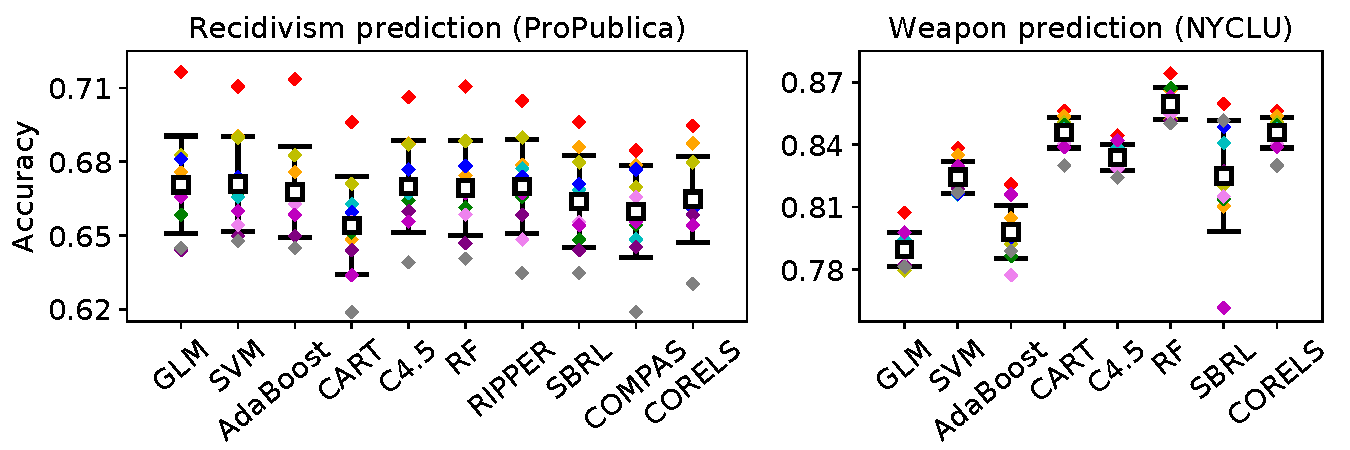
\includegraphics[trim={10mm, 5mm, 25mm, 5mm},
width=0.84\textwidth]{figs/compare-compas-weapon.pdf}
\end{center}
\caption{Comparison of CORELS and a panel of eight other algorithms:
logistic regression~(GLM), support vector machines~(SVM),
AdaBoost, CART, C4.5, random forests~(RF), RIPPER,
scalable Bayesian rule lists~(SBRL).
%
Test accuracy means (white squares),
standard deviations (error bars),
and values (colors correspond to folds),
for 10-fold cross-validation experiments.
%
Left:~Two-year recidivism prediction for the ProPublica COMPAS dataset.
%
For CORELS, we use regularization parameter~${\Reg=0.005}$.
%
Right:~Weapon prediction for the NYCLU stop-and-frisk dataset.
%
For CORELS, we use~${\Reg=0.01}$.
%
Note that we were unable to execute RIPPER for the NYCLU problem.
}
\label{fig:comparison}
\end{figure}

Our experimental analysis addresses five questions:
(1) How does CORELS' accuracy compare to other algorithms?
(2) How does CORELS' model size compare to other algorithms?
(3) How rapidly does the objective function converge?
(4) How rapidly does CORELS prune the search space?
(5) How much does each of the implementation optimizations contribute to CORELS' performance?

\begin{figure}[t!]
\begin{algorithmic}
\State \bif $(location = transit~authority)$ \bthen $yes$
\State \belif $(stop~reason = suspicious~object)$ \bthen $yes$
\State \belif $(stop~reason = suspicious~bulge)$ \bthen $yes$
\State \belse $no$
\end{algorithmic}
\caption{An example rule list that predicts whether a weapon will be found on a
stopped individual who is frisked or searched, for the NYCLU stop-and-frisk dataset.
%
This is the most common optimal rule list found by CORELS across 10 cross-validation
folds; the others contain the same rules, up to a permutation.
}
\label{fig:weapon-rule-list}
\end{figure}

All results that we present were executed on a server with two Intel Xeon E5-2699~v4
(55~MB cache, 2.20~GHz) processors and 448~GB RAM.
%
Except where we mention a memory constraint, all experiments
can run comfortably on smaller machines, \eg a laptop with 16GB~RAM.

Our evaluation focuses on two socially-important prediction problems associated
with recent, publicly-available datasets:
\begin{itemize}
\item Predicting which individuals in the ProPublica COMPAS
dataset~\citep{LarsonMaKiAn16} recidivate within two years.
\item Using the NYCLU 2014 stop-and-frisk dataset~\citep{nyclu:2014} to predict
whether a weapon will be found on a stopped individual who is frisked or searched.
\end{itemize}
%
Our choice of and approach to the second problem is inspired by the work
of~\citet{Goel16}, who develop regression models to analyze racial disparities
in New York City's stop-and-frisk policy, for a similar, larger dataset.
%
In particular, the authors arrive at a simple and interpretable rule that
could potentially be used by police officers to effectively frisk or search
stopped individuals only when these interventions are likely to discover
criminal possession of a weapon.

We first ran a 10-fold cross validation experiment using CORELS and eight other
algorithms:
logistic regression, support vector machines, AdaBoost, CART, C4.5, random forests, RIPPER, and scalable Bayesian rule lists (SBRL).~\footnote{For SBRL, we use the C implementation at \url{https://github.com/Hongyuy/sbrlmod}.}
%
We use standard R packages, with default parameter settings,
for the first seven algorithms.~\footnote{For CART, C4.5 (J48), and RIPPER,
\ie the tree and rule list learning algorithms, we use the implementations
from the R packages rpart, RWeka, and caret, respectively.
%
By default, CART uses complexity parameter ${cp = 0.01}$,
and C4.5 uses complexity parameter ${C = 0.25}$.
}

Figures~\ref{fig:rule-list} and~\ref{fig:weapon-rule-list}
show example optimal rule lists that CORELS learns
for the ProPublica and NYCLU datasets, respectively.
%
While our goal is to provide illustrative examples, and not to provide a
detailed analysis nor to advocate for the use of these specific models,
we note that these rule lists are short and easy to understand.
%
In particular, the three-rule list for weapon prediction
in Figure~\ref{fig:weapon-rule-list} has the spirit of the heuristic
strategy presented by~\citet{Goel16}, that combines three stop criteria
and is based on a reduced version of their full regression model.

Figure~\ref{fig:comparison} shows that there were no statistically significant
differences in algorithm accuracies.
In fact, the difference between folds was far larger than the difference
between algorithms.
We conclude that CORELS produces models whose accuracy is comparable
to those found via other algorithms.

\begin{figure}[t!]
\begin{center}
%\includegraphics[width=0.75\textwidth]{figs/sketch-comparison.png}
% left lower right upper
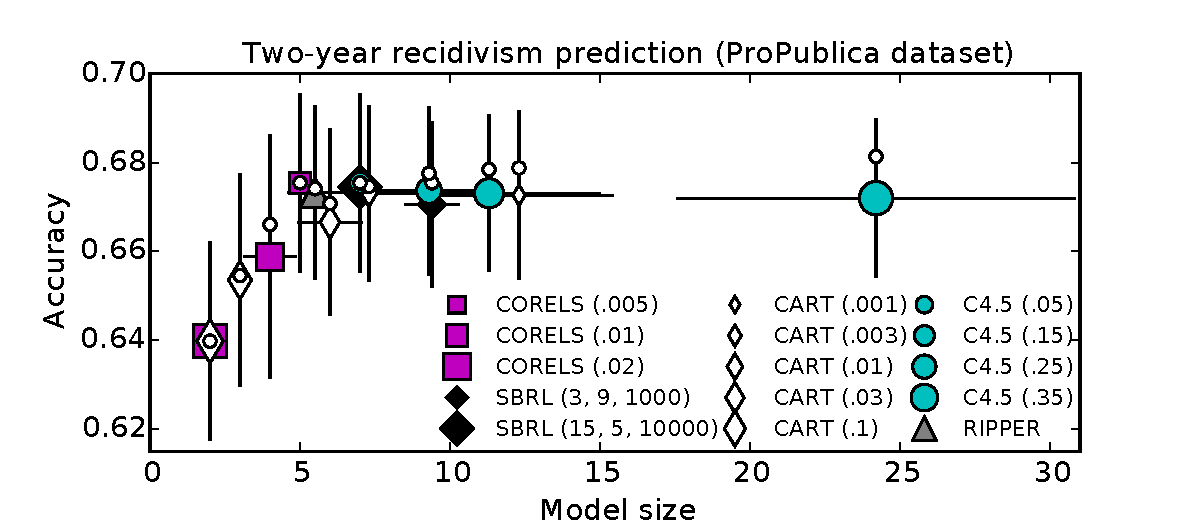
\includegraphics[trim={12mm, 0mm, 24mm, 5mm},
width=0.74\textwidth]{figs/compas-sparsity-training.pdf}
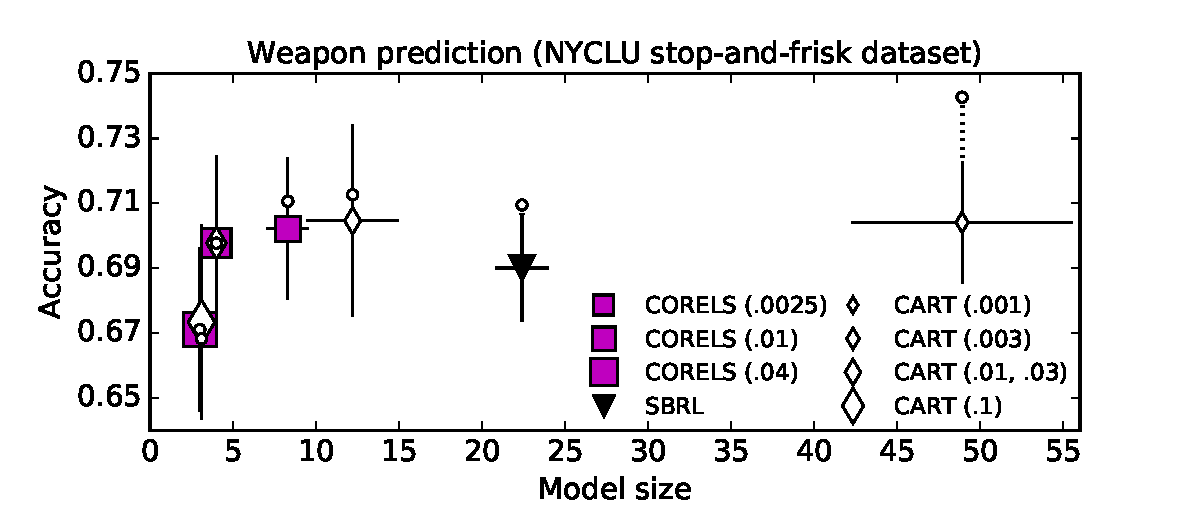
\includegraphics[trim={12mm, 5mm, 24mm, 1mm},
width=0.74\textwidth]{figs/frisk-sparsity-training.pdf}
\end{center}
\caption{Training and test accuracy as a function of model size.
%
For CORELS, CART, and C4.5, we vary the regularization parameter~$\Reg$,
and complexity parameters~$cp$ and~$C$, respectively;
numbers within parentheses in the legend indicate parameter values.
%
Note that the CART implementation sets ${cp = 0.01}$ by default,
and C4.5 uses ${C = 0.25}$.
%
Legend markers and error bars indicate means and standard deviations,
respectively, of test accuracy across cross-validation folds.
%
Small circles mark associated training accuracy means.
%
Top:  Two-year recidivism prediction for the ProPublica COMPAS dataset.
%
None of the models exhibit significant overfitting:
mean training accuracy never exceeds mean test accuracy
by more than about 0.01.
%
Bottom:  Weapon prediction for the NYCLU stop-and-frisk dataset.
%
Only CART with ${cp = 0.001}$ significantly overfits.
%
We do not depict C4.5, which finds large models (${>100}$ leaves)
and dramatically overfits for all tested parameters.
}
\label{fig:sparsity}
\end{figure}

Figure~\ref{fig:sparsity} summarizes differences in accuracy and model size
for CORELS and other tree (CART, C4.5) and rule list (RIPPER, SBRL) learning algorithms.
%
For both problems, CORELS can learn short rule lists without sacrificing accuracy.

\clearpage

\begin{figure}[t!]
\begin{center}
%\includegraphics[width=0.65\textwidth]{figs/sketch-objective.png}
% left lower right upper
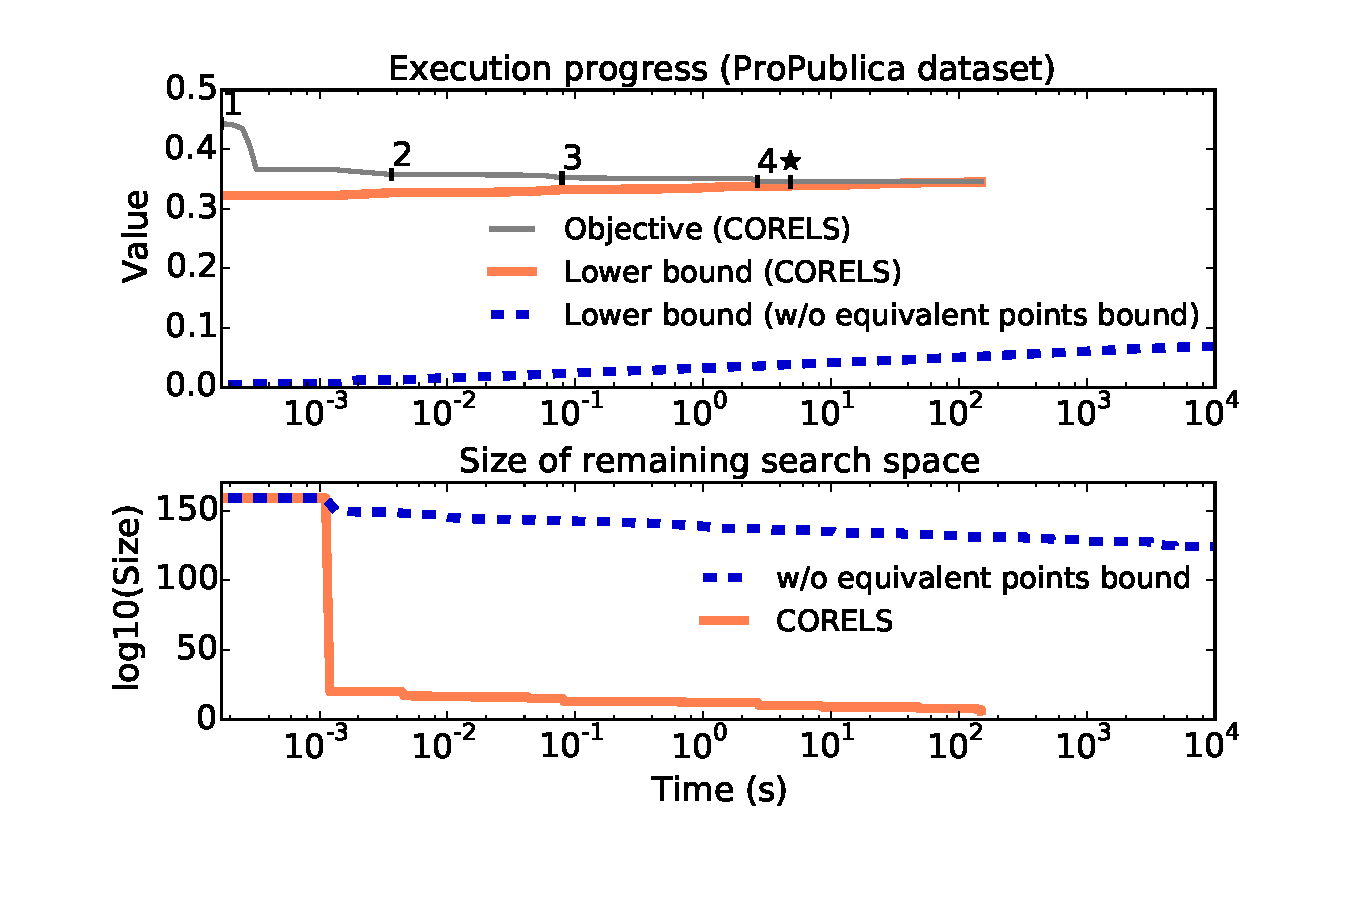
\includegraphics[trim={20mm, 15mm, 24mm, 15mm},
width=0.75\textwidth]{figs/compas_execution-remaining-space.pdf}
\end{center}
\caption{CORELS with (lines) and without
(dashes) the equivalent points bound (Theorem~\ref{thm:identical}).
%
Top: Objective value (thin line) and lower bound (thick line) for CORELS,
as a function of wall clock time (log scale).
%
Numbered hatch marks along the trace of the objective value
indicate when the length of the best known rule list changes,
and are labeled by the new length.
%
CORELS quickly achieves the optimal value (star marker),
and certifies optimality when the lower bound matches the objective value.
%
A separate execution of CORELS without the equivalent points bound remains
far from complete, and its lower bound (dashed line) far from the optimum.
%
Bottom: $\lfloor \log_{10} \Remaining(\CurrentObj, \Queue) \rfloor$,
as a function of wall clock time (log scale),
where~$\Remaining(\CurrentObj, \Queue)$
is the upper bound on remaining search space size
(Theorem~\ref{thm:remaining-eval-fine}).
}
\label{fig:objective}
\end{figure}

In the remainder, we show results using the ProPublica dataset.
%
Figure~\ref{fig:objective} illustrates how both the objective and the size of
the remaining search space decrease as CORELS executes.
The objective drops quickly, achieving the optimal value within 10 seconds.
CORELS certifies optimality in less than 6 minutes --
the objective lower bound of the remaining search space
steadily converges to the optimal objective as the search space shrinks.

Finally, we determine the efficacy of each of our bounds and data structure optimizations.
%
Figure~\ref{fig:objective} highlights how a separate execution of CORELS without
the equivalent points bound remains far from complete,
with its lower bound far from the optimum.
%
Table~\ref{tab:ablation} provides summary statistics for experiments using
the full CORELS implementation and variants each remove a specific optimization.
%
Figure~\ref{fig:queue} presents a view of the same experiments, focusing
on three of our optimizations. These plots depict the number of
prefixes of a given length in the queue during the algorithm's execution.

%\includegraphics[width=0.75\textwidth]{figs/sketch-ablation.png}
\begin{table}[t!]
\centering
\begin{tabular}{l | c | c | c | c | c}
Removed component & $t_\text{total}$ (min) & $t_\text{opt}$ (s) & $i_\text{total}$ ($\times 10^6$) & $Q_\text{max}$ ($\times 10^6$) & $K_\text{max}$ \\
\hline
none (CORELS) & 5.5 (1.6) & 8 (2) & 1.7 (0.4) & 1.3 (0.4) & 5-6 \\
priority queue (BFS) & 6.7 (2.2) & 4 (1) & 1.9 (0.6) & 1.5 (0.5) & 5-6 \\
support bounds & 10.2 (3.4) & 13 (4) & 2.7 (0.8) & 2.2 (0.7) & 5-6 \\
symmetry-aware map & 58.6 (23.3) & 23 (6) & 16.0 (5.9) & 14.5 (5.7) & 5-6 \\
lookahead bound & 71.9 (23.0) & 9 (2) & 18.5 (5.9) & 16.3 (5.3) & 6-7 \\
%equiv. pts. bound & 188.6 (104.6) & 6178 (1840) & 803.8 (0.1) & 790.5 (0.4) & 10-10
equivalent pts bound & $>$134 & $>$7168* & $>$800 & $>$789 & $\ge$10
\end{tabular}
%\vspace{4mm}
\caption{Per-component performance improvement.
%
The columns report total execution time,
time to optimum, number of queue insertions,
maximum queue size, and maximum evaluated prefix length.
%
The first row shows CORELS; subsequent rows show variants
that each remove a specific implementation optimization or bound.
%
(We are not measuring the cumulative effects of removing a sequence of components.)
%
All rows represent complete executions, except for the final row,
in which each execution was terminated due to memory constraints,
once the size of the cache reached ${8 \times 10^8}$ elements,
after consuming 390-410GB RAM.
We terminated each experiment in the last row after consuming 390-410GB RAM.
%
In all but the final row and column, we report means
(and standard deviations) over 10 cross-validation folds;
in the final row, we report the minimum values across folds. \\
%
*~Only 4 out of 10 folds achieve the optimum before being terminated.
}
\vspace{4mm}
\label{tab:ablation}
\end{table}

\begin{figure}[b!]
\begin{center}
% left lower right upper
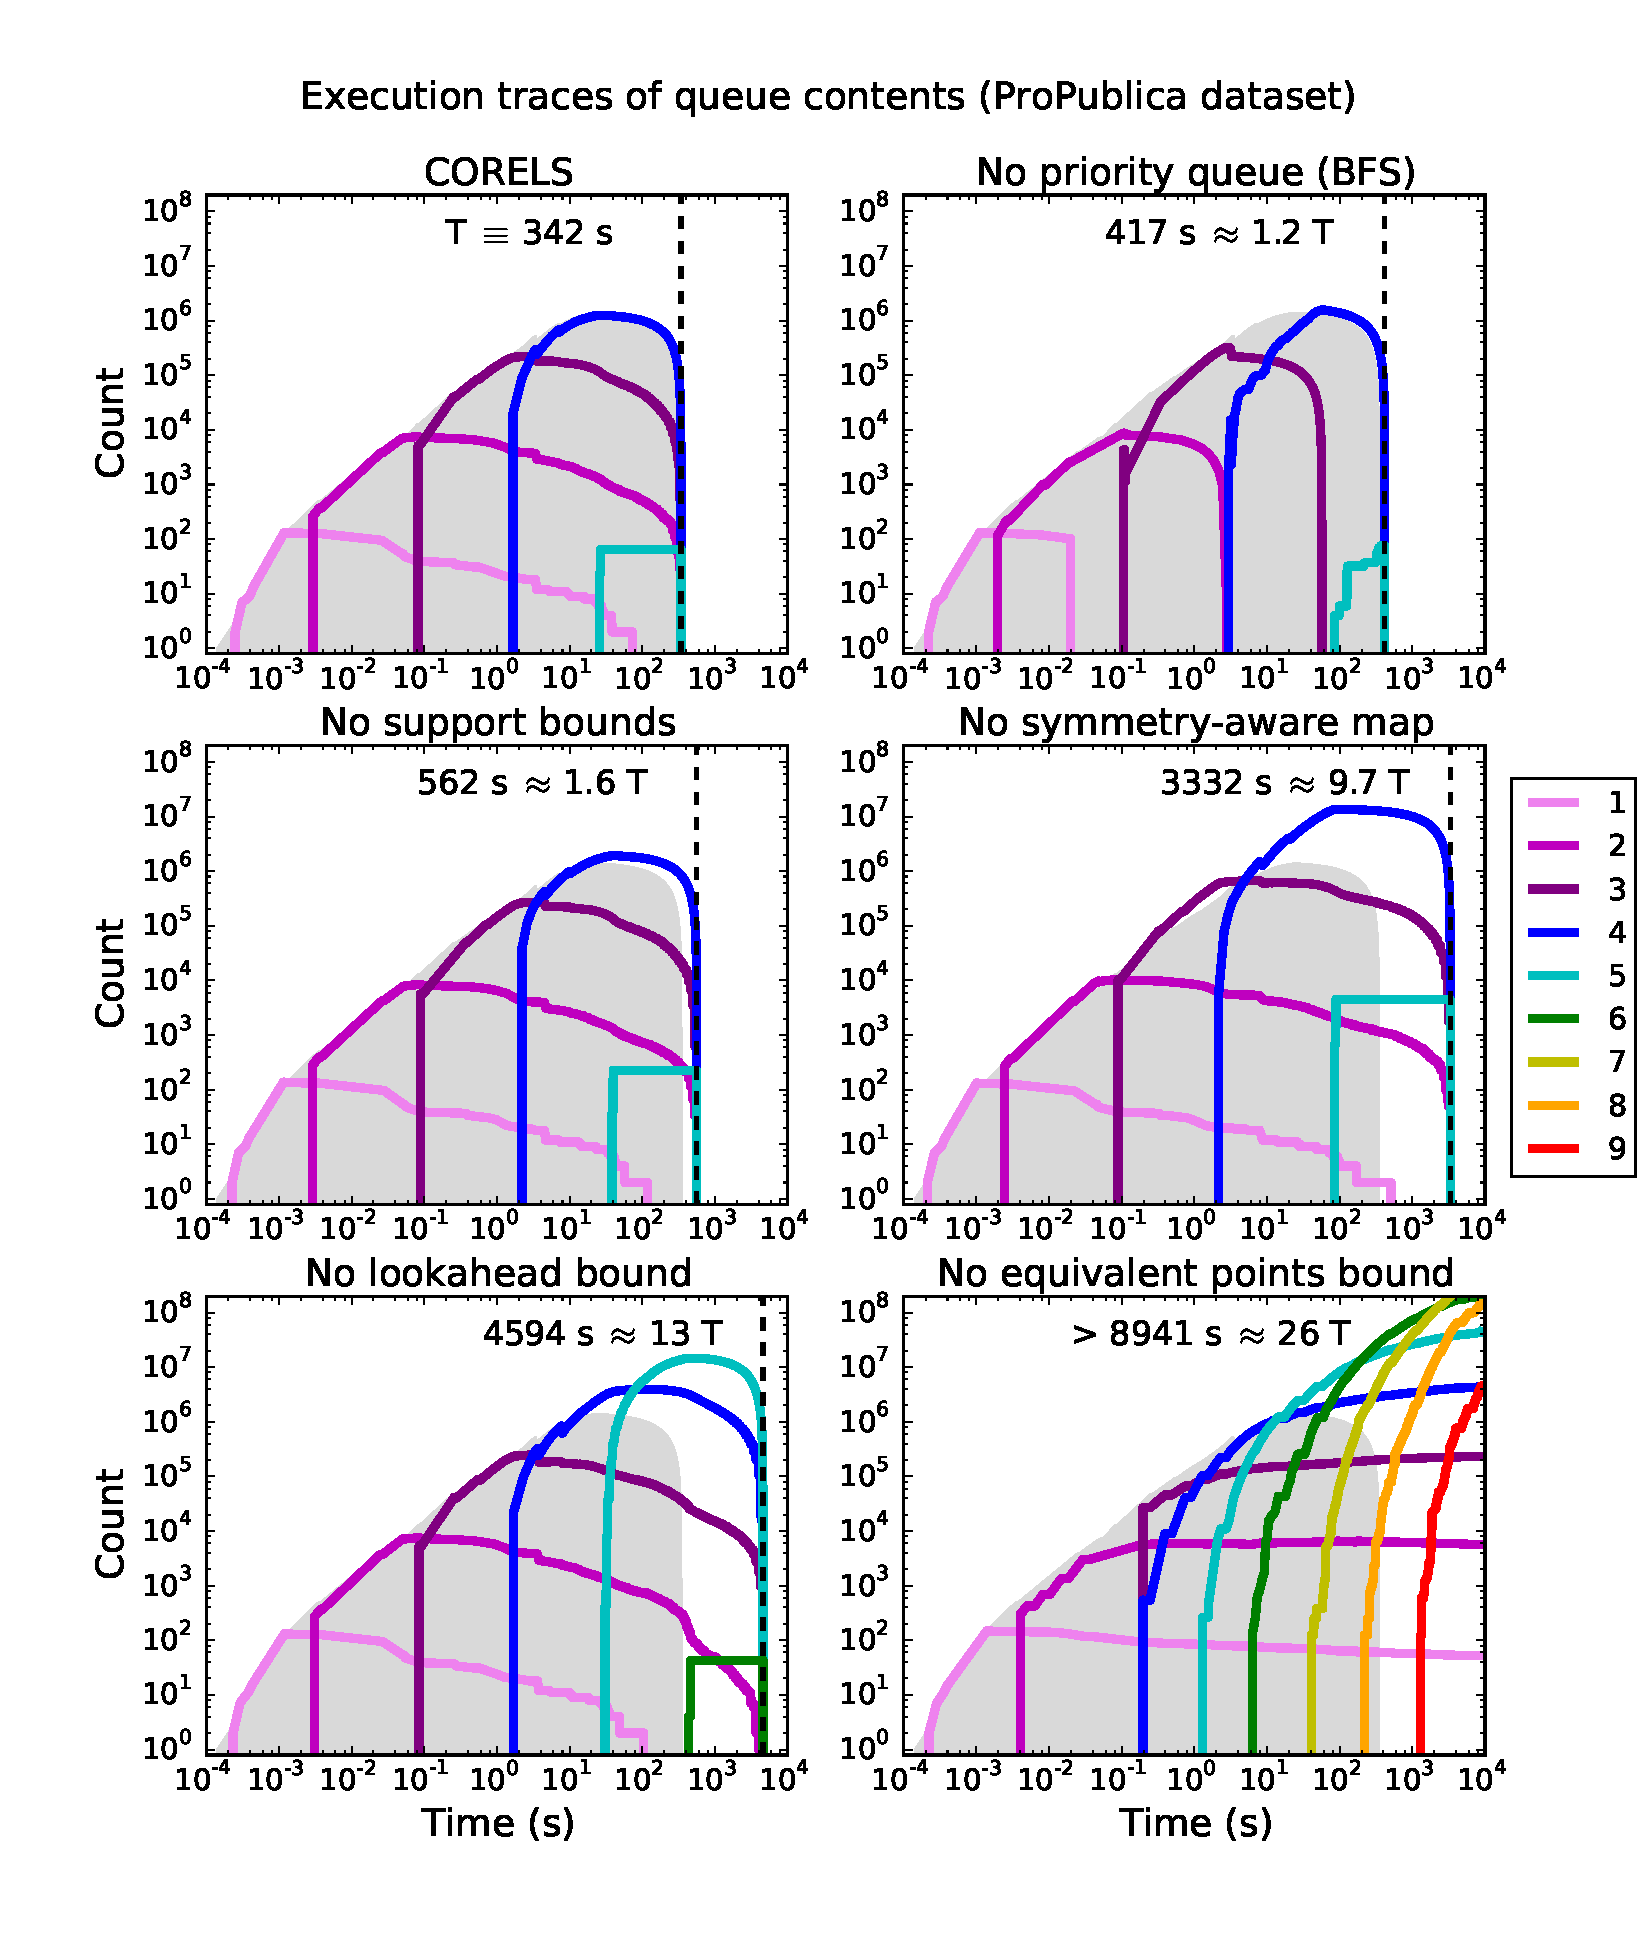
\includegraphics[trim={30mm 10mm 35mm 30mm},
width=0.85\textwidth]{figs/kdd_compas_ablation-queue.pdf}
\end{center}
\caption{Logical queue composition.
%
Numbers of prefixes in the queue (log scale), labeled and colored by length,
as a function of wall clock time (log scale), for CORELS (top left),
and without five specific implementation optimizations or bounds.
%EXPAND HERE
%the permutation bounds (top right),
%lookahead bound (bottom left), and equivalent points bound (bottom right).
%
The gray shading fills in the area beneath the total number of
queue elements for CORELS.
\ie the sum over all lengths in the top left figure.
%
For comparison, we replicate the same gray region
in the other three subfigures.
}
\label{fig:queue}
\end{figure}

\begin{comment}

\begin{table}[t!]
\centering
\begin{tabular}{l | c | c}
Method & ProPublica & NYCLU \\
\hline
CORELS & 67.6 $\pm$ 2.0 & 69.8 $\pm$ 2.7 \\
SBRL & 67.1 $\pm$ 1.7 & 69.7 $\pm$ 2.0 \\
CART & 66.7 $\pm$ 2.1 & 69.8 $\pm$ 2.7 \\
C4.5 & 67.3 $\pm$ 1.8 & 66.8 $\pm$ 2.1 \\
RF & 67.3 $\pm$ 1.8 & 68.7 $\pm$ 2.4 \\
RIPPER & 67.3 $\pm$ 2.0 & --- \\
AdaBoost & 67.3 $\pm$ 1.7 & 70.6 $\pm$ 2.7 \\
GLM & 67.5 $\pm$ 1.8 & 70.3 $\pm$ 2.5 \\
SVM & 67.1 $\pm$ 2.0 & 70.2 $\pm$ 2.7 \\
\end{tabular}
\vspace{5mm}
\caption{Comparison with other methods:
Means and standard deviations of test accuracy.
Also report algorithm runtimes (mean $\pm$ standard deviation over 10 folds).
CORELS ${\Reg = 0.005}$ for ProPublica and ${\Reg = 0.01}$ for NYCLU.}
\label{tab:comparison}
\end{table}

\begin{figure}[t!]
\begin{center}
\end{center}
\caption{Missing:  Some sort of comparison of different scheduling policies}
\label{fig:scheduling-policy}
\end{figure}

\begin{figure}[t!]
\begin{center}
%\includegraphics[width=0.65\textwidth]{figs/sketch-queue-size.png}
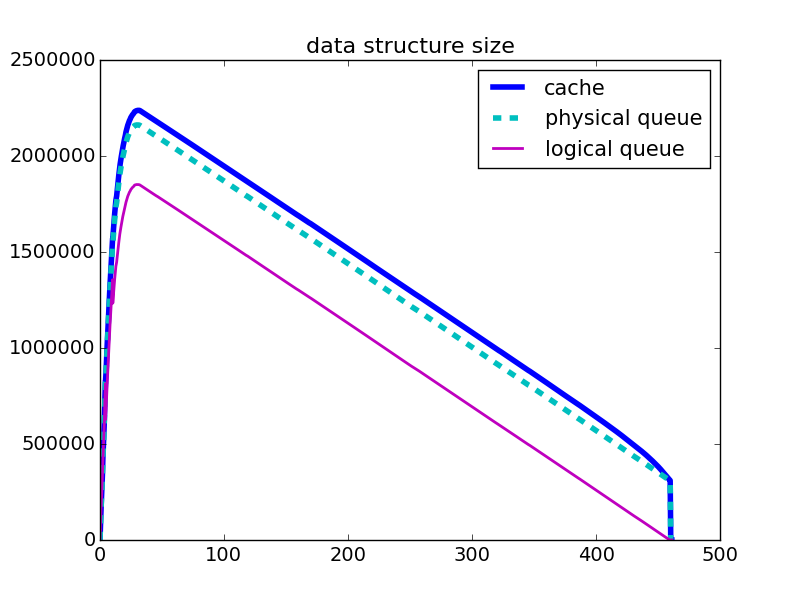
\includegraphics[width=0.8\textwidth]{figs/ela_compas-queue-cache-size-insertions.pdf}
\end{center}
\caption{Cache and queue data structure sizes and insertions.
%
The top plot shows the sizes of the cache and queue data structures,
as a function of wall clock time.
%
The number of nodes in the cache (solid black line) is an
upper bound on the number of elements in the physical queue
(dotted gray line), since the physical queue elements only
correspond to the cache trie data structure's leaf nodes
plus disconnected cache nodes that have been marked for deletion.
%
The queue's physical size is an upper bound on its
logical size (solid blue line), which doesn't include nodes
that have been marked for deletion.
%
The bottom plot shows the cumulative number of cache insertions,
which is equivalent to the cumulative number of queue insertions,
as a function of wall clock time.
}
\label{fig:queue-cache-size-insertions}
\end{figure}

\begin{figure}[t!]
\begin{center}
%\includegraphics[width=0.65\textwidth]{figs/sketch-max-length.png}
\includegraphics[width=0.8\textwidth]{figs/ela-max-length-check.png}
\end{center}
\caption{Max prefix length over time (computed from objective value)}
\label{fig:max-length}
\end{figure}

\begin{figure}[t!]
\begin{center}
\includegraphics[width=0.8\textwidth]{figs/ela_compas-prefix-length.pdf}
\end{center}
\caption{Best prefix length over time}
\label{fig:prefix-length}
\end{figure}
\end{comment}


\section{Conclusion}

CORELS is an efficient and accurate algorithm for constructing provably optimal rule lists.
%
Optimality is particularly important in domains where model interpretability
has social consequences, \eg recidivism prediction.
%
While achieving optimality on such discrete optimization problems is
computationally hard in general, we aggressively prune our problem's search space
via a suite of bounds.
%
This makes realistically sized problems tractable.
%
CORELS is amenable to parallelization, which should allow it to scale to
even larger problems.

\begin{arxiv}
Finally, we would like to clarify some limitations of CORELS.
%
As far as we can tell, CORELS is the current best algorithm for solving a
specialized optimal decision tree problem.
%
While our approach scales well to large numbers of observations,
it could have difficulty proving optimality
for problems with many possibly relevant features that are highly correlated,
when large regions of the search space might be challenging to exclude.

CORELS is not designed for raw image processing or other problems where the features
themselves are not interpretable.
%
It also does not automatically choose the subgroup with the highest likelihood of a
positive outcome; doing so would require an algorithm such as Falling Rule Lists \citep{WangRu15},
which forces the estimated probabilities to decrease along the list.
%
While CORELS does not technically produce estimates of ${\P(Y=1 \given x)}$,
one could form such an estimate by computing the empirical
proportion ${\hat{\P}(Y=1 \given x \textrm{ obeys } p_k)}$ for each antecedent~$p_k$.
%
Furthermore, it is not designed to assist with causal inference applications, since
it does not estimate the effect of a treatment via the conditional difference
${\P(Y=1 \given \textrm{treatment} = \textrm{True}, x) -}$ ${\P(Y=1 \given \textrm{treatment} = \textrm{False}, x)}$.
%
Alternative algorithms that estimate conditional differences with interpretable
rule lists include Causal Falling Rule Lists \citep{WangRu16}
and Cost-Effective Interpretable Treatment Regimes (CITR) \citep{LakkarajuRu17}.

Lastly, recall that a rule list is a form of decision tree,
where in our setting, the leaves are conjunctions.
%
It may be possible to generalize ideas from CORELS to handle decision trees of
other forms, which could be an interesting project for future work.
\end{arxiv}


% Acknowledgements should go at the end, before appendices and references
\acks{E.A. is supported by the Miller Institute for Basic Research in Science,
University of California, Berkeley, and is hosted by Prof. M.I. Jordan at RISELab.
%
C.D.R. is supported in part by MIT-Lincoln Labs.
%
E.A. would like to thank E. Jonas, E. Kohler, and S. Tu for early implementation
guidance, A.~D'Amour for pointing out the work by~\citet{Goel16},
J.~Schleier-Smith and E.~Thewalt for helpful conversations, and members of RISELab,
SAIL, and the UC Berkeley Database Group for their support and feedback.
%
We thank H.~Yang and B.~Letham for sharing advice and code for processing data
and mining rules.
}

\vskip 0.2in
\bibliography{refs}

\renewcommand{\theHsection}{A\arabic{section}}
\appendix
%\renewcommand{\thesection}{\Alph{section}}
\newpage
\section{Excessive antecedent support}
\label{appendix:ub-supp}

\begin{theorem}[Upper bound on antecedent support]
\label{thm:ub-support}
Let ${\OptimalRL = (\Prefix, \Labels, \Default, K)}$
be any optimal rule list with objective~$\OptimalObj$, \ie
${\OptimalRL \in \argmin_\RL \Obj(\RL, \x, \y)}$,
and let ${\Prefix = (p_1, \dots, p_{k-1},}$
${p_k, \dots, p_K)}$ be its prefix.
%
For each ${k \le K}$, antecedent~$p_k$ in~$\Prefix$
has support less than or equal to
the fraction of all data not captured by preceding antecedents,
by an amount greater than the regularization parameter~$\Reg$:
\begin{align}
\Supp(p_k, \x \given \Prefix) \le 1 - \Supp(\Prefix^{k-1}, \x) - \Reg,
\label{eq:ub-support}
\end{align}
where ${\Prefix^{k-1} = (p_1, \dots, p_{k-1})}$.
%
For the last antecedent, \ie when ${p_k = p_K}$, equality implies
that there also exists a shorter optimal rule list
${\RL' = (\Prefix^{K-1}, \Labels', \Default', K - 1) \in}$ ${\argmin_\RL \Obj(\RL, \x, \y)}$.
%with prefix~$\Prefix^{K-1}$.
\end{theorem}

\begin{proof}
First, we focus on the last antecedent~$p_{K+1}$ in a rule list~$\RL'$.
%
Let ${\RL = (\Prefix, \Labels, \Default, K)}$
be a rule list with prefix ${\Prefix = (p_1, \dots, p_K)}$
and objective ${\Obj(\RL, \x, \y) \ge \OptimalObj}$, where
${\OptimalObj \equiv}$ ${\min_{\RLB} \Obj(\RLB, \x, \y)}$
is the optimal objective.
%
Let ${\RL' = (\Prefix', \Labels', \Default', K + 1)}$
be a rule list whose prefix ${\Prefix' = (p_1, \dots, p_K, p_{K+1})}$
starts with~$\Prefix$ and ends with a new antecedent~$p_{K+1}$.
%
Suppose~$p_{K+1}$ in the context of~$\Prefix'$ captures nearly all
data not captured by~$\Prefix$, except for a fraction~$\epsilon$
upper bounded by the regularization parameter~$\Reg$:
\begin{align*}
1 - \Supp(\Prefix, \x) - \Supp(p_{K+1}, \x \given \Prefix') \equiv \epsilon \le \Reg.
\end{align*}
%
Since~$\Prefix'$ starts with~$\Prefix$,
its prefix misclassification error is at least as great;
the only discrepancy between the misclassification errors
of~$\RL$ and~$\RL'$ can come from the difference between the support of
the set of data not captured by~$\Prefix$ and the support of~$p_{K+1}$:
\begin{align*}
| \Loss(\RL', \x, \y) - \Loss(\RL, \x, \y) | \le
1 - \Supp(\Prefix, \x) - \Supp(p_{K+1}, \x \given \Prefix') = \epsilon.
\end{align*}
The best outcome for~$\RL'$ would occur if its misclassification
error were smaller than that of~$\RL$ by~$\epsilon$,
%\eg this could happen if all data not captured by~$\Prefix'$
%had the same class label, in which case the default rule of~$\RL'$
%would incur zero misclassification error.
% --> it's more complicated, would need to discuss minority class label, etc.
%
therefore
\begin{align*}
\Obj(\RL', \x, \y) &= \Loss(\RL', \x, \y) + \Reg (K+1) \\
&\ge \Loss(\RL, \x, \y) - \epsilon + \Reg(K+1)
= \Obj(\RL, \x, \y) - \epsilon + \Reg \ge \Obj(\RL, \x, \y) \ge \OptimalObj.
\end{align*}
$\RL'$ is an optimal rule list,
\ie ${\RL' \in \argmin_{\RLB} \Obj(\RLB, \x, y)}$,
if and only if ${\Obj(\RL', \x, \y) = \Obj(\RL, \x, \y) =}$ ${\OptimalObj}$,
which requires ${\epsilon = \Reg}$.
%
Otherwise, ${\epsilon < \Reg}$, in which case
\begin{align*}
\Obj(\RL', \x, \y) \ge \Obj(\RL, \x, \y) - \epsilon + \Reg
> \Obj(\RL, \x, \y) \ge \OptimalObj,
\end{align*}
therefore $\RL'$ is not optimal, \ie  ${\RL' \notin \argmin_{\RLB} \Obj(\RLB, \x, \y)}$.
%
This demonstrates the desired result for ${k = K}$.

In the remainder, we prove the bound in~\eqref{eq:ub-support} by contradiction,
in the context of a rule list~$\RL''$.
%
Let~$\RL$ and~$\RL'$ retain their definitions from above,
thus as before, that the data not captured by~$\Prefix'$
has normalized support~${\epsilon \le \Reg}$, \ie
\begin{align*}
1 - \Supp(\Prefix', \x) = 1 - \Supp(\Prefix, \x) - \Supp(p_{K+1}, \x \given \Prefix') = \epsilon \le \Reg.
\end{align*}
Thus for any rule list~$\RL''$ whose prefix
$\Prefix'' = (p_1, \dots, p_{K+1}, \dots, p_{K'})$ starts
with~$\Prefix'$ and ends with one or more additional rules,
each additional rule~$p_k$ has support
${\Supp(p_k, \x \given \Prefix'') \le}$ ${\epsilon \le \Reg}$,
for all~${k > K+1}$.
%
By Theorem~\ref{thm:min-capture},
all of the additional rules have insufficient support,
therefore~$\Prefix''$ cannot be optimal,
\ie ${\RL'' \notin \argmin_{\RLB} \Obj(\RLB, \x, \y)}$.
\end{proof}

Similar to Theorem~\ref{thm:min-capture}, our lower bound on
antecedent support, we can apply Theorem~\ref{thm:ub-support}
in the contexts of both constructing rule lists and
rule mining~(\S\ref{sec:setup}).
%
Theorem~\ref{thm:ub-support} implies that if we only seek a single
optimal rule list, then during branch-and-bound execution,
we can prune a prefix if we ever add an antecedent with support
too similar to the support of the set of data not captured by the
preceding antecedents.
%
One way to view this result is that if
${\RL = (\Prefix, \Labels, \Default, K)}$
and ${\RL' = (\Prefix', \Labels', \Default', K + 1)}$
are rule lists such that~$\Prefix'$ starts with~$\Prefix$
and ends with an antecedent that captures all or nearly all
data not captured by~$\Prefix$, then the new rule in~$\RL'$
behaves similar to the default rule of~$\RL$.
%
As a result, the misclassification error of~$\RL'$ must be
similar to that of~$\RL$, and any reduction may not be
sufficient to offset the penalty for longer prefixes.

\begin{proposition}[Excessive antecedent support propagates]
\label{prop:ub-support}
Define~$\StartContains(\Prefix)$ as in~\eqref{eq:start-contains},
and let ${\Prefix = (p_1, \dots, p_{K})}$ be a prefix,
such that its last antecedent~$p_{K}$ has excessive support,
\ie the opposite of the bound in~\eqref{eq:ub-support}:
\begin{align*}
\Supp(p_K, \x \given \Prefix) > 1 - \Supp(\Prefix^{K-1}, \x) - \Reg,
\end{align*}
where ${\Prefix^{K-1} = (p_1, \dots, p_{K-1})}$.
%
Let ${\RLB = (\PrefixB, \LabelsB, \DefaultB, \kappa)}$
be any rule list with prefix
${\PrefixB =}$ ${(P_1, \dots, P_{\kappa})}$
such that~$\PrefixB$ starts with ${\PrefixB^{K'-1} =}$
${(P_1, \dots, P_{K'-1}) \in \StartContains(\Prefix^{K-1})}$
and~${P_{K'} = p_{K}}$.
%
It follows that~$P_{K'}$ has excessive support in prefix~$\PrefixB$,
and furthermore, ${\RLB \notin \argmin_{\RL} \Obj(\RL, \x, \y)}$.
\end{proposition}

\begin{proof}
Since ${\PrefixB^{K'} = (P_1, \dots, P_{K'})}$
contains all the antecedents in~$\Prefix$, we have that
\begin{align*}
\Supp(\PrefixB^{K'}, \x) \ge \Supp(\Prefix, \x).
\end{align*}
Expanding these two terms gives
\begin{align*}
\Supp(\PrefixB^{K'}, \x)
&= \Supp(\PrefixB^{K'-1}, \x) + \Supp(P_{K'}, \x \given \PrefixB) \\
&\ge \Supp(\Prefix, \x)
= \Supp(\Prefix^{K-1}, \x) + \Supp(p_K, \x \given \Prefix)
> 1 - \Reg.
\end{align*}
Rearranging gives
\begin{align*}
\Supp(P_{K'}, \x \given \PrefixB)
> 1 - \Supp(\PrefixB^{K'-1}, \x) - \Reg,
\end{align*}
thus~$P_{K'}$ has excessive support in~$\PrefixB$.
%
By Theorem~\ref{thm:ub-support},
${\RLB \notin \argmin_{\RL} \Obj(\RL, \x, \y)}$.
\end{proof}

\section{Proof of Theorem~\ref{thm:equivalent} (Equivalent support bound)}
\label{appendix:equiv-supp}

We begin by defining four related rule lists.
%
First, let ${\RL = (\Prefix, \Labels, \Default, K)}$
be a rule list with prefix ${\Prefix = (p_1, \dots, p_K)}$
and labels ${\Labels = (q_1, \dots, q_K)}$.
%
Second, let ${\RLB = (\PrefixB, \LabelsB, \DefaultB, \kappa)}$
be a rule list with prefix ${\PrefixB = (P_1, \dots, P_\kappa)}$
that captures the same data as~$\Prefix$,
and labels ${\LabelsB = (Q_1, \dots, Q_\kappa)}$.
%
Third, let ${\RL' = (\Prefix', \Labels', \Default', K') \in}$
${\StartsWith(\Prefix)}$ be any rule list
whose prefix starts with~$\Prefix$, such that~${K' \ge K}$.
%
Denote the prefix and labels of~$\RL'$ by
${\Prefix' = (p_1, \dots, p_K,}$ ${p_{K+1}, \dots, p_{K'})}$
and ${\Labels = (q_1, \dots, q_{K'})}$, respectively.
%
Finally, define ${\RLB' = (\PrefixB', \LabelsB', \DefaultB', \kappa') \in}$
${\StartsWith(\PrefixB)}$ to be the `analogous' rule list, \ie whose prefix
${\PrefixB' = (P_1, \dots, P_\kappa, P_{\kappa+1}, \dots, P_{\kappa'}) =}$
${(P_1, \dots, P_\kappa, p_{K+1}, \dots, p_{K'})}$
starts with~$\PrefixB$ and ends with the same ${K'-K}$
antecedents as~$\Prefix'$.
%
Let ${\LabelsB' = (Q_1, \dots, Q_{\kappa'})}$
denote the labels of~$\RLB'$.

Next, we claim that the difference in the objectives
of rule lists~$\RL'$ and~$\RL$ is the same as the difference
in the objectives of rule lists~$\RLB'$ and~$\RLB$.
%
Let us expand the first difference as
\begin{align}
&\Obj(\RL', \x, \y) - \Obj(\RL, \x, \y)
  = \Loss(\RL', \x, \y) + \Reg K' - \Loss(\RL, \x, \y) - \Reg K \nn \\
&= \Loss_p(\Prefix', \Labels', \x, \y) + \Loss_0(\Prefix', \Default', \x, \y)
  - \Loss_p(\Prefix, \Labels, \x, \y) - \Loss_0(\Prefix, \Default, \x, \y)
  + \Reg (K' - K). \nn
\end{align}
Similarly, let us expand the second difference as
\begin{align}
&\Obj(\RLB', \x, \y) - \Obj(\RLB, \x, \y)
  = \Loss(\RLB', \x, \y) + \Reg \kappa' - \Loss(\RLB, \x, \y) - \Reg \kappa \nn \\
&= \Loss_p(\PrefixB', \LabelsB', \x, \y) + \Loss_0(\PrefixB', \DefaultB', \x, \y)
  - \Loss_p(\PrefixB, \LabelsB, \x, \y) - \Loss_0(\PrefixB, \DefaultB, \x, \y)
  + \Reg (K' - K), \nn
\end{align}
where we have used the fact that ${\kappa' - \kappa = K' - K}$.

The prefixes~$\Prefix$ and~$\PrefixB$ capture the same data.
%
Equivalently, the set of data that is not captured by~$\Prefix$
is the same as the set of data that is not captured by~$\PrefixB$, \ie
\begin{align}
\{x_n : \neg\, \Cap(x_n, \Prefix)\} = \{x_n : \neg\, \Cap(x_n, \PrefixB)\}. \nn
\end{align}
Thus, the corresponding rule lists~$\RL$ and~$\RLB$
share the same default rule, \ie ${\Default = \DefaultB}$,
yielding the same default rule misclassification error:
\begin{align}
\Loss_0(\Prefix, \Default, \x, \y) = \Loss_0(\PrefixB, \DefaultB, \x, \y). \nn
\end{align}
Similarly, prefixes~$\Prefix'$ and~$\PrefixB'$ capture
the same data, and thus rule lists~$\RL'$ and~$\RLB'$
have the same default rule misclassification error:
\begin{align}
\Loss_0(\Prefix, \Default, \x, \y) = \Loss_0(\PrefixB, \DefaultB, \x, \y). \nn
\end{align}

At this point, to demonstrate our claim relating the objectives
of~$\RL$, $\RL'$, $\RLB$, and~$\RLB'$, what remains is to
show that the difference in the misclassification errors
of prefixes~$\Prefix'$ and~$\Prefix$ is the same as that
between~$\PrefixB'$ and~$\PrefixB$.
%
We can expand the first difference as
\begin{align}
\Loss_p(\Prefix', \Labels', \x, \y) - \Loss_p(\Prefix, \Labels, \x, \y)
%&= \frac{1}{N} \sum_{n=1}^N \sum_{k=1}^{K'}
%  \one [ \Cap(x_n, p_k \given \Prefix') \wedge (q_k \neq y_n) ]
%  - \frac{1}{N} \sum_{n=1}^N \sum_{k=1}^K
%  \one [ \Cap(x_n, p_k \given \Prefix) \wedge (q_k \neq y_n) ] \\
&= \frac{1}{N} \sum_{n=1}^N \sum_{k=K+1}^{K'}
  \Cap(x_n, p_k \given \Prefix') \wedge \one [ q_k \neq y_n ], \nn
\end{align}
where we have used the fact that since~$\Prefix'$
starts with~$\Prefix$, the first~$K$ rules in~$\Prefix'$
make the same mistakes as those in~$\Prefix$.
%
Similarly, we can expand the second difference as
\begin{align}
\Loss_p(\PrefixB', \LabelsB', \x, \y) - \Loss_p(\PrefixB, \LabelsB, \x, \y)
&= \frac{1}{N} \sum_{n=1}^N \sum_{k=\kappa+1}^{\kappa'}
  \Cap(x_n, P_k \given \PrefixB') \wedge \one [ Q_k \neq y_n ] \nn \\
&= \frac{1}{N} \sum_{n=1}^N \sum_{k=K+1}^{K'}
  \Cap(x_n, p_k \given \PrefixB') \wedge \one [ Q_k \neq y_n ] \nn \\
&= \frac{1}{N} \sum_{n=1}^N \sum_{k=K+1}^{K'}
  \Cap(x_n, p_k \given \Prefix') \wedge \one [ q_k \neq y_n ] \label{eq:third} \\
&= \Loss_p(\Prefix', \Labels', \x, \y) - \Loss_p(\Prefix, \Labels, \x, \y) \nn.
\end{align}
To justify the equality in~\eqref{eq:third}, we observe first that
prefixes~$\PrefixB'$ and~$\Prefix'$ start with~$\kappa$ and~$K$
antecedents, respectively, that capture the same data.
%
Second, prefixes~$\PrefixB'$ and~$\Prefix'$ end with exactly
the same ordered list of~${K' - K}$ antecedents,
therefore for any~${k = 1, \dots, K' - K}$,
antecedent ${P_{\kappa + k} = p_{K + k}}$ in~$\PrefixB'$
captures the same data as~$p_{K + k}$ captures in~$\Prefix'$.
%
It follows that the corresponding labels are all equivalent, \ie
${Q_{\kappa + k} = q_{K + k}}$, for all~${k = 1, \dots, K' - K}$,
and consequently, the prefix misclassification error associated
with the last~${K' - K}$ antecedents of~$\Prefix'$ is the same
as that of~$\PrefixB'$.
%
We have therefore shown that the difference between the objectives
of~$\RL'$ and~$\RL$ is the same as that between~$\RLB'$ and~$\RLB$, \ie
\begin{align}
\Obj(\RL', \x, \y) - \Obj(\RL, \x, \y)
= \Obj(\RLB', \x, \y) - \Obj(\RLB, \x, \y).
\label{eq:equiv-analogous}
\end{align}

Next, suppose that the objective lower bounds of~$\RL$ and~$\RLB$
obey ${b(\Prefix, \x, \y) \le b(\PrefixB, \x, \y)}$, therefore
\begin{align}
\Obj(\RL, \x, \y)
&= \Loss_p(\Prefix, \Labels, \x, \y) + \Loss_0(\Prefix, \Default, \x, \y) + \Reg K \nn \\
&= b(\Prefix, \x, \y) + \Loss_0(\Prefix, \Default, \x, \y) \nn \\
&\le b(\PrefixB, \x, \y) + \Loss_0(\Prefix, \Default, \x, \y)
= b(\PrefixB, \x, \y) + \Loss_0(\PrefixB, \DefaultB, \x, \y)
= \Obj(\RLB, \x, \y).
\label{eq:equiv-ineq}
\end{align}
Now let~$\RL^*$ be an optimal rule list with prefix
constrained to start with~$\Prefix$,
\begin{align}
\RL^* \in \argmin_{\RL^\dagger \in \StartsWith(\Prefix)} \Obj(\RL^\dagger, \x, \y), \nn
\end{align}
and let~$K^*$ be the length of~$\RL^*$.
%
Let~$\RLB^*$ be the analogous $\kappa^*$-rule list whose prefix starts
with~$\PrefixB$ and ends with the same~${K^* - K}$ antecedents as~$\RL^*$,
where~${\kappa^* = \kappa + K^* - K}$.
%
By~\eqref{eq:equiv-analogous},
\begin{align}
\Obj(\RL^*, \x, \y) - \Obj(\RL, \x, \y)
= \Obj(\RLB^*, \x, \y) - \Obj(\RLB, \x, \y).
\label{eq:equiv-diff}
\end{align}
Furthermore, we claim that~$\RLB^*$ is an optimal rule list
with prefix constrained to start with~$\PrefixB$,
\begin{align}
\RLB^* \in \argmin_{\RLB^\dagger \in \StartsWith(\PrefixB)} \Obj(\RLB^\dagger, \x, \y).
\label{eq:equiv-analogous-optimal}
\end{align}

To demonstrate~\eqref{eq:equiv-analogous-optimal},
we consider two separate scenarios.
%
In the first scenario, prefixes~$\Prefix$ and~$\PrefixB$
are composed of the same antecedents,
\ie the two prefixes are equivalent up to a permutation of
their antecedents, and as a consequence,
${\kappa = K}$ and~${\kappa^* = K^*}$.
%
Here, every rule list~${\RL'' \in \StartsWith(\Prefix)}$
that starts with~$\Prefix$
has an analogue~${\RLB'' \in \StartsWith(\PrefixB)}$
that starts with~$\PrefixB$,
such that~$\RL''$ and~$\RLB''$ obey~\eqref{eq:equiv-analogous},
and vice versa, and thus~\eqref{eq:equiv-analogous-optimal}
is a direct consequence of~\eqref{eq:equiv-diff}.

In the second scenario, prefixes~$\Prefix$ and~$\PrefixB$
are not composed of the same antecedents.
%
Define~${\phi = \{p_k : (p_k \in \Prefix) \wedge (p_k \notin \PrefixB)\}}$
to be the set of antecedents in~$\Prefix$ that are not in~$\PrefixB$,
and define~${\Phi = \{P_k : (P_k \in \PrefixB) \wedge (P_k \notin \Prefix)\}}$
to be the set of antecedents in~$\PrefixB$ that are not in~$\Prefix$;
either~${\phi \neq \emptyset}$, or~${\Phi \neq \emptyset}$, or both.

Suppose~${\phi \neq \emptyset}$, and let~${p \in \phi}$
be an antecedent in~$\phi$.
%
It follows that there exists a subset of rule lists
in~$\StartsWith(\PrefixB)$ that do not have analogues
in~$\StartsWith(\Prefix)$.
%
Let~${\RLB'' \in \StartsWith(\PrefixB)}$ be such a rule list,
such that its prefix ${\PrefixB'' = (P_1, \dots, P_\kappa, \dots, p, \dots)}$
starts with~$\PrefixB$ and contains~$p$ among its remaining antecedents.
%
Since~$p$ captures a subset of the data that~$\Prefix$ captures,
and~$\PrefixB$ captures the same data as~$\Prefix$,
it follows that~$p$ does not capture any data in~$\PrefixB''$, \ie
\begin{align}
\frac{1}{N} \sum_{n=1}^N \Cap(x_n, p \given \PrefixB'') = 0 \le \Reg. \nn
\end{align}
By Theorem~\ref{thm:min-capture}, antecedent~$p$ has insufficient
support in~$\RLB''$, and thus~$\RLB''$ cannot be optimal, \ie
${\RLB'' \notin}$ ${\argmin_{\RLB^\dagger \in \StartsWith(\PrefixB)} \Obj(\RLB^\dagger, \x, \y)}$.
%
By a similar argument, if~${\Phi \neq \emptyset}$
and~${P \in \Phi}$, and~${\RL'' \in \StartsWith(\Prefix)}$
is any rule list whose prefix starts with~$\Prefix$
and contains antecedent~$P$, then~$\RL''$ cannot be optimal, \ie
${\RL'' \notin \argmin_{\RL^\dagger \in \StartsWith(\Prefix)} \Obj(\RL^\dagger, \x, \y)}$.

To finish justifying claim~\eqref{eq:equiv-analogous-optimal}
for the second scenario, first define
\begin{align}
\tau(\Prefix, \Phi) \equiv
  \{\RL'' = (\Prefix'', \Labels'', \Default'', K'') :
    \RL'' \in \StartsWith(\Prefix) \textnormal{ and }
    p_k \notin \Phi, \forall p_k \in \Prefix''\} \subset \StartsWith(\Prefix) \nn
\end{align}
to be the set of all rule lists whose prefixes start with~$\Prefix$
and do not contain any antecedents in~$\Phi$.
%
Now, recognize that the optimal prefixes in~$\tau(\Prefix, \Phi)$
and~$\StartsWith(\Prefix)$ are the same, \ie
\begin{align}
\argmin_{\RL^\dagger \in \tau(\Prefix, \Phi)} \Obj(\RL^\dagger, \x, \y)
= \argmin_{\RL^\dagger \in \StartsWith(\Prefix)} \Obj(\RL^\dagger, \x, \y), \nn
\end{align}
and similarly, the optimal prefixes in~$\tau(\PrefixB, \phi)$
and~$\StartsWith(\PrefixB)$ are the same, \ie
\begin{align}
\argmin_{\RLB^\dagger \in \tau(\PrefixB, \phi)} \Obj(\RLB^\dagger, \x, \y)
= \argmin_{\RLB^\dagger \in \StartsWith(\PrefixB)} \Obj(\RLB^\dagger, \x, \y). \nn
\end{align}
Since we have shown that every~${\RL'' \in \tau(\Prefix, \Phi)}$
has a direct analogue~${\RLB'' \in \tau(\PrefixB, \phi)}$,
such that~$\RL''$ and~$\RLB''$ obey~\eqref{eq:equiv-analogous},
and vice versa, we again have~\eqref{eq:equiv-analogous-optimal}
as a consequence of~\eqref{eq:equiv-diff}.

We can now finally combine~\eqref{eq:equiv-ineq}
and~\eqref{eq:equiv-analogous-optimal} to obtain the desired inequality in~\eqref{eq:equivalent}:
\begin{align}
\min_{\RL' \in \StartsWith(\Prefix)} \Obj(\RL', \x, \y)
= \Obj(\RL^*, \x, \y) \le \Obj(\RLB^*, \x, \y)
= \min_{\RLB' \in \StartsWith(\PrefixB)} \Obj(\RLB', \x, \y). \nn
\end{align}

\section{Proof of Theorem~\ref{thm:similar} (Similar support bound)}
\label{appendix:similar-supp}

We begin by defining four related rule lists.
%
First, let ${\RL = (\Prefix, \Labels, \Default, K)}$
be a rule list with prefix ${\Prefix = (p_1, \dots, p_K)}$
and labels ${\Labels = (q_1, \dots, q_K)}$.
%
Second, let ${\RLB = (\PrefixB, \LabelsB, \DefaultB, \kappa)}$
be a rule list with prefix ${\PrefixB = (P_1, \dots, P_\kappa)}$
and labels ${\LabelsB = (Q_1, \dots, Q_\kappa)}$.
%
Define~$\omega$ as in~\eqref{eq:omega}
and~$\Omega$ as in~\eqref{eq:big-omega},
and require that~${\omega, \Omega \le \Reg}$.
%
Third, let ${\RL' = (\Prefix', \Labels', \Default', K') \in}$
${\StartsWith(\Prefix)}$ be any rule list
whose prefix starts with~$\Prefix$, such that~${K' \ge K}$.
%
Denote the prefix and labels of~$\RL'$ by
${\Prefix' = (p_1, \dots, p_K, p_{K+1}, \dots, p_{K'})}$
and ${\Labels = (q_1, \dots, q_{K'})}$,
respectively.
%
Finally, define
${\RLB' = (\PrefixB', \LabelsB', \DefaultB', \kappa') \in \StartsWith(\PrefixB)}$
to be the `analogous' rule list, \ie whose prefix
${\PrefixB' =}$ ${(P_1, \dots, P_\kappa, P_{\kappa+1}, \dots, P_{\kappa'})
= (P_1, \dots, P_\kappa, p_{K+1}, \dots, p_{K'})}$
starts with~$\PrefixB$ and ends with the same ${K'-K}$
antecedents as~$\Prefix'$.
%
Let ${\LabelsB' = (Q_1, \dots, Q_{\kappa'})}$
denote the labels of~$\RLB'$.

%Suppose that the lower bounds of~$\Prefix$ and~$\PrefixB$
%obey ${b(\Prefix, \x, \y) < b(\PrefixB, \x, \y)}$.
%
The smallest possible objective for~$\RLB'$, in relation
to the objective of~$\RL'$, reflects both the difference
between the objective lower bounds of~$\RLB$ and~$\RL$
and the largest possible discrepancy between the
objectives of~$\RL'$ and~$\RLB'$.
%
The latter would occur if~$\RL'$ misclassified all the data
corresponding to both~$\omega$ and~$\Omega$ while~$\RLB'$
correctly classified this same data, thus
\begin{align}
\Obj(\RLB', \x, \y) \ge \Obj(\RL', \x, \y)
  + b(\PrefixB, \x, \y) - b(\Prefix, \x, \y) - \omega - \Omega.
\label{eq:similar-analogous}
\end{align}
%
Now let~$\RLB^*$ be an optimal rule list with prefix
constrained to start with~$\PrefixB$,
\begin{align*}
\RLB^* \in \argmin_{\RLB^\dagger \in \StartsWith(\PrefixB)} \Obj(\RLB^\dagger, \x, \y),
\end{align*}
and let~$\kappa^*$ be the length of~$\RLB^*$.
%
Also let~$\RL^*$ be the analogous $K^*$-rule list whose prefix
starts with~$\Prefix$ and ends with the same~${\kappa^* - \kappa}$
antecedents as~$\RLB^*$, where~${K^* = K + \kappa^* - \kappa}$.
%
By~\eqref{eq:similar-analogous}, we obtain the desired inequality in~\eqref{eq:similar}:
\begin{align*}
\min_{\RLB^\dagger \in \StartsWith(\PrefixB)} \Obj(\RLB^\dagger, \x, \y)
&= \Obj(\RLB^*, \x, \y) \\
&\ge \Obj(\RL^*, \x, \y)
  + b(\PrefixB, \x, \y) - b(\Prefix, \x, \y) - \omega - \Omega \\
&\ge \min_{\RL^\dagger \in \StartsWith(\Prefix)} \Obj(\RL^\dagger, \x, \y)
  + b(\PrefixB, \x, \y) - b(\Prefix, \x, \y) - \omega - \Omega.
\end{align*}

\section{Proof of Theorem~\ref{thm:identical} (Equivalent points bound)}
\label{appendix:equiv-pts}

We derive a lower bound on the default rule
misclassification error~$\Loss_0(\Prefix, \Default, \x, \y)$,
analogous to the lower bound~\eqref{eq:lb-equiv-pts} on the misclassification
error~$\Loss(\RL, \x, \y)$ in the proof of Proposition~\ref{prop:identical}.
%
As before, we sum over all sets of equivalent points, and then for each such set,
we count differences between class labels and the minority class label of the set,
instead of counting mistakes made by the default rule:
\begin{align}
\Loss_0(\Prefix, \Default, \x, \y)
&= \frac{1}{N} \sum_{n=1}^N \neg\, \Cap(x_n, \Prefix) \wedge \one [ q_0 \neq y_n ] \nn \\
&= \frac{1}{N} \sum_{u=1}^U \sum_{n=1}^N \neg\, \Cap(x_n, \Prefix) \wedge
  \one [ q_0 \neq y_n ]\, \one [ x_n \in e_u ] \nn \\
&\ge \frac{1}{N} \sum_{u=1}^U \sum_{n=1}^N \neg\, \Cap(x_n, \Prefix) \wedge
  \one [ y_n = q_u ]\, \one [ x_n \in e_u ] = b_0(\Prefix, \x, \y),
\label{eq:lb-equiv-pts-uncap}
\end{align}
where the final equality comes from the definition of~$b_0(\Prefix, \x, \y)$ in~\eqref{eq:lb-b0}.
%
Since we can write the objective~$\Obj(\RL, \x, \y)$
as the sum of the objective lower bound~$b(\Prefix, \x, \y)$ and
default rule misclassification error~$\Loss_0(\Prefix, \Default, \x, \y)$,
applying~\eqref{eq:lb-equiv-pts-uncap} gives a lower bound on~$\Obj(\RL, \x, \y)$:
\begin{align}
\Obj(\RL, \x, \y)
= \Loss_p(\Prefix, \Labels, \x, \y) + \Loss_0(\Prefix, \Default, \x, \y) + \Reg K
&= b(\Prefix, \x, \y) + \Loss_0(\Prefix, \Default, \x, \y) \nn \\
&\ge b(\Prefix, \x, \y) + b_0(\Prefix, \x, \y).
\label{eq:equiv-pts-base}
\end{align}
It follows that for any rule list~${\RL' \in \StartsWith(\RL)}$ whose prefix~$\Prefix'$
starts with~$\Prefix$, we have
\begin{align}
\Obj(\RL', \x, \y) \ge b(\Prefix', \x, \y) + b_0(\Prefix', \x, \y).
\label{eq:equiv-pts-extend}
\end{align}

Finally, we show that the lower bound
on~${\Obj(\RL, \x, \y)}$ in~\eqref{eq:equiv-pts-base} is not greater than
the lower bound on~${\Obj(\RL', \x, \y)}$ in~\eqref{eq:equiv-pts-extend}.
%
First, let us define
\begin{align}
\Upsilon(\Prefix', K, \x, \y) \equiv \frac{1}{N} \sum_{u=1}^U \sum_{n=1}^N
    \sum_{k=K+1}^{K'} \Cap(x_n, p_k \given \Prefix') \wedge \one [ x_n \in e_u ]\, \one [ y_n = q_u ].
\label{eq:upsilon}
\end{align}
Now, we write a lower bound on~${b(\Prefix', \x, \y)}$ with respect to~${b(\Prefix, \x, \y)}$:
\begin{align}
&b(\Prefix', \x, \y) = \Loss_p(\Prefix', \Labels, \x, \y) + \Reg K'
= \frac{1}{N} \sum_{n=1}^N \sum_{k=1}^{K'} \Cap(x_n, p_k \given \Prefix') \wedge \one [ q_k \neq y_n ] + \Reg K' \nn \\
&= \Loss_p(\Prefix, \Labels, \x, \y) + \Reg K + \frac{1}{N} \sum_{n=1}^N \sum_{k=K}^{K'} \Cap(x_n, p_k \given \Prefix') \wedge \one [ q_k \neq y_n ] + \Reg (K' - K) \nn \\
&= b(\Prefix, \x, \y) + \frac{1}{N} \sum_{n=1}^N \sum_{k=K+1}^{K'} \Cap(x_n, p_k \given \Prefix') \wedge \one [ q_k \neq y_n ] + \Reg (K' - K) \nn \\
&= b(\Prefix, \x, \y) + \frac{1}{N} \sum_{u=1}^U \sum_{n=1}^N \sum_{k=K+1}^{K'} \Cap(x_n, p_k \given \Prefix')
  \wedge \one [ q_k \neq y_n ]\, \one [ x_n \in e_u ] + \Reg (K' - K) \nn \\
&\ge b(\Prefix, \x, \y) + \frac{1}{N} \sum_{u=1}^U \sum_{n=1}^N \sum_{k=K+1}^{K'} \Cap(x_n, p_k \given \Prefix')
  \wedge \one [ y_n = q_u ]\, \one [ x_n \in e_u ] + \Reg (K' - K) \nn \\
&= b(\Prefix, \x, \y) + \Upsilon(\Prefix', K, \x, \y) + \Reg (K' - K),
\label{eq:equiv-pts-b}
\end{align}
where the last equality uses~\eqref{eq:upsilon}.
%
Next, we write ${b_0(\Prefix, \x, \y)}$ with respect to~${b_0(\Prefix', \x, \y)}$,
\begin{align}
&b_0(\Prefix, \x, \y) = \frac{1}{N} \sum_{u=1}^U \sum_{n=1}^N
    \neg\, \Cap(x_n, \Prefix) \wedge \one [ x_n \in e_u ]\, \one [ y_n = q_u ] \nn \\
&= \frac{1}{N} \sum_{u=1}^U \sum_{n=1}^N
    \left(\neg\, \Cap(x_n, \Prefix')+ \sum_{k=K+1}^{K'} \Cap(x_n, p_k \given \Prefix') \right)
    \wedge \one [ x_n \in e_u ]\, \one [ y_n = q_u ] \nn \\
&= b_0(\Prefix', \x, \y) + \frac{1}{N} \sum_{u=1}^U \sum_{n=1}^N
    \sum_{k=K+1}^{K'} \Cap(x_n, p_k \given \Prefix') \wedge \one [ x_n \in e_u ]\, \one [ y_n = q_u ].
\label{eq:b0}
\end{align}
Rearranging~\eqref{eq:b0} gives:
\begin{align}
b_0(\Prefix', \x, \y) &= b_0(\Prefix, \x, y) - \Upsilon(\Prefix', K, \x, \y).
\label{eq:equiv-pts-b0}
\end{align}
Combining~\eqref{eq:equiv-pts-extend} with first~\eqref{eq:equiv-pts-b0}
and then~\eqref{eq:equiv-pts-b} gives the desired inequality in~\eqref{eq:identical}:
\begin{align}
\Obj(\RL', \x, \y) &\ge b(\Prefix', \x, \y) + b_0(\Prefix', \x, \y) \nn \\
&= b(\Prefix', \x, \y) + b_0(\Prefix, \x, y) - \Upsilon(\Prefix', K, \x, \y) \nn \\
&\ge b(\Prefix, \x, \y) + \Upsilon(\Prefix', K, \x, \y) + \Reg (K' - K) + b_0(\Prefix, \x, y) - \Upsilon(\Prefix', K, \x, \y) \nn \\
&= b(\Prefix, \x, \y) + b_0(\Prefix, \x, y) + \Reg (K' - K)
\ge b(\Prefix, \x, \y) + b_0(\Prefix, \x, \y). \nn
\end{align}

\section*{Appendix A. Excessive antecedent support}

\begin{theorem}[Upper bound on antecedent support]
\label{thm:ub-support}
Let ${\OptimalRL = (\Prefix, \Labels, \Default, K)}$
be any optimal rule list with objective~$\OptimalObj$, \ie
${\OptimalRL \in \argmin_\RL \Obj(\RL, \x, \y)}$,
and let ${\Prefix = (p_1, \dots, p_{j-1},}$
${p_j, \dots, p_{K-1}, p_K)}$ be its prefix.
%
The last antecedent~$p_K$ in~$\Prefix$ has support
\begin{align}
\Supp(p_K, \x \given \Prefix) \le 1 - \Supp(\Prefix^{K-1}, \x) - \Reg,
\label{eq:ub-support-last}
\end{align}
where ${\Prefix^{K-1} = (p_1, \dots, p_{K-1})}$,
with equality implying that there also exists a shorter optimal rule list
${\RL' = (\Prefix^{K-1}, \Labels', \Default', K - 1) \in}$ ${\argmin_\RL \Obj(\RL, \x, \y)}$
with prefix~$\Prefix^{K-1}$.
%
For all ${k \le K - 1}$, every antecedent~$p_k$ in~$\Prefix$ has support
less than the fraction of all data not captured by preceding antecedents,
by an amount greater than the regularization parameter~$\Reg$:
\begin{align}
\Supp(p_k, \x \given \Prefix) \le 1 - \Supp(\Prefix^{k-1}, \x) - \Reg,
\label{eq:ub-support}
\end{align}
where ${\Prefix^{k-1} = (p_1, \dots, p_{k-1})}$.
\end{theorem}

\begin{proof}
We begin by focusing on the last antecedent in a rule list.
%
Let ${\RL = (\Prefix, \Labels, \Default, K)}$
be a rule list with prefix ${\Prefix = (p_1, \dots, p_K)}$
and objective ${\Obj(\RL, \x, \y) \le \OptimalObj}$, where
${\OptimalObj \equiv}$ ${\min_{\RLB} \Obj(\RLB, \x, \y)}$
is the optimal objective.
%
Also let ${\RL' = (\Prefix', \Labels', \Default', K + 1)}$
be a rule list whose prefix ${\Prefix' = (p_1, \dots, p_K, p_{K+1})}$
starts with~$\Prefix$ and ends with a new antecedent~$p_{K+1}$.
%
Suppose~$p_{K+1}$ in the context of~$\Prefix'$ captures nearly all
data not captured by~$\Prefix$, except for a fraction~$\epsilon$
upper bounded by the regularization parameter~$\Reg$:
\begin{align}
1 - \Supp(\Prefix, \x) - \Supp(p_{K+1}, \x \given \Prefix') \equiv \epsilon \le \Reg.
\end{align}
%
Since~$\Prefix'$ starts with~$\Prefix$,
its prefix misclassification error is at least as great;
the only discrepancy between the misclassification errors
of~$\RL$ and~$\RL'$ can come from the difference between the support of
the set of data not captured by~$\Prefix$ and the support of~$p_{K+1}$:
\begin{align}
| \Loss(\RL', \x, \y) - \Loss(\RL, \x, \y) | \le
1 - \Supp(\Prefix, \x) - \Supp(p_{K+1}, \x \given \Prefix') = \epsilon.
\end{align}
The best outcome for~$\RL'$ would occur if its misclassification
error were smaller than that of~$\RL$ by~$\epsilon$,
%\eg this could happen if all data not captured by~$\Prefix'$
%had the same class label, in which case the default rule of~$\RL'$
%would incur zero misclassification error.
% --> it's more complicated, would need to discuss minority class label, etc.
%
therefore
\begin{align}
\Obj(\RL', \x, \y) &= \Loss(\RL', \x, \y) + \Reg (K+1) \nn \\
&\ge \Loss(\RL, \x, \y) - \epsilon + \Reg(K+1)
= \Obj(\RL, \x, \y) - \epsilon + \Reg \ge \Obj(\RL, \x, \y) \ge \OptimalObj.
\end{align}
$\RL'$ is an optimal rule list,
\ie ${\RL' \in \argmin_{\RLB} \Obj(\RLB, \x, y)}$,
if and only if ${\Obj(\RL', \x, \y) = \Obj(\RL, \x, \y) =}$ ${\OptimalObj}$,
which requires ${\epsilon = \Reg}$.
%
Otherwise, ${\epsilon < \Reg}$, in which case
\begin{align}
\Obj(\RL', \x, \y) \ge \Obj(\RL, \x, \y) - \epsilon + \Reg
> \Obj(\RL, \x, \y) \ge \OptimalObj,
\end{align}
\ie $\RL'$ is not optimal.
%
This proves the first half of Theorem~\ref{thm:ub-support}.

To finish, we prove the bound in~\eqref{eq:ub-support} by contradiction.
%
First, note that the data not captured by~$\Prefix'$
has normalized support~${\epsilon \le \Reg}$, \ie
\begin{align}
1 - \Supp(\Prefix', \x) = 1 - \Supp(\Prefix, \x) - \Supp(p_{K+1}, \x \given \Prefix') = \epsilon \le \Reg.
\end{align}
Thus for any rule list~$\RL''$ whose prefix
$\Prefix'' = (p_1, \dots, p_{K+1}, \dots, p_{K'})$ starts
with~$\Prefix'$ and ends with one or more additional rules,
each additional rule~$p_k$ has support
${\Supp(p_k, \x \given \Prefix'') \le}$ ${\epsilon \le \Reg}$,
for all~${k > K+1}$.
%
By Theorem~\ref{thm:min-capture},
all of the additional rules have insufficient support,
therefore~$\Prefix''$ cannot be optimal,
\ie ${\RL'' \notin \argmin_{\RLB} \Obj(\RLB, \x, \y)}$.
\end{proof}

Similar to Theorem~\ref{thm:min-capture}, our lower bound on
antecedent support, we can apply Theorem~\ref{thm:ub-support}
in the contexts of both constructing rule lists and
rule mining~(\S\ref{sec:setup}).
%
Theorem~\ref{thm:ub-support} implies that if we only seek a single
optimal rule list, then during branch-and-bound execution,
we can prune a prefix if we ever add an antecedent with support
too similar to the support of the set of data not captured by the
preceding antecedents.
%
One way to view this result is that if
${\RL = (\Prefix, \Labels, \Default, K)}$
and ${\RL' = (\Prefix', \Labels', \Default', K + 1)}$
are rule lists such that~$\Prefix'$ starts with~$\Prefix$
and ends with an antecedent that captures all or nearly all
data not captured by~$\Prefix$, then the new rule in~$\RL'$
behaves similar to the default rule of~$\RL$.
%
As a result, the misclassification error of~$\RL'$ must be
similar to that of~$\RL$, and any reduction may not be
sufficient to offset the penalty for longer prefixes.

\begin{proposition}[Excessive antecedent support propagates]
\label{prop:ub-support}
Define~$\StartContains(\Prefix)$ as in~\eqref{eq:start-contains},
and let ${\Prefix = (p_1, \dots, p_{K})}$ be a prefix,
such that its last antecedent~$p_{K}$ has excessive support,
\ie the opposite of the bound in~\eqref{eq:ub-support-last}:
\begin{align}
\Supp(p_K, \x \given \Prefix) > 1 - \Supp(\Prefix^{K-1}, \x) - \Reg,
\end{align}
where ${\Prefix^{K-1} = (p_1, \dots, p_{K-1})}$.
%
Let ${\RLB = (\PrefixB, \LabelsB, \DefaultB, \kappa)}$
be any rule list with prefix
${\PrefixB =}$ ${(P_1, \dots, P_{\kappa})}$
such that~$\PrefixB$ starts with ${\PrefixB^{K'-1} =}$
${(P_1, \dots, P_{K'-1}) \in \StartContains(\Prefix^{K-1})}$
and~${P_{K'} = p_{K}}$.
%
It follows that~$P_{K'}$ has excessive support in prefix~$\PrefixB$,
and furthermore, ${\RLB \notin \argmin_{\RL} \Obj(\RL, \x, \y)}$.
\end{proposition}

\begin{proof}
Since ${\PrefixB^{K'} = (P_1, \dots, P_{K'})}$
contains all the antecedents in~$\Prefix$, we have that
\begin{align}
\Supp(\PrefixB^{K'}, \x) \ge \Supp(\Prefix, \x).
\end{align}
Expanding these two terms gives
\begin{align}
\Supp(\PrefixB^{K'}, \x)
&= \Supp(\PrefixB^{K'-1}, \x) + \Supp(P_{K'}, \x \given \PrefixB) \nn \\
&\ge \Supp(\Prefix, \x)
= \Supp(\Prefix^{K-1}, \x) + \Supp(p_K, \x \given \Prefix)
> 1 - \Reg.
\end{align}
Rearranging gives
\begin{align}
\Supp(P_{K'}, \x \given \PrefixB)
> 1 - \Supp(\PrefixB^{K'-1}, \x) - \Reg,
\end{align}
thus~$P_{K'}$ has excessive support in~$\PrefixB$.
%
By Theorem~\ref{thm:ub-support},
${\RLB \notin \argmin_{\RL} \Obj(\RL, \x, \y)}$.
\end{proof}

\section*{Appendix B. Proof of Theorem~\ref{thm:similar} (Similar support bound)}

We begin by defining four related rule lists.
%
First, let ${\RL = (\Prefix, \Labels, \Default, K)}$
be a rule list with prefix ${\Prefix = (p_1, \dots, p_K)}$
and labels ${\Labels = (q_1, \dots, q_K)}$.
%
Second, let ${\RLB = (\PrefixB, \LabelsB, \DefaultB, \kappa)}$
be a rule list with prefix ${\PrefixB = (P_1, \dots, P_\kappa)}$
and labels ${\LabelsB = (Q_1, \dots, Q_\kappa)}$.
%
Define~$\omega$ as in~\eqref{eq:omega}
and~$\Omega$ as in~\eqref{eq:big-omega},
and require that~${\omega, \Omega \le \Reg}$.
%
Third, let ${\RL' = (\Prefix', \Labels', \Default', K') \in}$
${\StartsWith(\Prefix)}$ be any rule list
whose prefix starts with~$\Prefix$, such that~${K' \ge K}$.
%
Denote the prefix and labels of~$\RL'$ by
${\Prefix' = (p_1, \dots, p_K, p_{K+1}, \dots, p_{K'})}$
and ${\Labels = (q_1, \dots, q_{K'})}$,
respectively.
%
Finally, define
${\RLB' = (\PrefixB', \LabelsB', \DefaultB', \kappa') \in \StartsWith(\PrefixB)}$
to be the `analogous' rule list, \ie whose prefix
${\PrefixB' =}$ ${(P_1, \dots, P_\kappa, P_{\kappa+1}, \dots, P_{\kappa'})
= (P_1, \dots, P_\kappa, p_{K+1}, \dots, p_{K'})}$
starts with~$\PrefixB$ and ends with the same ${K'-K}$
antecedents as~$\Prefix'$.
%
Let ${\LabelsB' = (Q_1, \dots, Q_{\kappa'})}$
denote the labels of~$\RLB'$.

%Suppose that the lower bounds of~$\Prefix$ and~$\PrefixB$
%obey ${b(\Prefix, \x, \y) < b(\PrefixB, \x, \y)}$.
%
The smallest possible objective for~$\RLB'$, in relation
to the objective of~$\RL'$, reflects both the difference
between the objective lower bounds of~$\RLB$ and~$\RL$
and the largest possible discrepancy between the
objectives of~$\RL'$ and~$\RLB'$.
%
The latter would occur if~$\RL'$ misclassified all the data
corresponding to both~$\omega$ and~$\Omega$ while~$\RLB'$
correctly classified this same data, thus
\begin{align}
\Obj(\RLB', \x, \y) \ge \Obj(\RL', \x, \y)
  + b(\PrefixB, \x, \y) - b(\Prefix, \x, \y) - \omega - \Omega.
\label{eq:similar-analogous}
\end{align}
%

Now let~$\RLB^*$ be an optimal rule list with prefix
constrained to start with~$\PrefixB$,
\begin{align}
\RLB^* \in \argmin_{\RLB^\dagger \in \StartsWith(\PrefixB)} \Obj(\RLB^\dagger, \x, \y),
\end{align}
and let~$\kappa^*$ be the length of~$\RLB^*$.
%
Also let~$\RL^*$ be the analogous $K^*$-rule list whose prefix
starts with~$\Prefix$ and ends with the same~${\kappa^* - \kappa}$
antecedents as~$\RLB^*$, where~${K^* = K + \kappa^* - \kappa}$.
%
By~\eqref{eq:similar-analogous},
\begin{align}
\min_{\RLB^\dagger \in \StartsWith(\PrefixB)} \Obj(\RLB^\dagger, \x, \y)
&= \Obj(\RLB^*, \x, \y) \nn \\
&\ge \Obj(\RL^*, \x, \y)
  + b(\PrefixB, \x, \y) - b(\Prefix, \x, \y) - \omega - \Omega \nn \\
&\ge \min_{\RL^\dagger \in \StartsWith(\Prefix)} \Obj(\RL^\dagger, \x, \y)
  + b(\PrefixB, \x, \y) - b(\Prefix, \x, \y) - \omega - \Omega.
\end{align}


\end{document}
